\documentclass[a4paper,oneside]{scrartcl}

\usepackage{amsmath, amsthm, amssymb, amsrefs}
\usepackage[scale=0.8]{geometry}
\usepackage[ngerman]{babel}
\usepackage[latin1]{inputenc}
\usepackage{makeidx, graphicx, tikz, units, calc, pgfplots, fancyhdr}
\usepackage{wrapfig, subfigure, caption, booktabs, floatrow}

\pgfplotstableset{ 
    every head row/.style={before row=\toprule,after row=\midrule}, 
    every last row/.style={after row=\bottomrule}
} 

\pagestyle{fancy}

\fancyhf{}
\rhead{\scriptsize P. P�tsch, B. Sauer - Versuch \Nummer: \Versuch}
\rfoot{\thepage}
\renewcommand{\headrulewidth}{0.1pt}

\fancypagestyle{plain}{
    \fancyhf{}
    \renewcommand{\headrulewidth}{0pt}
}

\setlength{\parindent}{0pt}
\setlength{\parskip}{8pt}

\usepgflibrary{plotmarks}

\author{Philip P�tsch und Benedikt Sauer}

\newcommand{\Literatur}[1]
{
    \section{Literatur}
        \begin{biblist}
            \bibselect*{#1}
        \end{biblist}
}

\DeclareMathSymbol{,}{\mathpunct}{letters}{"3B}
\DeclareMathSymbol{.}{\mathord}{letters}{"3B}
\DeclareMathSymbol{\decimal}{\mathord}{letters}{"3A}

\pgfkeys{/pgf/number format/.cd,
    fixed,
    precision=3,
    set thousands separator={}}

\makeindex
%%fakesection

\newcommand{\Nummer}{619}
\newcommand{\Versuch}{Photovoltaik und Brennstoffzelle}
\newcommand{\Datum}{21. April 2010}

\usepackage[europeanresistors]{circuitikz}
\usepackage{gnuplot-lua-tikz}
\usepackage[T1]{fontenc}


\begin{document}
\begin{titlepage}
  \title{\Large{Advanced Laboratory Course}\\
  \vspace{0.5cm}\textnormal{Wintersemester 09/10}\\
  \vspace{2cm}\large\textnormal{Protokoll zu}\\
  \vspace{0.5cm}\Huge{\Versuch}\vspace{1cm}
  }
  \author{Philip P�tsch, Benedikt Sauer\\
  Gruppe p17\\
  }
  \date{\vspace{1cm} Universit�t Bonn \\ \Datum}
\end{titlepage}
\maketitle
\newpage
\tableofcontents
\newpage
\section{Einf�hrung und Theorie}
Dieser Versuch ist eine Einf�hrung in die Holographie. Es werden zun�chst am
ersten Versuchstag selbst Reflexions- und Transmissionshologramme hergestellt.
Am zweiten Versuchstag werden dann Lese- und Schreibeigenschaften des
photorefraktiven Lithiumniobat-Kristalls untersucht.

\subsection{Theoretischer Hintergrund}
\subsection{Holographie}
Ein Hologramm ist die Aufzeichnung einer Lichtwelle, �hnlich einer gew�hnlichen
Photographie. Im Gegensatz zu dieser werden aber durch Interferenz auch
Phaseninformation der Lichtwelle gespeichert, wodurch eine r�umliche
Rekonstruktion der aufgezeichneten Objektwelle m�glich ist.

\subsubsection{Grundprinzip}
Es werden zwei zueinander koh�rente Wellen verwendet. Die erste wird auf das zu
holographierende Objekt gerichtet, wovon sie zur Photoplatte reflektiert wird
und hei�t entsprechend \emph{Objektwelle}, die zweite wird direkt auf die
Photoplatte gerichtet, die \emph{Referenzwelle}. Dabei werden auf der Platte
aufgrund der Koh�renz Interferenzmuster erzeugt, die dann bei gen�gend hoher
Aufl�sung der photoempfindlichen Schicht (f�r sichtbares Licht sind etwa 5000
Linien pro \unit{mm} n�tig) gespeichert werden.

Sind $S$ und $R$ Signal- und Referenzwelle, so gilt:
\begin{align*}
   I \propto |R + S|^2 = |R|^2 + |S|^2 + 2\operatorname{Re}(RS)
\end{align*}
wobei $I$ die Intensit�tsverteilung des Interferenzmusters ist. Im letzten Term
ist also die Phasendifferenz von $R$ und $S$ erhalten (da $\operatorname{Re}(RS)
= |RS|\cos(\phi_R + \phi_S)$).

\subsubsection{Rekonstruktion der Objektwelle}
Entwickelt man nun die Photoplatte oder den Film, so erh�lt man zun�chst ein
sogenanntes \emph{Amplitudenhologramm}. �ndert man nun den Aufbau leicht indem
man das Objekt wegnimmt und die Objektwelle gegebenenfalls abdunkelt, so sieht
man beim Blick durch das Filmmaterial an der selben Stelle, an der vorher das
Objekt stand ein virtuelles dreidimensionales Bild von diesem. Es entsteht
dadurch, dass die Referenzwelle an den geschw�rzten Stellen auf dem entwickelten
Bildtr�ger (Film oder Photoplatte) gebeugt (genauer: beim Entwickeln wurde die
lokal die Transmittivit�t des Materials ge�ndert). Nehmen wir an, dass die
Transmittivit�t des Films linear mit der Intensit�t abnimmt, also $\tau = a - b
(|R + S|^2)$, so ergibt sich, in dem beschriebenen Aufbau:
\begin{align}
  R\tau = R(a - b(|R|^2 + |S|^2 + \bar{R}S + S\bar{R})
  \label{eqn:rekonstruktion}
\end{align}
Der entscheidende Term ist nun $R\bar{R}S = |R|^2 S$, der offenbar die selbe
Phase und relative Intensit�t hat wie die Signalwelle. Damit wurde $S$
vollst�ndig rekonstruiert.

Ein \emph{Phasenhologramm} hingegen (wie es in diesem Versuch durch Bleichen aus
dem Amplitudenhologramm entsteht) erreicht die Rekonstruktion der Objektwelle
durch eine lokale �nderung der optischen Wegl�nge $s = n \cdot d$. Diese
realisiert man entweder durch �nderung des Brechungsindexes $n$ oder �nderung
der Materialdicke $d$, wie es zum Beispiel bei sogenannten Pr�gehologrammen, die
oft als Sicherheitsmerkmal eingesetzt werden ausgef�hrt wird.

\subsubsection{Realisierung des Aufbaus}
Treten Objekt- und Referenzwelle auf der gleichen Seite in den Film ein, so
spricht man von einem \emph{Transmissionshologramm}, da hier die Objektwelle
aus der transmittierten Welle entsteht. Die zwei ben�tigten koh�renten Wellen
werden dabei durch einen Strahlteiler erzeugt.

Beim \emph{Reflexionshologramm} treten die Wellen auf entgegengesetzten Seiten
ein, weshalb die Objektwelle aus dem reflektierten Licht rekonstruiert wird. Die
koh�renten Wellen sind hierbei tats�chlich einfach die selbe Welle, die
Referenzwelle wird direkt am Objekt, das hinter der Photoplatte steht
reflektiert und interferiert dann auf dieser mit sich selbst.

\subsubsection{Weitere Begriffe}
Sind Objekt- und Referenzwelle ebene Wellen, so spricht man auch von einem
\emph{elementaren Hologramm}.

Man unterscheidet Hologramme auch noch nach der Dicke des
Aufzeichnungsmaterials. Liegt diese im Bereich der Wellenl�nge der Lichtwelle,
so spricht man von einem \emph{d�nnen Hologramm}. Bei dickeren Materialien
spricht man von einem \emph{Volumenhologramm}, f�r die man Beugungseffekte,
insbesondere Ausl�schung durch Beugung an den Gitterebenen ber�cksichtigen.
Je dicker dabei das Hologramm ist, umso sch�rfer muss die Braggbedingung zum
Lesen eines Hologramms erf�llt sein:
\begin{align}
  \sin \theta = \frac{\lambda}{2d}
  \label{eqn:bragg}
\end{align}
wobei $\theta$ der Einfallswinkel, $\lambda$ die Wellenl�nge und $d$ der Abstand
der Hologrammgitterebenen.

\subsection{Photorefraktiver Effekt bei Lithiumniobat}
Im zweiten Versuchsteil verwenden wir zur Aufzeichnung eines elementaren
Hologrammes einen Kristall aus \ce{Li Nb O3 (Fe)}, also mit Eisen dotiertes
Lithiumniobat.

Mit diesem Material kann man (im Gegensatz zu gew�hnlichen Bildtr�gern)
Hologramme sowohl wiederholt schreiben als auch l�schen. M�glich wird dies durch
den sogenannten \emph{photorefraktiven Effekt}, der sich aus mehreren
Einzeleffekten zusammensetzt.

Beleuchtet man einen photorefraktiven Kristall inhomogen (beispielsweise mit
einer kosinusf�rmigen Intensit�tsverteilung wie in (1)), so werden an den hellen Stellen
mehr Elektronen herausgel�st als an den dunkleren, an diesen erh�lt man also
einen Elektronen�berschuss (2). Durch Diffusion, Drift und den
volumenphotovoltaischen Effekt wandern die Elektronen zu den dunkleren Stellen
und werden von St�rstellen eingefangen (3), so dass sich ein inhomogenes
Raumladungsfeld E ausbildet (4). �ber den \emph{elektrooptischen Effekt} wird dann der
Brechungsindex n moduliert (5).

Nach dem Schreiben des Hologramms gilt f�r den Brechungsindex
\begin{align}
  n(z) = n_0 + \Delta n_0 \cos{Kz}
  \label{eqn:n_refr}
\end{align}

Der Mittelwert des Brechungsindexes ist $n_0$ und wird mit der Raumfrequenz $K =
\frac{2\pi}{\Lambda}$ um die Amplitude $\Delta n_0$ entlang der z-Achse
moduliert. Wir erwarten f�r die Schreib- und Lesekurven exponentielle �nderungen
von $\Delta n_0$:
\begin{align}
  \Delta n_0(t) = A \left( 1 - \exp(-\frac{t}{\tau}) \right) \text{ bzw.} \\
  \Delta n_0(t) = B \exp(-\frac{t}{\tau})
  \label{eqn:lesen-schreiben}
\end{align}

\subsection{Beugungswirkungsgrad}
Um die Effizienz der Beugung des Referenzstrahles zum Signalstrahl und damit ein
Ma� f�r die "`Lesbarkeit"' des Hologramms zu haben, bedienen wir uns dem
Beugungswirkungsgrad, der definiert ist als:
\begin{align}
  \eta := \frac{I_\text{diff}}{I_\text{trans} + I_\text{diff}}
  \label{eqn:wirkungsgrad}
\end{align}

Aus der Theorie der gekoppelten Schwingungen nach Kogelnik folgt nach dem Skript
f�r den Beugungswirkungsgrad:
\begin{align}
  \eta(\theta) = \nu^2\ \frac{\sin^2\sqrt{\nu^2 + \xi^2}}{\nu^2 + \xi^2}
  \label{eqn:kg-wirkungsgrad}
\end{align}
Dabei sind $\xi = \frac{Kd}{2}(\theta - \theta_\text{Bragg})$, $\nu =
\frac{\pi d \Delta n_0}{\lambda \cos\theta}$ und $\theta$ der Einfallswinkel des
Referenzstrahls.

Ist die Braggbedingung erf�llt, so ist $\xi = 0$ und damit
\begin{align*}
  \eta(\theta) = \sin^2\nu = \sin^2 \left(\frac{\pi d \Delta n_0}{\lambda
  \cos\theta}\right)
\end{align*}

\section{Versuchsdurchf�hrung und Auswertung}

\subsection{D�nne Hologramme}
Am ersten Versuchstag wurden eigene Hologramme hergestellt. Aus der F�lle an
�berraschungseierfiguren w�hlten wir zun�chst eine rote Lokomotive aus, da mit einem roten
Laser gearbeitet wurde. Da die Hologramme bei diesem noch nicht hinreichend
stark waren f�hrten wir die weiteren Aufnahmen mit einem stark reflektierenden
M�nnchen und einem Objekt mit Kippbild durch.

\subsubsection{Transmissionshologramme}
Zur Aufnahme der Transmissionshologramme verwenden wir genauer den folgenden
Aufbau: 
\begin{figure}[h]
\begin{center}
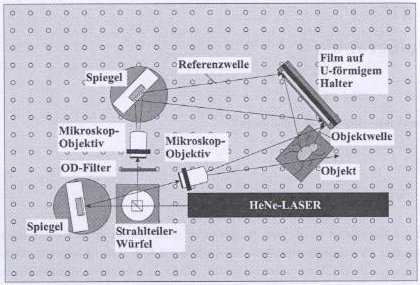
\includegraphics{grafiken/transmission}
\end{center}
\caption{Aufbau Transmissionshologramm}
\label{fig:aufbau_trans}
\end{figure}

Der Laser wird zun�chst mit dem Strahlteiler aufgeteilt und dann mit spiegeln so
geleitet, dass der aufgeweitete Referenzstrahl direkt auf den Film trifft und
der aufgeweitete Objektstrahl m�glichst gut das Objekt ausleuchtet.

Der OD-Filter dient dazu, die Intensit�ten von Referenz- und Objektstrahl
anzugleichen. Bei der Anordnung der Elemente auf dem optischen Tisch wird auf
eine m�glichst homogene Ausleuchtung des Objektes und des Filmes geachtet.
Au�erdem muss die Wegl�ngendifferenz der beiden Teilstrahlen deutlich unter der
Koh�renzl�nge des Lasers von etwa \unit[30]{cm} liegen, um an der Position des
Films Koh�renz zu gew�hrleisten, was aber kein Problem darstellte.

Nun wird der Film zun�chst belichtet (wobei die Zeiten im Skript tendenziell zu
hoch angesetzt waren) indem zun�chst der Strahl vom Laser geblockt wird und dann
f�r einige Sekunden der Strahlblocker angehoben wird um Vibrationen zu
vermeiden. In den bereitgestellten Wannen mit Entwickler, Stoppbad und
Bleichmittel wird der Film dann entwickelt und zuletzt gebleicht. Dabei war bis
zum Stoppbad der Raum nur durch eine blaue LED beleuchtet.

Nach einigen Minuten Trocknen konnten wir das dreidimensionale Abbild
beobachten, indem wir das Hologramm wieder an der selben Stelle einspannten und
den Referenzstrahl darauf richteten. Nach etwas l�ngerer Zeit war an der
Kaltlichtlampe das Bild zumindest zu erahnen (man sah die Reflexionen, aber
nicht genau das zugeh�rige Objekt), genau zu erkennen war es allerdings nicht.
Gut zu sehen war aber, dass wie erwartet nur rotes Licht gebeugt wurde.

\subsubsection{Reflexionshologramme}
F�r das Reflexionshologramm �nderten wir den Aufbau leicht ab:
\begin{figure}[h!]
\begin{center}
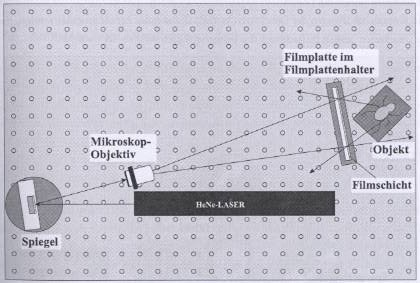
\includegraphics{grafiken/reflexion}
\end{center}
\caption{Aufbau Reflexionshologramm}
\label{fig:aufbau_ref}
\end{figure}

Es wird also im Prinzip nur das Objekt hinter dem Filmtr�ger platziert, der
Objektstrahl geblockt und der Film durch eine Photoplatte ersetzt.

Die weiter Durchf�hrung ist identisch zu der vorigen.

In diesem Versuchsteil benutzten wir wie schon erw�hnt andere Objekte, die
st�rker reflektierten. Au�erdem verwendeten wir ein kleines Auto mit Kippbild,
um zu sehen, ob dies auf dem Hologramm auch zu erkennen ist.

Unsere Reflexionshologramme wurden deutlich besser, nach entsprechend langer
Trocknungszeit waren die Hologramme auch ohne Laser sehr gut unter der
Kaltlichtlampe zu erkennen. Das Kippbild allerdings zeigte nicht das erw�nschte
Verhalten, es war aber deutlich zu sehen, dass es bei einem bestimmten Winkel
zumindest dunkel wurde, ohne aber das "`neue"' Bild zu zeigen. Vermutlich
reichte die Winkelausleuchtung einfach nicht aus, da diese Kippbilder ab einem
bestimmten Winkel mit ihren Prismen schr�g einfallendes Licht reflektieren, das
in diesem Fall ja nicht vorhanden war.

\subsubsection{Reflexionshologramm mit Quellmittel}
Im letzten Versuchsteil des ersten Versuchstages haben wir mit dem selben Aufbau
wie im vorigen Abschnitt ein weiteres Hologramm aufgenommen, diesmal aber auf
einer Photoplatte, die vor Versuchsbeginn in ein Quellmittel gelegt wurde.
Zu Erwarten ist dabei, dass wenn die photosensitive Schicht nach dem Entwickeln
und Bleichen wieder abquillt, was in Gleichungen einer nachtr�gliche
Verringerung der Gitterkonstanten bewirkt. Daher muss das Hologramm um etwas zu
sehen unter kurzwelligerem Licht betrachtet werden. Uns gelang es in der Tat
auch nicht, das Hologramm mit dem roten Laser zu rekonstruieren. Unter der
Kaltlichtlampe war aber leider auch nichts zu sehen, was uns vermuten lie�, dass
wir m�glicherweise zu lange haben Quellen lassen, weshalb sich der Bereich, in
dem das Hologramm zu sehen ist in den UV-Bereich verschob.

\subsection{Volumenhologramme in Lithiumniobat}
Am zweiten Versuchstag wird ein elementares Transmissionshologramm zuerst in
einen Lithiumniobatkristall geschrieben und dann wieder gel�scht, wobei in
beiden F�llen �ber die Zeit die Intensit�t des transmittierten und des gebeugten
Strahls gemessen wird. Im letzten Versuchsteil wird dann nach einem weiteren
Schreibvorgang die Winkelabh�ngigkeit der Beugungseffizienz untersucht. Der
Versuchsaufbau ist bei allen Teilen identisch:
\begin{figure}[h!]
\begin{center}
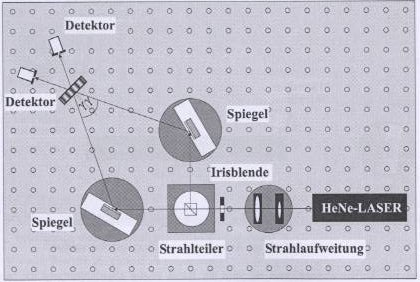
\includegraphics{grafiken/linb}
\end{center}
\caption{Aufbau Volumenholographie}
\label{fig:aufbau_vol}
\end{figure}

Um den Kristall zwischen zwei Schreibvorg�ngen m�glichst "`hologrammfrei"' zu
haben, wird er zun�chst mit einer starken Kaltlichtlampe beleuchtet, wodurch
sich �ber die Zeit eine homogene Verteilung der Ladungstr�ger ausbildet.

Beim Aufbau soll darauf geachtet werden, einen Winkel von etwa $\unit[20]{^\circ}$
zwischen den Strahlen zu und ein m�glichst gleichm��iges Ausleuchten des
Kristalls zu erhalten. Aus dem genauen Winkel von $\unit[20.1\pm 0.1]{^\circ}$ und
den bekannten Brechungsindizes von Luft und Kristall l�sst sich mit dem
Snelliusschen Brechungsgesetz der Winkel im Kristall errechnen:
\begin{align}
  \theta = \arcsin\left( \frac{n_\text{Luft}}{n_\text{Kristall}} \right)
  \sin\gamma = \unit[8.631 \pm 0.012]{^\circ}
  \label{eqn:winkel}
\end{align}

Wir messen zun�chst den Untergrund durch, f�r beide Verst�rkungen, die wir in
diesem Versuch verwendeten ($\unit[10^{-4}]{W}$ und $\unit[10^{-3}]{W}$) ergab sich
ein identischer Untergrund, den wir dann mit den reglern wegregelten. Auch die
Maxima beider Detektoren waren identisch. Wir gehen also davon aus, dass der
systematische Fehler, den wir durch direktes Verwenden der Werte bekommen
k�nnten vernachl�ssigbar sind.

\subsubsection{Schreibkurve}
Im ersten Versuchsteil nehmen wir etwa vierzig Minuten lang eine Schreibkurve
auf, wobei jede Minute der Strahl einmal unterbrochen und die Beugungseffizienz
gemessen wird. Daraus k�nnen wir wie beschrieben die Brechungsindex�nderung
$\Delta n_0$ berechnen:
\begin{align}
  \Delta n_0 = \arcsin\left( \sqrt{\eta} \right) \frac{\lambda \cos{\theta}}{\pi
  d}
\end{align}

Die Schwierigkeit hierbei bestand darin, die Apparatur wirklich v�llig still zu
halten. Die ersten $\unit[6]{min}$ im Graphen zeigen, was passiert, wenn einem
das nicht gelingt: Das eigentliche Hologramm wird langsam gel�scht und erst
danach wieder mit einem neuen �berschrieben.

Die im Graphen gezeigten Fehlerbalken sind mit einem Fehler von $\unit[\pm
0.1]{^\circ}$ und $\unit[\pm 1]{mV}$ mithilfe Gau�scher Fehlerfortpflanzung
berechnet.

\begin{figure}[H]
  \begin{tikzpicture}[gnuplot]
%% generated with GNUPLOT 4.2p6  (Lua 5.1.4; terminal rev. 90, script rev. 90)
%% Mon Mar 15 11:50:15 2010
\gpsolidlines
\gpcolor{gp lt color border}
\gpsetlinetype{gp lt border}
\gpsetlinewidth{1.00}
\draw[gp path] (2.608,0.985)--(2.788,0.985);
\draw[gp path] (12.040,0.985)--(11.860,0.985);
\node[gp node right] at (2.424,0.985) {-5e-05};
\draw[gp path] (2.608,2.218)--(2.788,2.218);
\draw[gp path] (12.040,2.218)--(11.860,2.218);
\node[gp node right] at (2.424,2.218) { 0};
\draw[gp path] (2.608,3.451)--(2.788,3.451);
\draw[gp path] (12.040,3.451)--(11.860,3.451);
\node[gp node right] at (2.424,3.451) { 5e-05};
\draw[gp path] (2.608,4.683)--(2.788,4.683);
\draw[gp path] (12.040,4.683)--(11.860,4.683);
\node[gp node right] at (2.424,4.683) { 0.0001};
\draw[gp path] (2.608,5.916)--(2.788,5.916);
\draw[gp path] (12.040,5.916)--(11.860,5.916);
\node[gp node right] at (2.424,5.916) { 0.00015};
\draw[gp path] (2.608,7.149)--(2.788,7.149);
\draw[gp path] (12.040,7.149)--(11.860,7.149);
\node[gp node right] at (2.424,7.149) { 0.0002};
\draw[gp path] (2.608,8.382)--(2.788,8.382);
\draw[gp path] (12.040,8.382)--(11.860,8.382);
\node[gp node right] at (2.424,8.382) { 0.00025};
\draw[gp path] (2.608,0.985)--(2.608,1.165);
\draw[gp path] (2.608,8.382)--(2.608,8.202);
\node[gp node center] at (2.608,0.677) {-10};
\draw[gp path] (3.955,0.985)--(3.955,1.165);
\draw[gp path] (3.955,8.382)--(3.955,8.202);
\node[gp node center] at (3.955,0.677) { 0};
\draw[gp path] (5.303,0.985)--(5.303,1.165);
\draw[gp path] (5.303,8.382)--(5.303,8.202);
\node[gp node center] at (5.303,0.677) { 10};
\draw[gp path] (6.650,0.985)--(6.650,1.165);
\draw[gp path] (6.650,8.382)--(6.650,8.202);
\node[gp node center] at (6.650,0.677) { 20};
\draw[gp path] (7.998,0.985)--(7.998,1.165);
\draw[gp path] (7.998,8.382)--(7.998,8.202);
\node[gp node center] at (7.998,0.677) { 30};
\draw[gp path] (9.345,0.985)--(9.345,1.165);
\draw[gp path] (9.345,8.382)--(9.345,8.202);
\node[gp node center] at (9.345,0.677) { 40};
\draw[gp path] (10.693,0.985)--(10.693,1.165);
\draw[gp path] (10.693,8.382)--(10.693,8.202);
\node[gp node center] at (10.693,0.677) { 50};
\draw[gp path] (12.040,0.985)--(12.040,1.165);
\draw[gp path] (12.040,8.382)--(12.040,8.202);
\node[gp node center] at (12.040,0.677) { 60};
\draw[gp path] (2.608,8.382)--(2.608,0.985)--(12.040,0.985)--(12.040,8.382)--cycle;
\node[gp node center,rotate=90] at (0.614,4.683) {$\Delta n$};
\node[gp node center] at (7.324,0.215) {$t/\unit{min}$};
\gpcolor{gp lt color 0}
\gpsetlinetype{gp lt plot 0}
\draw[gp path] (3.955,2.202)--(3.955,2.233);
\draw[gp path] (3.865,2.202)--(4.045,2.202);
\draw[gp path] (3.865,2.233)--(4.045,2.233);
\draw[gp path] (4.090,2.897)--(4.090,2.929);
\draw[gp path] (4.000,2.897)--(4.180,2.897);
\draw[gp path] (4.000,2.929)--(4.180,2.929);
\draw[gp path] (4.225,3.117)--(4.225,3.149);
\draw[gp path] (4.135,3.117)--(4.315,3.117);
\draw[gp path] (4.135,3.149)--(4.315,3.149);
\draw[gp path] (4.360,3.049)--(4.360,3.080);
\draw[gp path] (4.270,3.049)--(4.450,3.049);
\draw[gp path] (4.270,3.080)--(4.450,3.080);
\draw[gp path] (4.494,2.902)--(4.494,2.935);
\draw[gp path] (4.404,2.902)--(4.584,2.902);
\draw[gp path] (4.404,2.935)--(4.584,2.935);
\draw[gp path] (4.629,2.897)--(4.629,2.929);
\draw[gp path] (4.539,2.897)--(4.719,2.897);
\draw[gp path] (4.539,2.929)--(4.719,2.929);
\draw[gp path] (4.764,3.117)--(4.764,3.149);
\draw[gp path] (4.674,3.117)--(4.854,3.117);
\draw[gp path] (4.674,3.149)--(4.854,3.149);
\draw[gp path] (4.899,3.347)--(4.899,3.380);
\draw[gp path] (4.809,3.347)--(4.989,3.347);
\draw[gp path] (4.809,3.380)--(4.989,3.380);
\draw[gp path] (5.033,3.569)--(5.033,3.601);
\draw[gp path] (4.943,3.569)--(5.123,3.569);
\draw[gp path] (4.943,3.601)--(5.123,3.601);
\draw[gp path] (5.168,3.756)--(5.168,3.788);
\draw[gp path] (5.078,3.756)--(5.258,3.756);
\draw[gp path] (5.078,3.788)--(5.258,3.788);
\draw[gp path] (5.303,4.018)--(5.303,4.051);
\draw[gp path] (5.213,4.018)--(5.393,4.018);
\draw[gp path] (5.213,4.051)--(5.393,4.051);
\draw[gp path] (5.438,4.212)--(5.438,4.242);
\draw[gp path] (5.348,4.212)--(5.528,4.212);
\draw[gp path] (5.348,4.242)--(5.528,4.242);
\draw[gp path] (5.572,4.398)--(5.572,4.428);
\draw[gp path] (5.482,4.398)--(5.662,4.398);
\draw[gp path] (5.482,4.428)--(5.662,4.428);
\draw[gp path] (5.707,4.592)--(5.707,4.620);
\draw[gp path] (5.617,4.592)--(5.797,4.592);
\draw[gp path] (5.617,4.620)--(5.797,4.620);
\draw[gp path] (5.842,4.765)--(5.842,4.793);
\draw[gp path] (5.752,4.765)--(5.932,4.765);
\draw[gp path] (5.752,4.793)--(5.932,4.793);
\draw[gp path] (5.977,4.872)--(5.977,4.898);
\draw[gp path] (5.887,4.872)--(6.067,4.872);
\draw[gp path] (5.887,4.898)--(6.067,4.898);
\draw[gp path] (6.111,5.035)--(6.111,5.060);
\draw[gp path] (6.021,5.035)--(6.201,5.035);
\draw[gp path] (6.021,5.060)--(6.201,5.060);
\draw[gp path] (6.246,5.168)--(6.246,5.191);
\draw[gp path] (6.156,5.168)--(6.336,5.168);
\draw[gp path] (6.156,5.191)--(6.336,5.191);
\draw[gp path] (6.381,5.301)--(6.381,5.322);
\draw[gp path] (6.291,5.301)--(6.471,5.301);
\draw[gp path] (6.291,5.322)--(6.471,5.322);
\draw[gp path] (6.516,5.438)--(6.516,5.456);
\draw[gp path] (6.426,5.438)--(6.606,5.438);
\draw[gp path] (6.426,5.456)--(6.606,5.456);
\draw[gp path] (6.650,5.544)--(6.650,5.561);
\draw[gp path] (6.560,5.544)--(6.740,5.544);
\draw[gp path] (6.560,5.561)--(6.740,5.561);
\draw[gp path] (6.785,5.688)--(6.785,5.703);
\draw[gp path] (6.695,5.688)--(6.875,5.688);
\draw[gp path] (6.695,5.703)--(6.875,5.703);
\draw[gp path] (6.920,5.832)--(6.920,5.844);
\draw[gp path] (6.830,5.832)--(7.010,5.832);
\draw[gp path] (6.830,5.844)--(7.010,5.844);
\draw[gp path] (7.055,5.943)--(7.055,5.953);
\draw[gp path] (6.965,5.943)--(7.145,5.943);
\draw[gp path] (6.965,5.953)--(7.145,5.953);
\draw[gp path] (7.189,6.065)--(7.189,6.074);
\draw[gp path] (7.099,6.065)--(7.279,6.065);
\draw[gp path] (7.099,6.074)--(7.279,6.074);
\draw[gp path] (7.324,6.212)--(7.324,6.219);
\draw[gp path] (7.234,6.212)--(7.414,6.212);
\draw[gp path] (7.234,6.219)--(7.414,6.219);
\draw[gp path] (7.459,6.334)--(7.459,6.339);
\draw[gp path] (7.369,6.334)--(7.549,6.334);
\draw[gp path] (7.369,6.339)--(7.549,6.339);
\draw[gp path] (7.593,6.446)--(7.593,6.450);
\draw[gp path] (7.503,6.446)--(7.683,6.446);
\draw[gp path] (7.503,6.450)--(7.683,6.450);
\draw[gp path] (7.728,6.560)--(7.728,6.564);
\draw[gp path] (7.638,6.560)--(7.818,6.560);
\draw[gp path] (7.638,6.564)--(7.818,6.564);
\draw[gp path] (7.863,6.654)--(7.863,6.656);
\draw[gp path] (7.773,6.654)--(7.953,6.654);
\draw[gp path] (7.773,6.656)--(7.953,6.656);
\draw[gp path] (7.998,6.767)--(7.998,6.769);
\draw[gp path] (7.908,6.767)--(8.088,6.767);
\draw[gp path] (7.908,6.769)--(8.088,6.769);
\draw[gp path] (8.132,6.857)--(8.132,6.859);
\draw[gp path] (8.042,6.857)--(8.222,6.857);
\draw[gp path] (8.042,6.859)--(8.222,6.859);
\draw[gp path] (8.267,6.943)--(8.267,6.944);
\draw[gp path] (8.177,6.943)--(8.357,6.943);
\draw[gp path] (8.177,6.944)--(8.357,6.944);
\draw[gp path] (8.402,7.024)--(8.402,7.025);
\draw[gp path] (8.312,7.024)--(8.492,7.024);
\draw[gp path] (8.312,7.025)--(8.492,7.025);
\draw[gp path] (8.537,7.114)--(8.537,7.115);
\draw[gp path] (8.447,7.114)--(8.627,7.114);
\draw[gp path] (8.447,7.115)--(8.627,7.115);
\draw[gp path] (8.581,7.190)--(8.761,7.190);
\draw[gp path] (8.581,7.190)--(8.761,7.190);
\draw[gp path] (8.716,7.270)--(8.896,7.270);
\draw[gp path] (8.716,7.270)--(8.896,7.270);
\draw[gp path] (8.851,7.358)--(9.031,7.358);
\draw[gp path] (8.851,7.358)--(9.031,7.358);
\draw[gp path] (9.076,7.433)--(9.076,7.434);
\draw[gp path] (8.986,7.433)--(9.166,7.433);
\draw[gp path] (8.986,7.434)--(9.166,7.434);
\draw[gp path] (9.120,7.504)--(9.300,7.504);
\draw[gp path] (9.120,7.504)--(9.300,7.504);
\draw[gp path] (9.255,7.566)--(9.435,7.566);
\draw[gp path] (9.255,7.566)--(9.435,7.566);
\draw[gp path] (9.480,7.635)--(9.480,7.636);
\draw[gp path] (9.390,7.635)--(9.570,7.635);
\draw[gp path] (9.390,7.636)--(9.570,7.636);
\draw[gp path] (9.525,7.698)--(9.705,7.698);
\draw[gp path] (9.525,7.698)--(9.705,7.698);
\draw[gp path] (9.659,7.753)--(9.839,7.753);
\draw[gp path] (9.659,7.753)--(9.839,7.753);
\draw[gp path] (9.794,7.821)--(9.974,7.821);
\draw[gp path] (9.794,7.821)--(9.974,7.821);
\draw[gp path] (9.929,7.876)--(10.109,7.876);
\draw[gp path] (9.929,7.876)--(10.109,7.876);
\draw[gp path] (10.064,7.920)--(10.244,7.920);
\draw[gp path] (10.064,7.920)--(10.244,7.920);
\draw[gp path] (10.198,7.989)--(10.378,7.989);
\draw[gp path] (10.198,7.989)--(10.378,7.989);
\draw[gp path] (10.333,8.029)--(10.513,8.029);
\draw[gp path] (10.333,8.029)--(10.513,8.029);
\draw[gp path] (10.468,8.082)--(10.648,8.082);
\draw[gp path] (10.468,8.082)--(10.648,8.082);
\draw[gp path] (10.603,8.126)--(10.783,8.126);
\draw[gp path] (10.603,8.126)--(10.783,8.126);
\draw[gp path] (10.737,8.156)--(10.917,8.156);
\draw[gp path] (10.737,8.156)--(10.917,8.156);
\draw[gp path] (10.872,8.201)--(11.052,8.201);
\draw[gp path] (10.872,8.201)--(11.052,8.201);
\draw[gp path] (11.007,8.230)--(11.187,8.230);
\draw[gp path] (11.007,8.230)--(11.187,8.230);
\draw[gp path] (3.942,2.218)--(3.969,2.218);
\draw[gp path] (3.942,2.128)--(3.942,2.308);
\draw[gp path] (3.969,2.128)--(3.969,2.308);
\draw[gp path] (4.077,2.913)--(4.104,2.913);
\draw[gp path] (4.077,2.823)--(4.077,3.003);
\draw[gp path] (4.104,2.823)--(4.104,3.003);
\draw[gp path] (4.211,3.133)--(4.238,3.133);
\draw[gp path] (4.211,3.043)--(4.211,3.223);
\draw[gp path] (4.238,3.043)--(4.238,3.223);
\draw[gp path] (4.346,3.064)--(4.373,3.064);
\draw[gp path] (4.346,2.974)--(4.346,3.154);
\draw[gp path] (4.373,2.974)--(4.373,3.154);
\draw[gp path] (4.481,2.918)--(4.508,2.918);
\draw[gp path] (4.481,2.828)--(4.481,3.008);
\draw[gp path] (4.508,2.828)--(4.508,3.008);
\draw[gp path] (4.616,2.913)--(4.643,2.913);
\draw[gp path] (4.616,2.823)--(4.616,3.003);
\draw[gp path] (4.643,2.823)--(4.643,3.003);
\draw[gp path] (4.750,3.133)--(4.777,3.133);
\draw[gp path] (4.750,3.043)--(4.750,3.223);
\draw[gp path] (4.777,3.043)--(4.777,3.223);
\draw[gp path] (4.885,3.363)--(4.912,3.363);
\draw[gp path] (4.885,3.273)--(4.885,3.453);
\draw[gp path] (4.912,3.273)--(4.912,3.453);
\draw[gp path] (5.020,3.585)--(5.047,3.585);
\draw[gp path] (5.020,3.495)--(5.020,3.675);
\draw[gp path] (5.047,3.495)--(5.047,3.675);
\draw[gp path] (5.155,3.772)--(5.182,3.772);
\draw[gp path] (5.155,3.682)--(5.155,3.862);
\draw[gp path] (5.182,3.682)--(5.182,3.862);
\draw[gp path] (5.289,4.034)--(5.316,4.034);
\draw[gp path] (5.289,3.944)--(5.289,4.124);
\draw[gp path] (5.316,3.944)--(5.316,4.124);
\draw[gp path] (5.424,4.227)--(5.451,4.227);
\draw[gp path] (5.424,4.137)--(5.424,4.317);
\draw[gp path] (5.451,4.137)--(5.451,4.317);
\draw[gp path] (5.559,4.413)--(5.586,4.413);
\draw[gp path] (5.559,4.323)--(5.559,4.503);
\draw[gp path] (5.586,4.323)--(5.586,4.503);
\draw[gp path] (5.694,4.606)--(5.721,4.606);
\draw[gp path] (5.694,4.516)--(5.694,4.696);
\draw[gp path] (5.721,4.516)--(5.721,4.696);
\draw[gp path] (5.828,4.779)--(5.855,4.779);
\draw[gp path] (5.828,4.689)--(5.828,4.869);
\draw[gp path] (5.855,4.689)--(5.855,4.869);
\draw[gp path] (5.963,4.885)--(5.990,4.885);
\draw[gp path] (5.963,4.795)--(5.963,4.975);
\draw[gp path] (5.990,4.795)--(5.990,4.975);
\draw[gp path] (6.098,5.047)--(6.125,5.047);
\draw[gp path] (6.098,4.957)--(6.098,5.137);
\draw[gp path] (6.125,4.957)--(6.125,5.137);
\draw[gp path] (6.233,5.180)--(6.260,5.180);
\draw[gp path] (6.233,5.090)--(6.233,5.270);
\draw[gp path] (6.260,5.090)--(6.260,5.270);
\draw[gp path] (6.367,5.312)--(6.394,5.312);
\draw[gp path] (6.367,5.222)--(6.367,5.402);
\draw[gp path] (6.394,5.222)--(6.394,5.402);
\draw[gp path] (6.502,5.447)--(6.529,5.447);
\draw[gp path] (6.502,5.357)--(6.502,5.537);
\draw[gp path] (6.529,5.357)--(6.529,5.537);
\draw[gp path] (6.637,5.553)--(6.664,5.553);
\draw[gp path] (6.637,5.463)--(6.637,5.643);
\draw[gp path] (6.664,5.463)--(6.664,5.643);
\draw[gp path] (6.772,5.696)--(6.799,5.696);
\draw[gp path] (6.772,5.606)--(6.772,5.786);
\draw[gp path] (6.799,5.606)--(6.799,5.786);
\draw[gp path] (6.906,5.838)--(6.933,5.838);
\draw[gp path] (6.906,5.748)--(6.906,5.928);
\draw[gp path] (6.933,5.748)--(6.933,5.928);
\draw[gp path] (7.041,5.948)--(7.068,5.948);
\draw[gp path] (7.041,5.858)--(7.041,6.038);
\draw[gp path] (7.068,5.858)--(7.068,6.038);
\draw[gp path] (7.176,6.069)--(7.203,6.069);
\draw[gp path] (7.176,5.979)--(7.176,6.159);
\draw[gp path] (7.203,5.979)--(7.203,6.159);
\draw[gp path] (7.311,6.215)--(7.337,6.215);
\draw[gp path] (7.311,6.125)--(7.311,6.305);
\draw[gp path] (7.337,6.125)--(7.337,6.305);
\draw[gp path] (7.445,6.337)--(7.472,6.337);
\draw[gp path] (7.445,6.247)--(7.445,6.427);
\draw[gp path] (7.472,6.247)--(7.472,6.427);
\draw[gp path] (7.580,6.448)--(7.607,6.448);
\draw[gp path] (7.580,6.358)--(7.580,6.538);
\draw[gp path] (7.607,6.358)--(7.607,6.538);
\draw[gp path] (7.715,6.562)--(7.742,6.562);
\draw[gp path] (7.715,6.472)--(7.715,6.652);
\draw[gp path] (7.742,6.472)--(7.742,6.652);
\draw[gp path] (7.849,6.655)--(7.876,6.655);
\draw[gp path] (7.849,6.565)--(7.849,6.745);
\draw[gp path] (7.876,6.565)--(7.876,6.745);
\draw[gp path] (7.984,6.768)--(8.011,6.768);
\draw[gp path] (7.984,6.678)--(7.984,6.858);
\draw[gp path] (8.011,6.678)--(8.011,6.858);
\draw[gp path] (8.119,6.858)--(8.146,6.858);
\draw[gp path] (8.119,6.768)--(8.119,6.948);
\draw[gp path] (8.146,6.768)--(8.146,6.948);
\draw[gp path] (8.254,6.943)--(8.281,6.943);
\draw[gp path] (8.254,6.853)--(8.254,7.033);
\draw[gp path] (8.281,6.853)--(8.281,7.033);
\draw[gp path] (8.388,7.025)--(8.415,7.025);
\draw[gp path] (8.388,6.935)--(8.388,7.115);
\draw[gp path] (8.415,6.935)--(8.415,7.115);
\draw[gp path] (8.523,7.115)--(8.550,7.115);
\draw[gp path] (8.523,7.025)--(8.523,7.205);
\draw[gp path] (8.550,7.025)--(8.550,7.205);
\draw[gp path] (8.658,7.190)--(8.685,7.190);
\draw[gp path] (8.658,7.100)--(8.658,7.280);
\draw[gp path] (8.685,7.100)--(8.685,7.280);
\draw[gp path] (8.793,7.270)--(8.820,7.270);
\draw[gp path] (8.793,7.180)--(8.793,7.360);
\draw[gp path] (8.820,7.180)--(8.820,7.360);
\draw[gp path] (8.927,7.358)--(8.954,7.358);
\draw[gp path] (8.927,7.268)--(8.927,7.448);
\draw[gp path] (8.954,7.268)--(8.954,7.448);
\draw[gp path] (9.062,7.433)--(9.089,7.433);
\draw[gp path] (9.062,7.343)--(9.062,7.523);
\draw[gp path] (9.089,7.343)--(9.089,7.523);
\draw[gp path] (9.197,7.504)--(9.224,7.504);
\draw[gp path] (9.197,7.414)--(9.197,7.594);
\draw[gp path] (9.224,7.414)--(9.224,7.594);
\draw[gp path] (9.332,7.566)--(9.359,7.566);
\draw[gp path] (9.332,7.476)--(9.332,7.656);
\draw[gp path] (9.359,7.476)--(9.359,7.656);
\draw[gp path] (9.466,7.635)--(9.493,7.635);
\draw[gp path] (9.466,7.545)--(9.466,7.725);
\draw[gp path] (9.493,7.545)--(9.493,7.725);
\draw[gp path] (9.601,7.698)--(9.628,7.698);
\draw[gp path] (9.601,7.608)--(9.601,7.788);
\draw[gp path] (9.628,7.608)--(9.628,7.788);
\draw[gp path] (9.736,7.753)--(9.763,7.753);
\draw[gp path] (9.736,7.663)--(9.736,7.843);
\draw[gp path] (9.763,7.663)--(9.763,7.843);
\draw[gp path] (9.871,7.821)--(9.898,7.821);
\draw[gp path] (9.871,7.731)--(9.871,7.911);
\draw[gp path] (9.898,7.731)--(9.898,7.911);
\draw[gp path] (10.005,7.876)--(10.032,7.876);
\draw[gp path] (10.005,7.786)--(10.005,7.966);
\draw[gp path] (10.032,7.786)--(10.032,7.966);
\draw[gp path] (10.140,7.920)--(10.167,7.920);
\draw[gp path] (10.140,7.830)--(10.140,8.010);
\draw[gp path] (10.167,7.830)--(10.167,8.010);
\draw[gp path] (10.275,7.989)--(10.302,7.989);
\draw[gp path] (10.275,7.899)--(10.275,8.079);
\draw[gp path] (10.302,7.899)--(10.302,8.079);
\draw[gp path] (10.410,8.029)--(10.437,8.029);
\draw[gp path] (10.410,7.939)--(10.410,8.119);
\draw[gp path] (10.437,7.939)--(10.437,8.119);
\draw[gp path] (10.544,8.082)--(10.571,8.082);
\draw[gp path] (10.544,7.992)--(10.544,8.172);
\draw[gp path] (10.571,7.992)--(10.571,8.172);
\draw[gp path] (10.679,8.126)--(10.706,8.126);
\draw[gp path] (10.679,8.036)--(10.679,8.216);
\draw[gp path] (10.706,8.036)--(10.706,8.216);
\draw[gp path] (10.814,8.156)--(10.841,8.156);
\draw[gp path] (10.814,8.066)--(10.814,8.246);
\draw[gp path] (10.841,8.066)--(10.841,8.246);
\draw[gp path] (10.949,8.201)--(10.976,8.201);
\draw[gp path] (10.949,8.111)--(10.949,8.291);
\draw[gp path] (10.976,8.111)--(10.976,8.291);
\draw[gp path] (11.083,8.230)--(11.110,8.230);
\draw[gp path] (11.083,8.140)--(11.083,8.320);
\draw[gp path] (11.110,8.140)--(11.110,8.320);
\gpsetpointsize{4.00}
\gppoint{gp mark 1}{(3.955,2.218)}
\gppoint{gp mark 1}{(4.090,2.913)}
\gppoint{gp mark 1}{(4.225,3.133)}
\gppoint{gp mark 1}{(4.360,3.064)}
\gppoint{gp mark 1}{(4.494,2.918)}
\gppoint{gp mark 1}{(4.629,2.913)}
\gppoint{gp mark 1}{(4.764,3.133)}
\gppoint{gp mark 1}{(4.899,3.363)}
\gppoint{gp mark 1}{(5.033,3.585)}
\gppoint{gp mark 1}{(5.168,3.772)}
\gppoint{gp mark 1}{(5.303,4.034)}
\gppoint{gp mark 1}{(5.438,4.227)}
\gppoint{gp mark 1}{(5.572,4.413)}
\gppoint{gp mark 1}{(5.707,4.606)}
\gppoint{gp mark 1}{(5.842,4.779)}
\gppoint{gp mark 1}{(5.977,4.885)}
\gppoint{gp mark 1}{(6.111,5.047)}
\gppoint{gp mark 1}{(6.246,5.180)}
\gppoint{gp mark 1}{(6.381,5.312)}
\gppoint{gp mark 1}{(6.516,5.447)}
\gppoint{gp mark 1}{(6.650,5.553)}
\gppoint{gp mark 1}{(6.785,5.696)}
\gppoint{gp mark 1}{(6.920,5.838)}
\gppoint{gp mark 1}{(7.055,5.948)}
\gppoint{gp mark 1}{(7.189,6.069)}
\gppoint{gp mark 1}{(7.324,6.215)}
\gppoint{gp mark 1}{(7.459,6.337)}
\gppoint{gp mark 1}{(7.593,6.448)}
\gppoint{gp mark 1}{(7.728,6.562)}
\gppoint{gp mark 1}{(7.863,6.655)}
\gppoint{gp mark 1}{(7.998,6.768)}
\gppoint{gp mark 1}{(8.132,6.858)}
\gppoint{gp mark 1}{(8.267,6.943)}
\gppoint{gp mark 1}{(8.402,7.025)}
\gppoint{gp mark 1}{(8.537,7.115)}
\gppoint{gp mark 1}{(8.671,7.190)}
\gppoint{gp mark 1}{(8.806,7.270)}
\gppoint{gp mark 1}{(8.941,7.358)}
\gppoint{gp mark 1}{(9.076,7.433)}
\gppoint{gp mark 1}{(9.210,7.504)}
\gppoint{gp mark 1}{(9.345,7.566)}
\gppoint{gp mark 1}{(9.480,7.635)}
\gppoint{gp mark 1}{(9.615,7.698)}
\gppoint{gp mark 1}{(9.749,7.753)}
\gppoint{gp mark 1}{(9.884,7.821)}
\gppoint{gp mark 1}{(10.019,7.876)}
\gppoint{gp mark 1}{(10.154,7.920)}
\gppoint{gp mark 1}{(10.288,7.989)}
\gppoint{gp mark 1}{(10.423,8.029)}
\gppoint{gp mark 1}{(10.558,8.082)}
\gppoint{gp mark 1}{(10.693,8.126)}
\gppoint{gp mark 1}{(10.827,8.156)}
\gppoint{gp mark 1}{(10.962,8.201)}
\gppoint{gp mark 1}{(11.097,8.230)}
\gpcolor{gp lt color 1}
\gpsetlinetype{gp lt plot 1}
\draw[gp path] (3.942,1.683)--(4.014,1.827)--(4.087,1.969)--(4.159,2.108)--(4.232,2.245)%
  --(4.304,2.379)--(4.376,2.511)--(4.449,2.640)--(4.521,2.767)--(4.594,2.891)--(4.666,3.014)%
  --(4.738,3.133)--(4.811,3.251)--(4.883,3.367)--(4.956,3.480)--(5.028,3.591)--(5.100,3.701)%
  --(5.173,3.808)--(5.245,3.913)--(5.318,4.016)--(5.390,4.118)--(5.463,4.217)--(5.535,4.315)%
  --(5.607,4.411)--(5.680,4.505)--(5.752,4.597)--(5.825,4.688)--(5.897,4.777)--(5.969,4.864)%
  --(6.042,4.950)--(6.114,5.034)--(6.187,5.117)--(6.259,5.198)--(6.331,5.277)--(6.404,5.355)%
  --(6.476,5.432)--(6.549,5.507)--(6.621,5.581)--(6.693,5.653)--(6.766,5.724)--(6.838,5.794)%
  --(6.911,5.863)--(6.983,5.930)--(7.055,5.996)--(7.128,6.061)--(7.200,6.124)--(7.273,6.187)%
  --(7.345,6.248)--(7.418,6.308)--(7.490,6.367)--(7.562,6.425)--(7.635,6.482)--(7.707,6.537)%
  --(7.780,6.592)--(7.852,6.646)--(7.924,6.699)--(7.997,6.750)--(8.069,6.801)--(8.142,6.851)%
  --(8.214,6.900)--(8.286,6.948)--(8.359,6.995)--(8.431,7.041)--(8.504,7.087)--(8.576,7.131)%
  --(8.648,7.175)--(8.721,7.218)--(8.793,7.260)--(8.866,7.302)--(8.938,7.342)--(9.010,7.382)%
  --(9.083,7.421)--(9.155,7.460)--(9.228,7.497)--(9.300,7.534)--(9.372,7.571)--(9.445,7.606)%
  --(9.517,7.641)--(9.590,7.675)--(9.662,7.709)--(9.735,7.742)--(9.807,7.775)--(9.879,7.806)%
  --(9.952,7.838)--(10.024,7.868)--(10.097,7.899)--(10.169,7.928)--(10.241,7.957)--(10.314,7.986)%
  --(10.386,8.014)--(10.459,8.041)--(10.531,8.068)--(10.603,8.094)--(10.676,8.120)--(10.748,8.146)%
  --(10.821,8.171)--(10.893,8.195)--(10.965,8.219)--(11.038,8.243)--(11.110,8.266);
\gpcolor{gp lt color border}
\gpsetlinetype{gp lt border}
\draw[gp path] (2.608,8.382)--(2.608,0.985)--(12.040,0.985)--(12.040,8.382)--cycle;
%% coordinates of the plot area
\gpdefrectangularnode{gp plot 1}{\pgfpoint{2.608cm}{0.985cm}}{\pgfpoint{12.040cm}{8.382cm}}
\end{tikzpicture}
%% gnuplot variables

  \caption{Schreibkurve und exponentieller Fit}
  \label{fig:schreibkurve}
\end{figure}

Wie im Theorieteil beschrieben fitten wir daran die Funktion $\Delta n(t) =
\Delta n_\text{max}\left( 1 - \exp\left( -\frac{t}{\tau} \right) \right)$.

In Abbildung \ref{fig:schreibkurve} ist die Schreibkurve mit dem Fit zu sehen.
Wir erhalten aus dem Fit die Werte:
\begin{align}
  \Delta n_\text{max} &= \unit[(18.09 \pm 0.06)]{10^{-3}} \\
  \tau &= \unit[(26.78 \pm 39)]{min}
  \label{eqn:werte_schreibkurve}
\end{align}

\subsubsection{L�schkurve}
Die L�schkurve wird aufgenommen, indem �ber eine lange Zeit nur der Lesestrahl
auf das Hologramm gerichtet ist. Durch diese homogene Beleuchtung wird
gleichzeitig das geschriebene Hologramm wieder gel�scht. Da die Wellenamplitude 
nur noch halb so gro� ist wie beim Schreiben und damit die Intensit�t nur noch
ein Viertel betr�gt erwarten wir, dass $\tau$ in diesem Fall $4$ mal so gro� ist
wie beim schreiben. Die L�schkurve sieht wie folgt aus:

\begin{figure}[H]
  \begin{tikzpicture}[gnuplot]
%% generated with GNUPLOT 4.2p6  (Lua 5.1.4; terminal rev. 90, script rev. 90)
%% Mon Mar 15 11:50:15 2010
\gpsolidlines
\gpcolor{gp lt color border}
\gpsetlinetype{gp lt border}
\gpsetlinewidth{1.00}
\draw[gp path] (2.792,0.985)--(2.972,0.985);
\draw[gp path] (12.040,0.985)--(11.860,0.985);
\node[gp node right] at (2.608,0.985) { 0.000224};
\draw[gp path] (2.792,1.807)--(2.972,1.807);
\draw[gp path] (12.040,1.807)--(11.860,1.807);
\node[gp node right] at (2.608,1.807) { 0.000226};
\draw[gp path] (2.792,2.629)--(2.972,2.629);
\draw[gp path] (12.040,2.629)--(11.860,2.629);
\node[gp node right] at (2.608,2.629) { 0.000228};
\draw[gp path] (2.792,3.451)--(2.972,3.451);
\draw[gp path] (12.040,3.451)--(11.860,3.451);
\node[gp node right] at (2.608,3.451) { 0.00023};
\draw[gp path] (2.792,4.273)--(2.972,4.273);
\draw[gp path] (12.040,4.273)--(11.860,4.273);
\node[gp node right] at (2.608,4.273) { 0.000232};
\draw[gp path] (2.792,5.094)--(2.972,5.094);
\draw[gp path] (12.040,5.094)--(11.860,5.094);
\node[gp node right] at (2.608,5.094) { 0.000234};
\draw[gp path] (2.792,5.916)--(2.972,5.916);
\draw[gp path] (12.040,5.916)--(11.860,5.916);
\node[gp node right] at (2.608,5.916) { 0.000236};
\draw[gp path] (2.792,6.738)--(2.972,6.738);
\draw[gp path] (12.040,6.738)--(11.860,6.738);
\node[gp node right] at (2.608,6.738) { 0.000238};
\draw[gp path] (2.792,7.560)--(2.972,7.560);
\draw[gp path] (12.040,7.560)--(11.860,7.560);
\node[gp node right] at (2.608,7.560) { 0.00024};
\draw[gp path] (2.792,8.382)--(2.972,8.382);
\draw[gp path] (12.040,8.382)--(11.860,8.382);
\node[gp node right] at (2.608,8.382) { 0.000242};
\draw[gp path] (2.792,0.985)--(2.792,1.165);
\draw[gp path] (2.792,8.382)--(2.792,8.202);
\node[gp node center] at (2.792,0.677) { 0};
\draw[gp path] (4.333,0.985)--(4.333,1.165);
\draw[gp path] (4.333,8.382)--(4.333,8.202);
\node[gp node center] at (4.333,0.677) { 10};
\draw[gp path] (5.875,0.985)--(5.875,1.165);
\draw[gp path] (5.875,8.382)--(5.875,8.202);
\node[gp node center] at (5.875,0.677) { 20};
\draw[gp path] (7.416,0.985)--(7.416,1.165);
\draw[gp path] (7.416,8.382)--(7.416,8.202);
\node[gp node center] at (7.416,0.677) { 30};
\draw[gp path] (8.957,0.985)--(8.957,1.165);
\draw[gp path] (8.957,8.382)--(8.957,8.202);
\node[gp node center] at (8.957,0.677) { 40};
\draw[gp path] (10.499,0.985)--(10.499,1.165);
\draw[gp path] (10.499,8.382)--(10.499,8.202);
\node[gp node center] at (10.499,0.677) { 50};
\draw[gp path] (12.040,0.985)--(12.040,1.165);
\draw[gp path] (12.040,8.382)--(12.040,8.202);
\node[gp node center] at (12.040,0.677) { 60};
\draw[gp path] (2.792,8.382)--(2.792,0.985)--(12.040,0.985)--(12.040,8.382)--cycle;
\node[gp node center,rotate=90] at (0.614,4.683) {$\Delta n$};
\node[gp node center] at (7.416,0.215) {$t/\unit{min}$};
\gpcolor{gp lt color 0}
\gpsetlinetype{gp lt plot 0}
\draw[gp path] (2.946,8.035)--(2.946,8.341);
\draw[gp path] (2.856,8.035)--(3.036,8.035);
\draw[gp path] (2.856,8.341)--(3.036,8.341);
\draw[gp path] (3.100,7.760)--(3.100,8.084);
\draw[gp path] (3.010,7.760)--(3.190,7.760);
\draw[gp path] (3.010,8.084)--(3.190,8.084);
\draw[gp path] (3.254,7.653)--(3.254,7.965);
\draw[gp path] (3.164,7.653)--(3.344,7.653);
\draw[gp path] (3.164,7.965)--(3.344,7.965);
\draw[gp path] (3.409,7.564)--(3.409,7.894);
\draw[gp path] (3.319,7.564)--(3.499,7.564);
\draw[gp path] (3.319,7.894)--(3.499,7.894);
\draw[gp path] (3.563,7.576)--(3.563,7.886);
\draw[gp path] (3.473,7.576)--(3.653,7.576);
\draw[gp path] (3.473,7.886)--(3.653,7.886);
\draw[gp path] (3.717,7.404)--(3.717,7.731);
\draw[gp path] (3.627,7.404)--(3.807,7.404);
\draw[gp path] (3.627,7.731)--(3.807,7.731);
\draw[gp path] (3.871,7.242)--(3.871,7.579);
\draw[gp path] (3.781,7.242)--(3.961,7.242);
\draw[gp path] (3.781,7.579)--(3.961,7.579);
\draw[gp path] (4.025,7.153)--(4.025,7.493);
\draw[gp path] (3.935,7.153)--(4.115,7.153);
\draw[gp path] (3.935,7.493)--(4.115,7.493);
\draw[gp path] (4.179,7.091)--(4.179,7.425);
\draw[gp path] (4.089,7.091)--(4.269,7.091);
\draw[gp path] (4.089,7.425)--(4.269,7.425);
\draw[gp path] (4.333,6.940)--(4.333,7.271);
\draw[gp path] (4.243,6.940)--(4.423,6.940);
\draw[gp path] (4.243,7.271)--(4.423,7.271);
\draw[gp path] (4.487,6.831)--(4.487,7.168);
\draw[gp path] (4.397,6.831)--(4.577,6.831);
\draw[gp path] (4.397,7.168)--(4.577,7.168);
\draw[gp path] (4.642,6.694)--(4.642,7.033);
\draw[gp path] (4.552,6.694)--(4.732,6.694);
\draw[gp path] (4.552,7.033)--(4.732,7.033);
\draw[gp path] (4.796,6.564)--(4.796,6.907);
\draw[gp path] (4.706,6.564)--(4.886,6.564);
\draw[gp path] (4.706,6.907)--(4.886,6.907);
\draw[gp path] (4.950,6.418)--(4.950,6.765);
\draw[gp path] (4.860,6.418)--(5.040,6.418);
\draw[gp path] (4.860,6.765)--(5.040,6.765);
\draw[gp path] (5.104,6.257)--(5.104,6.604);
\draw[gp path] (5.014,6.257)--(5.194,6.257);
\draw[gp path] (5.014,6.604)--(5.194,6.604);
\draw[gp path] (5.258,6.126)--(5.258,6.478);
\draw[gp path] (5.168,6.126)--(5.348,6.126);
\draw[gp path] (5.168,6.478)--(5.348,6.478);
\draw[gp path] (5.412,5.973)--(5.412,6.329);
\draw[gp path] (5.322,5.973)--(5.502,5.973);
\draw[gp path] (5.322,6.329)--(5.502,6.329);
\draw[gp path] (5.566,5.841)--(5.566,6.202);
\draw[gp path] (5.476,5.841)--(5.656,5.841);
\draw[gp path] (5.476,6.202)--(5.656,6.202);
\draw[gp path] (5.721,5.669)--(5.721,6.038);
\draw[gp path] (5.631,5.669)--(5.811,5.669);
\draw[gp path] (5.631,6.038)--(5.811,6.038);
\draw[gp path] (5.875,5.551)--(5.875,5.916);
\draw[gp path] (5.785,5.551)--(5.965,5.551);
\draw[gp path] (5.785,5.916)--(5.965,5.916);
\draw[gp path] (6.029,5.409)--(6.029,5.777);
\draw[gp path] (5.939,5.409)--(6.119,5.409);
\draw[gp path] (5.939,5.777)--(6.119,5.777);
\draw[gp path] (6.183,5.044)--(6.183,5.433);
\draw[gp path] (6.093,5.044)--(6.273,5.044);
\draw[gp path] (6.093,5.433)--(6.273,5.433);
\draw[gp path] (6.337,5.005)--(6.337,5.397);
\draw[gp path] (6.247,5.005)--(6.427,5.005);
\draw[gp path] (6.247,5.397)--(6.427,5.397);
\draw[gp path] (6.491,4.930)--(6.491,5.333);
\draw[gp path] (6.401,4.930)--(6.581,4.930);
\draw[gp path] (6.401,5.333)--(6.581,5.333);
\draw[gp path] (6.645,4.860)--(6.645,5.268);
\draw[gp path] (6.555,4.860)--(6.735,4.860);
\draw[gp path] (6.555,5.268)--(6.735,5.268);
\draw[gp path] (6.799,4.792)--(6.799,5.198);
\draw[gp path] (6.709,4.792)--(6.889,4.792);
\draw[gp path] (6.709,5.198)--(6.889,5.198);
\draw[gp path] (6.954,4.684)--(6.954,5.095);
\draw[gp path] (6.864,4.684)--(7.044,4.684);
\draw[gp path] (6.864,5.095)--(7.044,5.095);
\draw[gp path] (7.108,4.537)--(7.108,4.953);
\draw[gp path] (7.018,4.537)--(7.198,4.537);
\draw[gp path] (7.018,4.953)--(7.198,4.953);
\draw[gp path] (7.262,4.438)--(7.262,4.855);
\draw[gp path] (7.172,4.438)--(7.352,4.438);
\draw[gp path] (7.172,4.855)--(7.352,4.855);
\draw[gp path] (7.416,4.328)--(7.416,4.739);
\draw[gp path] (7.326,4.328)--(7.506,4.328);
\draw[gp path] (7.326,4.739)--(7.506,4.739);
\draw[gp path] (7.570,4.139)--(7.570,4.542);
\draw[gp path] (7.480,4.139)--(7.660,4.139);
\draw[gp path] (7.480,4.542)--(7.660,4.542);
\draw[gp path] (7.724,4.065)--(7.724,4.475);
\draw[gp path] (7.634,4.065)--(7.814,4.065);
\draw[gp path] (7.634,4.475)--(7.814,4.475);
\draw[gp path] (7.878,3.879)--(7.878,4.288);
\draw[gp path] (7.788,3.879)--(7.968,3.879);
\draw[gp path] (7.788,4.288)--(7.968,4.288);
\draw[gp path] (8.033,3.691)--(8.033,4.106);
\draw[gp path] (7.943,3.691)--(8.123,3.691);
\draw[gp path] (7.943,4.106)--(8.123,4.106);
\draw[gp path] (8.187,3.612)--(8.187,4.029);
\draw[gp path] (8.097,3.612)--(8.277,3.612);
\draw[gp path] (8.097,4.029)--(8.277,4.029);
\draw[gp path] (8.341,3.468)--(8.341,3.887);
\draw[gp path] (8.251,3.468)--(8.431,3.468);
\draw[gp path] (8.251,3.887)--(8.431,3.887);
\draw[gp path] (8.495,3.264)--(8.495,3.693);
\draw[gp path] (8.405,3.264)--(8.585,3.264);
\draw[gp path] (8.405,3.693)--(8.585,3.693);
\draw[gp path] (8.649,3.157)--(8.649,3.587);
\draw[gp path] (8.559,3.157)--(8.739,3.157);
\draw[gp path] (8.559,3.587)--(8.739,3.587);
\draw[gp path] (8.803,3.015)--(8.803,3.450);
\draw[gp path] (8.713,3.015)--(8.893,3.015);
\draw[gp path] (8.713,3.450)--(8.893,3.450);
\draw[gp path] (8.957,2.896)--(8.957,3.335);
\draw[gp path] (8.867,2.896)--(9.047,2.896);
\draw[gp path] (8.867,3.335)--(9.047,3.335);
\draw[gp path] (9.111,2.740)--(9.111,3.186);
\draw[gp path] (9.021,2.740)--(9.201,2.740);
\draw[gp path] (9.021,3.186)--(9.201,3.186);
\draw[gp path] (9.266,2.626)--(9.266,3.077);
\draw[gp path] (9.176,2.626)--(9.356,2.626);
\draw[gp path] (9.176,3.077)--(9.356,3.077);
\draw[gp path] (9.420,2.446)--(9.420,2.906);
\draw[gp path] (9.330,2.446)--(9.510,2.446);
\draw[gp path] (9.330,2.906)--(9.510,2.906);
\draw[gp path] (9.574,2.317)--(9.574,2.784);
\draw[gp path] (9.484,2.317)--(9.664,2.317);
\draw[gp path] (9.484,2.784)--(9.664,2.784);
\draw[gp path] (9.728,2.183)--(9.728,2.651);
\draw[gp path] (9.638,2.183)--(9.818,2.183);
\draw[gp path] (9.638,2.651)--(9.818,2.651);
\draw[gp path] (9.882,2.066)--(9.882,2.543);
\draw[gp path] (9.792,2.066)--(9.972,2.066);
\draw[gp path] (9.792,2.543)--(9.972,2.543);
\draw[gp path] (10.036,1.942)--(10.036,2.417);
\draw[gp path] (9.946,1.942)--(10.126,1.942);
\draw[gp path] (9.946,2.417)--(10.126,2.417);
\draw[gp path] (10.190,1.824)--(10.190,2.306);
\draw[gp path] (10.100,1.824)--(10.280,1.824);
\draw[gp path] (10.100,2.306)--(10.280,2.306);
\draw[gp path] (10.345,1.698)--(10.345,2.185);
\draw[gp path] (10.255,1.698)--(10.435,1.698);
\draw[gp path] (10.255,2.185)--(10.435,2.185);
\draw[gp path] (10.499,1.595)--(10.499,2.089);
\draw[gp path] (10.409,1.595)--(10.589,1.595);
\draw[gp path] (10.409,2.089)--(10.589,2.089);
\draw[gp path] (10.653,1.478)--(10.653,1.975);
\draw[gp path] (10.563,1.478)--(10.743,1.478);
\draw[gp path] (10.563,1.975)--(10.743,1.975);
\draw[gp path] (2.931,8.188)--(2.962,8.188);
\draw[gp path] (2.931,8.098)--(2.931,8.278);
\draw[gp path] (2.962,8.098)--(2.962,8.278);
\draw[gp path] (3.085,7.922)--(3.116,7.922);
\draw[gp path] (3.085,7.832)--(3.085,8.012);
\draw[gp path] (3.116,7.832)--(3.116,8.012);
\draw[gp path] (3.239,7.809)--(3.270,7.809);
\draw[gp path] (3.239,7.719)--(3.239,7.899);
\draw[gp path] (3.270,7.719)--(3.270,7.899);
\draw[gp path] (3.393,7.729)--(3.424,7.729);
\draw[gp path] (3.393,7.639)--(3.393,7.819);
\draw[gp path] (3.424,7.639)--(3.424,7.819);
\draw[gp path] (3.547,7.731)--(3.578,7.731);
\draw[gp path] (3.547,7.641)--(3.547,7.821);
\draw[gp path] (3.578,7.641)--(3.578,7.821);
\draw[gp path] (3.701,7.567)--(3.732,7.567);
\draw[gp path] (3.701,7.477)--(3.701,7.657);
\draw[gp path] (3.732,7.477)--(3.732,7.657);
\draw[gp path] (3.856,7.411)--(3.886,7.411);
\draw[gp path] (3.856,7.321)--(3.856,7.501);
\draw[gp path] (3.886,7.321)--(3.886,7.501);
\draw[gp path] (4.010,7.323)--(4.040,7.323);
\draw[gp path] (4.010,7.233)--(4.010,7.413);
\draw[gp path] (4.040,7.233)--(4.040,7.413);
\draw[gp path] (4.164,7.258)--(4.195,7.258);
\draw[gp path] (4.164,7.168)--(4.164,7.348);
\draw[gp path] (4.195,7.168)--(4.195,7.348);
\draw[gp path] (4.318,7.105)--(4.349,7.105);
\draw[gp path] (4.318,7.015)--(4.318,7.195);
\draw[gp path] (4.349,7.015)--(4.349,7.195);
\draw[gp path] (4.472,7.000)--(4.503,7.000);
\draw[gp path] (4.472,6.910)--(4.472,7.090);
\draw[gp path] (4.503,6.910)--(4.503,7.090);
\draw[gp path] (4.626,6.863)--(4.657,6.863);
\draw[gp path] (4.626,6.773)--(4.626,6.953);
\draw[gp path] (4.657,6.773)--(4.657,6.953);
\draw[gp path] (4.780,6.735)--(4.811,6.735);
\draw[gp path] (4.780,6.645)--(4.780,6.825);
\draw[gp path] (4.811,6.645)--(4.811,6.825);
\draw[gp path] (4.934,6.591)--(4.965,6.591);
\draw[gp path] (4.934,6.501)--(4.934,6.681);
\draw[gp path] (4.965,6.501)--(4.965,6.681);
\draw[gp path] (5.089,6.431)--(5.119,6.431);
\draw[gp path] (5.089,6.341)--(5.089,6.521);
\draw[gp path] (5.119,6.341)--(5.119,6.521);
\draw[gp path] (5.243,6.302)--(5.274,6.302);
\draw[gp path] (5.243,6.212)--(5.243,6.392);
\draw[gp path] (5.274,6.212)--(5.274,6.392);
\draw[gp path] (5.397,6.151)--(5.428,6.151);
\draw[gp path] (5.397,6.061)--(5.397,6.241);
\draw[gp path] (5.428,6.061)--(5.428,6.241);
\draw[gp path] (5.551,6.022)--(5.582,6.022);
\draw[gp path] (5.551,5.932)--(5.551,6.112);
\draw[gp path] (5.582,5.932)--(5.582,6.112);
\draw[gp path] (5.705,5.854)--(5.736,5.854);
\draw[gp path] (5.705,5.764)--(5.705,5.944);
\draw[gp path] (5.736,5.764)--(5.736,5.944);
\draw[gp path] (5.859,5.733)--(5.890,5.733);
\draw[gp path] (5.859,5.643)--(5.859,5.823);
\draw[gp path] (5.890,5.643)--(5.890,5.823);
\draw[gp path] (6.013,5.593)--(6.044,5.593);
\draw[gp path] (6.013,5.503)--(6.013,5.683);
\draw[gp path] (6.044,5.503)--(6.044,5.683);
\draw[gp path] (6.168,5.239)--(6.198,5.239);
\draw[gp path] (6.168,5.149)--(6.168,5.329);
\draw[gp path] (6.198,5.149)--(6.198,5.329);
\draw[gp path] (6.322,5.201)--(6.352,5.201);
\draw[gp path] (6.322,5.111)--(6.322,5.291);
\draw[gp path] (6.352,5.111)--(6.352,5.291);
\draw[gp path] (6.476,5.131)--(6.507,5.131);
\draw[gp path] (6.476,5.041)--(6.476,5.221);
\draw[gp path] (6.507,5.041)--(6.507,5.221);
\draw[gp path] (6.630,5.064)--(6.661,5.064);
\draw[gp path] (6.630,4.974)--(6.630,5.154);
\draw[gp path] (6.661,4.974)--(6.661,5.154);
\draw[gp path] (6.784,4.995)--(6.815,4.995);
\draw[gp path] (6.784,4.905)--(6.784,5.085);
\draw[gp path] (6.815,4.905)--(6.815,5.085);
\draw[gp path] (6.938,4.889)--(6.969,4.889);
\draw[gp path] (6.938,4.799)--(6.938,4.979);
\draw[gp path] (6.969,4.799)--(6.969,4.979);
\draw[gp path] (7.092,4.745)--(7.123,4.745);
\draw[gp path] (7.092,4.655)--(7.092,4.835);
\draw[gp path] (7.123,4.655)--(7.123,4.835);
\draw[gp path] (7.246,4.647)--(7.277,4.647);
\draw[gp path] (7.246,4.557)--(7.246,4.737);
\draw[gp path] (7.277,4.557)--(7.277,4.737);
\draw[gp path] (7.401,4.534)--(7.431,4.534);
\draw[gp path] (7.401,4.444)--(7.401,4.624);
\draw[gp path] (7.431,4.444)--(7.431,4.624);
\draw[gp path] (7.555,4.341)--(7.586,4.341);
\draw[gp path] (7.555,4.251)--(7.555,4.431);
\draw[gp path] (7.586,4.251)--(7.586,4.431);
\draw[gp path] (7.709,4.270)--(7.740,4.270);
\draw[gp path] (7.709,4.180)--(7.709,4.360);
\draw[gp path] (7.740,4.180)--(7.740,4.360);
\draw[gp path] (7.863,4.083)--(7.894,4.083);
\draw[gp path] (7.863,3.993)--(7.863,4.173);
\draw[gp path] (7.894,3.993)--(7.894,4.173);
\draw[gp path] (8.017,3.899)--(8.048,3.899);
\draw[gp path] (8.017,3.809)--(8.017,3.989);
\draw[gp path] (8.048,3.809)--(8.048,3.989);
\draw[gp path] (8.171,3.820)--(8.202,3.820);
\draw[gp path] (8.171,3.730)--(8.171,3.910);
\draw[gp path] (8.202,3.730)--(8.202,3.910);
\draw[gp path] (8.325,3.677)--(8.356,3.677);
\draw[gp path] (8.325,3.587)--(8.325,3.767);
\draw[gp path] (8.356,3.587)--(8.356,3.767);
\draw[gp path] (8.480,3.478)--(8.510,3.478);
\draw[gp path] (8.480,3.388)--(8.480,3.568);
\draw[gp path] (8.510,3.388)--(8.510,3.568);
\draw[gp path] (8.634,3.372)--(8.664,3.372);
\draw[gp path] (8.634,3.282)--(8.634,3.462);
\draw[gp path] (8.664,3.282)--(8.664,3.462);
\draw[gp path] (8.788,3.232)--(8.819,3.232);
\draw[gp path] (8.788,3.142)--(8.788,3.322);
\draw[gp path] (8.819,3.142)--(8.819,3.322);
\draw[gp path] (8.942,3.116)--(8.973,3.116);
\draw[gp path] (8.942,3.026)--(8.942,3.206);
\draw[gp path] (8.973,3.026)--(8.973,3.206);
\draw[gp path] (9.096,2.963)--(9.127,2.963);
\draw[gp path] (9.096,2.873)--(9.096,3.053);
\draw[gp path] (9.127,2.873)--(9.127,3.053);
\draw[gp path] (9.250,2.851)--(9.281,2.851);
\draw[gp path] (9.250,2.761)--(9.250,2.941);
\draw[gp path] (9.281,2.761)--(9.281,2.941);
\draw[gp path] (9.404,2.676)--(9.435,2.676);
\draw[gp path] (9.404,2.586)--(9.404,2.766);
\draw[gp path] (9.435,2.586)--(9.435,2.766);
\draw[gp path] (9.558,2.550)--(9.589,2.550);
\draw[gp path] (9.558,2.460)--(9.558,2.640);
\draw[gp path] (9.589,2.460)--(9.589,2.640);
\draw[gp path] (9.713,2.417)--(9.743,2.417);
\draw[gp path] (9.713,2.327)--(9.713,2.507);
\draw[gp path] (9.743,2.327)--(9.743,2.507);
\draw[gp path] (9.867,2.305)--(9.898,2.305);
\draw[gp path] (9.867,2.215)--(9.867,2.395);
\draw[gp path] (9.898,2.215)--(9.898,2.395);
\draw[gp path] (10.021,2.179)--(10.052,2.179);
\draw[gp path] (10.021,2.089)--(10.021,2.269);
\draw[gp path] (10.052,2.089)--(10.052,2.269);
\draw[gp path] (10.175,2.065)--(10.206,2.065);
\draw[gp path] (10.175,1.975)--(10.175,2.155);
\draw[gp path] (10.206,1.975)--(10.206,2.155);
\draw[gp path] (10.329,1.941)--(10.360,1.941);
\draw[gp path] (10.329,1.851)--(10.329,2.031);
\draw[gp path] (10.360,1.851)--(10.360,2.031);
\draw[gp path] (10.483,1.842)--(10.514,1.842);
\draw[gp path] (10.483,1.752)--(10.483,1.932);
\draw[gp path] (10.514,1.752)--(10.514,1.932);
\draw[gp path] (10.637,1.727)--(10.668,1.727);
\draw[gp path] (10.637,1.637)--(10.637,1.817);
\draw[gp path] (10.668,1.637)--(10.668,1.817);
\gpsetpointsize{4.00}
\gppoint{gp mark 1}{(2.946,8.188)}
\gppoint{gp mark 1}{(3.100,7.922)}
\gppoint{gp mark 1}{(3.254,7.809)}
\gppoint{gp mark 1}{(3.409,7.729)}
\gppoint{gp mark 1}{(3.563,7.731)}
\gppoint{gp mark 1}{(3.717,7.567)}
\gppoint{gp mark 1}{(3.871,7.411)}
\gppoint{gp mark 1}{(4.025,7.323)}
\gppoint{gp mark 1}{(4.179,7.258)}
\gppoint{gp mark 1}{(4.333,7.105)}
\gppoint{gp mark 1}{(4.487,7.000)}
\gppoint{gp mark 1}{(4.642,6.863)}
\gppoint{gp mark 1}{(4.796,6.735)}
\gppoint{gp mark 1}{(4.950,6.591)}
\gppoint{gp mark 1}{(5.104,6.431)}
\gppoint{gp mark 1}{(5.258,6.302)}
\gppoint{gp mark 1}{(5.412,6.151)}
\gppoint{gp mark 1}{(5.566,6.022)}
\gppoint{gp mark 1}{(5.721,5.854)}
\gppoint{gp mark 1}{(5.875,5.733)}
\gppoint{gp mark 1}{(6.029,5.593)}
\gppoint{gp mark 1}{(6.183,5.239)}
\gppoint{gp mark 1}{(6.337,5.201)}
\gppoint{gp mark 1}{(6.491,5.131)}
\gppoint{gp mark 1}{(6.645,5.064)}
\gppoint{gp mark 1}{(6.799,4.995)}
\gppoint{gp mark 1}{(6.954,4.889)}
\gppoint{gp mark 1}{(7.108,4.745)}
\gppoint{gp mark 1}{(7.262,4.647)}
\gppoint{gp mark 1}{(7.416,4.534)}
\gppoint{gp mark 1}{(7.570,4.341)}
\gppoint{gp mark 1}{(7.724,4.270)}
\gppoint{gp mark 1}{(7.878,4.083)}
\gppoint{gp mark 1}{(8.033,3.899)}
\gppoint{gp mark 1}{(8.187,3.820)}
\gppoint{gp mark 1}{(8.341,3.677)}
\gppoint{gp mark 1}{(8.495,3.478)}
\gppoint{gp mark 1}{(8.649,3.372)}
\gppoint{gp mark 1}{(8.803,3.232)}
\gppoint{gp mark 1}{(8.957,3.116)}
\gppoint{gp mark 1}{(9.111,2.963)}
\gppoint{gp mark 1}{(9.266,2.851)}
\gppoint{gp mark 1}{(9.420,2.676)}
\gppoint{gp mark 1}{(9.574,2.550)}
\gppoint{gp mark 1}{(9.728,2.417)}
\gppoint{gp mark 1}{(9.882,2.305)}
\gppoint{gp mark 1}{(10.036,2.179)}
\gppoint{gp mark 1}{(10.190,2.065)}
\gppoint{gp mark 1}{(10.345,1.941)}
\gppoint{gp mark 1}{(10.499,1.842)}
\gppoint{gp mark 1}{(10.653,1.727)}
\gpcolor{gp lt color 1}
\gpsetlinetype{gp lt plot 1}
\draw[gp path] (2.931,8.264)--(3.009,8.196)--(3.087,8.128)--(3.165,8.059)--(3.243,7.991)%
  --(3.322,7.923)--(3.400,7.855)--(3.478,7.786)--(3.556,7.718)--(3.634,7.650)--(3.712,7.582)%
  --(3.790,7.514)--(3.869,7.446)--(3.947,7.378)--(4.025,7.311)--(4.103,7.243)--(4.181,7.175)%
  --(4.259,7.107)--(4.338,7.040)--(4.416,6.972)--(4.494,6.905)--(4.572,6.837)--(4.650,6.770)%
  --(4.728,6.702)--(4.806,6.635)--(4.885,6.568)--(4.963,6.500)--(5.041,6.433)--(5.119,6.366)%
  --(5.197,6.299)--(5.275,6.232)--(5.354,6.165)--(5.432,6.098)--(5.510,6.031)--(5.588,5.964)%
  --(5.666,5.897)--(5.744,5.830)--(5.823,5.764)--(5.901,5.697)--(5.979,5.630)--(6.057,5.564)%
  --(6.135,5.497)--(6.213,5.431)--(6.291,5.364)--(6.370,5.298)--(6.448,5.231)--(6.526,5.165)%
  --(6.604,5.099)--(6.682,5.032)--(6.760,4.966)--(6.839,4.900)--(6.917,4.834)--(6.995,4.768)%
  --(7.073,4.702)--(7.151,4.636)--(7.229,4.570)--(7.307,4.504)--(7.386,4.438)--(7.464,4.372)%
  --(7.542,4.307)--(7.620,4.241)--(7.698,4.175)--(7.776,4.110)--(7.855,4.044)--(7.933,3.979)%
  --(8.011,3.913)--(8.089,3.848)--(8.167,3.782)--(8.245,3.717)--(8.324,3.652)--(8.402,3.586)%
  --(8.480,3.521)--(8.558,3.456)--(8.636,3.391)--(8.714,3.326)--(8.792,3.261)--(8.871,3.196)%
  --(8.949,3.131)--(9.027,3.066)--(9.105,3.001)--(9.183,2.936)--(9.261,2.872)--(9.340,2.807)%
  --(9.418,2.742)--(9.496,2.678)--(9.574,2.613)--(9.652,2.548)--(9.730,2.484)--(9.808,2.419)%
  --(9.887,2.355)--(9.965,2.291)--(10.043,2.226)--(10.121,2.162)--(10.199,2.098)--(10.277,2.034)%
  --(10.356,1.970)--(10.434,1.906)--(10.512,1.841)--(10.590,1.777)--(10.668,1.713);
\gpcolor{gp lt color border}
\gpsetlinetype{gp lt border}
\draw[gp path] (2.792,8.382)--(2.792,0.985)--(12.040,0.985)--(12.040,8.382)--cycle;
%% coordinates of the plot area
\gpdefrectangularnode{gp plot 1}{\pgfpoint{2.792cm}{0.985cm}}{\pgfpoint{12.040cm}{8.382cm}}
\end{tikzpicture}
%% gnuplot variables

  \caption{L�schkurve und exponentieller Fit}
  \label{fig:loeschkurve}
\end{figure}

Diesmal fitten wir mit der einfachen Exponentialfunktion $\Delta n(t) = \Delta
n_0 \exp\left( - \frac{t}{\tau} \right)$. Daraus erhalten wir die folgenden
Werte:

\begin{align}
  \Delta n_0 &= \unit[(2.4 \pm 0.3)]{10^{-3}} \\
  \tau &= \unit[(106.6 \pm 9.4)]{min}
  \label{eqn:werte_loeschkurve}
\end{align}

Das f�r die L�schkurve erhaltene $\tau$ ist also das $3.98$-fache des bei der
Schreibkurve, was sehr gut der Erwartung entspricht. Die Fehlergrenzen hierbei
liegen bei $3.9$ bzw.\ $4.1$.

\subsubsection{Winkelabh�ngigkeit der Beugungseffizienz}
Im letzten Versuchsabschnitt wird eine Rockingkurve aufgenommen. Diese gibt
einem Informationen �ber die Winkelabh�ngigkeit der Beugungseffizienz,
insbesondere k�nnen wir damit den Braggwinkel und die Hologrammgitterkonstante
berechnen. Um das Hologramm dabei nicht zu schnell zu l�schen, wird der
Lesestrahl durch einen OD-Filter geschickt. Wir eichten die Noniusschraube vor
Ort und nahmen dann f�r jedes Grad einen Messpunkt auf. Damit ergab sich
folgende Kurve:

\begin{figure}
  \begin{tikzpicture}[gnuplot]
%% generated with GNUPLOT 4.2p6  (Lua 5.1.4; terminal rev. 90, script rev. 90)
%% Mon Mar 15 11:50:15 2010
\gpsolidlines
\gpcolor{gp lt color border}
\gpsetlinetype{gp lt border}
\gpsetlinewidth{1.00}
\draw[gp path] (2.056,0.985)--(2.236,0.985);
\draw[gp path] (12.040,0.985)--(11.860,0.985);
\node[gp node right] at (1.872,0.985) {-0.05};
\draw[gp path] (2.056,1.910)--(2.236,1.910);
\draw[gp path] (12.040,1.910)--(11.860,1.910);
\node[gp node right] at (1.872,1.910) { 0};
\draw[gp path] (2.056,2.834)--(2.236,2.834);
\draw[gp path] (12.040,2.834)--(11.860,2.834);
\node[gp node right] at (1.872,2.834) { 0.05};
\draw[gp path] (2.056,3.759)--(2.236,3.759);
\draw[gp path] (12.040,3.759)--(11.860,3.759);
\node[gp node right] at (1.872,3.759) { 0.1};
\draw[gp path] (2.056,4.684)--(2.236,4.684);
\draw[gp path] (12.040,4.684)--(11.860,4.684);
\node[gp node right] at (1.872,4.684) { 0.15};
\draw[gp path] (2.056,5.608)--(2.236,5.608);
\draw[gp path] (12.040,5.608)--(11.860,5.608);
\node[gp node right] at (1.872,5.608) { 0.2};
\draw[gp path] (2.056,6.533)--(2.236,6.533);
\draw[gp path] (12.040,6.533)--(11.860,6.533);
\node[gp node right] at (1.872,6.533) { 0.25};
\draw[gp path] (2.056,7.457)--(2.236,7.457);
\draw[gp path] (12.040,7.457)--(11.860,7.457);
\node[gp node right] at (1.872,7.457) { 0.3};
\draw[gp path] (2.056,8.382)--(2.236,8.382);
\draw[gp path] (12.040,8.382)--(11.860,8.382);
\node[gp node right] at (1.872,8.382) { 0.35};
\draw[gp path] (2.056,0.985)--(2.056,1.165);
\draw[gp path] (2.056,8.382)--(2.056,8.202);
\node[gp node center] at (2.056,0.677) { 0};
\draw[gp path] (4.053,0.985)--(4.053,1.165);
\draw[gp path] (4.053,8.382)--(4.053,8.202);
\node[gp node center] at (4.053,0.677) { 0.05};
\draw[gp path] (6.050,0.985)--(6.050,1.165);
\draw[gp path] (6.050,8.382)--(6.050,8.202);
\node[gp node center] at (6.050,0.677) { 0.1};
\draw[gp path] (8.046,0.985)--(8.046,1.165);
\draw[gp path] (8.046,8.382)--(8.046,8.202);
\node[gp node center] at (8.046,0.677) { 0.15};
\draw[gp path] (10.043,0.985)--(10.043,1.165);
\draw[gp path] (10.043,8.382)--(10.043,8.202);
\node[gp node center] at (10.043,0.677) { 0.2};
\draw[gp path] (12.040,0.985)--(12.040,1.165);
\draw[gp path] (12.040,8.382)--(12.040,8.202);
\node[gp node center] at (12.040,0.677) { 0.25};
\draw[gp path] (2.056,8.382)--(2.056,0.985)--(12.040,0.985)--(12.040,8.382)--cycle;
\node[gp node center,rotate=90] at (0.614,4.683) {$\eta$};
\node[gp node center] at (7.048,0.215) {Winkel/$\unit{^\circ}$};
\gpcolor{gp lt color 0}
\gpsetlinetype{gp lt plot 0}
\draw[gp path] (3.762,1.914)--(3.763,1.914)--(3.765,1.914)--(3.767,1.914)--(3.768,1.915)%
  --(3.770,1.915)--(3.772,1.915)--(3.773,1.915)--(3.775,1.915)--(3.776,1.915)--(3.778,1.916)%
  --(3.780,1.916)--(3.781,1.916)--(3.783,1.916)--(3.785,1.916)--(3.786,1.917)--(3.788,1.917)%
  --(3.789,1.917)--(3.791,1.917)--(3.793,1.917)--(3.794,1.918)--(3.796,1.918)--(3.798,1.918)%
  --(3.799,1.918)--(3.801,1.918)--(3.802,1.918)--(3.804,1.919)--(3.806,1.919)--(3.807,1.919)%
  --(3.809,1.919)--(3.810,1.919)--(3.812,1.919)--(3.814,1.920)--(3.815,1.920)--(3.817,1.920)%
  --(3.819,1.920)--(3.820,1.920)--(3.822,1.920)--(3.823,1.920)--(3.825,1.921)--(3.827,1.921)%
  --(3.828,1.921)--(3.830,1.921)--(3.832,1.921)--(3.833,1.921)--(3.835,1.921)--(3.836,1.921)%
  --(3.838,1.922)--(3.840,1.922)--(3.841,1.922)--(3.843,1.922)--(3.845,1.922)--(3.846,1.922)%
  --(3.848,1.922)--(3.849,1.922)--(3.851,1.922)--(3.853,1.922)--(3.854,1.923)--(3.856,1.923)%
  --(3.858,1.923)--(3.859,1.923)--(3.861,1.923)--(3.862,1.923)--(3.864,1.923)--(3.866,1.923)%
  --(3.867,1.923)--(3.869,1.923)--(3.871,1.923)--(3.872,1.923)--(3.874,1.923)--(3.875,1.923)%
  --(3.877,1.923)--(3.879,1.923)--(3.880,1.923)--(3.882,1.923)--(3.884,1.923)--(3.885,1.923)%
  --(3.887,1.923)--(3.888,1.923)--(3.890,1.923)--(3.892,1.923)--(3.893,1.923)--(3.895,1.923)%
  --(3.897,1.923)--(3.898,1.923)--(3.900,1.923)--(3.901,1.923)--(3.903,1.923)--(3.905,1.923)%
  --(3.906,1.922)--(3.908,1.922)--(3.910,1.922)--(3.911,1.922)--(3.913,1.922)--(3.914,1.922)%
  --(3.916,1.922)--(3.918,1.922)--(3.919,1.922)--(3.921,1.921)--(3.923,1.921)--(3.924,1.921)%
  --(3.926,1.921)--(3.927,1.921)--(3.929,1.921)--(3.931,1.921)--(3.932,1.921)--(3.934,1.920)%
  --(3.936,1.920)--(3.937,1.920)--(3.939,1.920)--(3.940,1.920)--(3.942,1.920)--(3.944,1.919)%
  --(3.945,1.919)--(3.947,1.919)--(3.948,1.919)--(3.950,1.919)--(3.952,1.919)--(3.953,1.918)%
  --(3.955,1.918)--(3.957,1.918)--(3.958,1.918)--(3.960,1.918)--(3.961,1.918)--(3.963,1.917)%
  --(3.965,1.917)--(3.966,1.917)--(3.968,1.917)--(3.970,1.917)--(3.971,1.917)--(3.973,1.916)%
  --(3.974,1.916)--(3.976,1.916)--(3.978,1.916)--(3.979,1.916)--(3.981,1.916)--(3.983,1.916)%
  --(3.984,1.915)--(3.986,1.915)--(3.987,1.915)--(3.989,1.915)--(3.991,1.915)--(3.992,1.915)%
  --(3.994,1.915)--(3.996,1.914)--(3.997,1.914)--(3.999,1.914)--(4.000,1.914)--(4.002,1.914)%
  --(4.004,1.914)--(4.005,1.914)--(4.007,1.914)--(4.009,1.913)--(4.010,1.913)--(4.012,1.913)%
  --(4.013,1.913)--(4.015,1.913)--(4.017,1.913)--(4.018,1.913)--(4.020,1.913)--(4.022,1.913)%
  --(4.023,1.913)--(4.025,1.913)--(4.026,1.913)--(4.028,1.913)--(4.030,1.913)--(4.031,1.913)%
  --(4.033,1.913)--(4.035,1.913)--(4.036,1.913)--(4.038,1.913)--(4.039,1.913)--(4.041,1.913)%
  --(4.043,1.913)--(4.044,1.913)--(4.046,1.913)--(4.048,1.913)--(4.049,1.913)--(4.051,1.913)%
  --(4.052,1.913)--(4.054,1.913)--(4.056,1.913)--(4.057,1.913)--(4.059,1.913)--(4.061,1.913)%
  --(4.062,1.913)--(4.064,1.913)--(4.065,1.913)--(4.067,1.913)--(4.069,1.914)--(4.070,1.914)%
  --(4.072,1.914)--(4.074,1.914)--(4.075,1.914)--(4.077,1.914)--(4.078,1.914)--(4.080,1.914)%
  --(4.082,1.914)--(4.083,1.915)--(4.085,1.915)--(4.086,1.915)--(4.088,1.915)--(4.090,1.915)%
  --(4.091,1.915)--(4.093,1.915)--(4.095,1.916)--(4.096,1.916)--(4.098,1.916)--(4.099,1.916)%
  --(4.101,1.916)--(4.103,1.916)--(4.104,1.917)--(4.106,1.917)--(4.108,1.917)--(4.109,1.917)%
  --(4.111,1.917)--(4.112,1.917)--(4.114,1.918)--(4.116,1.918)--(4.117,1.918)--(4.119,1.918)%
  --(4.121,1.918)--(4.122,1.919)--(4.124,1.919)--(4.125,1.919)--(4.127,1.919)--(4.129,1.919)%
  --(4.130,1.919)--(4.132,1.920)--(4.134,1.920)--(4.135,1.920)--(4.137,1.920)--(4.138,1.920)%
  --(4.140,1.921)--(4.142,1.921)--(4.143,1.921)--(4.145,1.921)--(4.147,1.921)--(4.148,1.922)%
  --(4.150,1.922)--(4.151,1.922)--(4.153,1.922)--(4.155,1.922)--(4.156,1.923)--(4.158,1.923)%
  --(4.160,1.923)--(4.161,1.923)--(4.163,1.923)--(4.164,1.924)--(4.166,1.924)--(4.168,1.924)%
  --(4.169,1.924)--(4.171,1.924)--(4.173,1.925)--(4.174,1.925)--(4.176,1.925)--(4.177,1.925)%
  --(4.179,1.925)--(4.181,1.926)--(4.182,1.926)--(4.184,1.926)--(4.186,1.926)--(4.187,1.926)%
  --(4.189,1.926)--(4.190,1.927)--(4.192,1.927)--(4.194,1.927)--(4.195,1.927)--(4.197,1.927)%
  --(4.199,1.927)--(4.200,1.928)--(4.202,1.928)--(4.203,1.928)--(4.205,1.928)--(4.207,1.928)%
  --(4.208,1.928)--(4.210,1.928)--(4.211,1.929)--(4.213,1.929)--(4.215,1.929)--(4.216,1.929)%
  --(4.218,1.929)--(4.220,1.929)--(4.221,1.929)--(4.223,1.929)--(4.224,1.930)--(4.226,1.930)%
  --(4.228,1.930)--(4.229,1.930)--(4.231,1.930)--(4.233,1.930)--(4.234,1.930)--(4.236,1.930)%
  --(4.237,1.930)--(4.239,1.930)--(4.241,1.930)--(4.242,1.930)--(4.244,1.930)--(4.246,1.931)%
  --(4.247,1.931)--(4.249,1.931)--(4.250,1.931)--(4.252,1.931)--(4.254,1.931)--(4.255,1.931)%
  --(4.257,1.931)--(4.259,1.931)--(4.260,1.931)--(4.262,1.931)--(4.263,1.931)--(4.265,1.931)%
  --(4.267,1.931)--(4.268,1.931)--(4.270,1.930)--(4.272,1.930)--(4.273,1.930)--(4.275,1.930)%
  --(4.276,1.930)--(4.278,1.930)--(4.280,1.930)--(4.281,1.930)--(4.283,1.930)--(4.285,1.930)%
  --(4.286,1.930)--(4.288,1.929)--(4.289,1.929)--(4.291,1.929)--(4.293,1.929)--(4.294,1.929)%
  --(4.296,1.929)--(4.298,1.929)--(4.299,1.928)--(4.301,1.928)--(4.302,1.928)--(4.304,1.928)%
  --(4.306,1.928)--(4.307,1.927)--(4.309,1.927)--(4.311,1.927)--(4.312,1.927)--(4.314,1.927)%
  --(4.315,1.926)--(4.317,1.926)--(4.319,1.926)--(4.320,1.926)--(4.322,1.925)--(4.324,1.925)%
  --(4.325,1.925)--(4.327,1.925)--(4.328,1.924)--(4.330,1.924)--(4.332,1.924)--(4.333,1.924)%
  --(4.335,1.923)--(4.337,1.923)--(4.338,1.923)--(4.340,1.923)--(4.341,1.922)--(4.343,1.922)%
  --(4.345,1.922)--(4.346,1.922)--(4.348,1.921)--(4.349,1.921)--(4.351,1.921)--(4.353,1.921)%
  --(4.354,1.921)--(4.356,1.920)--(4.358,1.920)--(4.359,1.920)--(4.361,1.920)--(4.362,1.920)%
  --(4.364,1.919)--(4.366,1.919)--(4.367,1.919)--(4.369,1.919)--(4.371,1.919)--(4.372,1.919)%
  --(4.374,1.919)--(4.375,1.918)--(4.377,1.918)--(4.379,1.918)--(4.380,1.918)--(4.382,1.918)%
  --(4.384,1.918)--(4.385,1.918)--(4.387,1.918)--(4.388,1.918)--(4.390,1.918)--(4.392,1.918)%
  --(4.393,1.918)--(4.395,1.918)--(4.397,1.918)--(4.398,1.918)--(4.400,1.918)--(4.401,1.918)%
  --(4.403,1.918)--(4.405,1.918)--(4.406,1.918)--(4.408,1.918)--(4.410,1.919)--(4.411,1.919)%
  --(4.413,1.919)--(4.414,1.919)--(4.416,1.919)--(4.418,1.920)--(4.419,1.920)--(4.421,1.920)%
  --(4.423,1.920)--(4.424,1.921)--(4.426,1.921)--(4.427,1.921)--(4.429,1.922)--(4.431,1.922)%
  --(4.432,1.923)--(4.434,1.923)--(4.436,1.923)--(4.437,1.924)--(4.439,1.924)--(4.440,1.925)%
  --(4.442,1.925)--(4.444,1.926)--(4.445,1.926)--(4.447,1.927)--(4.449,1.928)--(4.450,1.928)%
  --(4.452,1.929)--(4.453,1.929)--(4.455,1.930)--(4.457,1.931)--(4.458,1.931)--(4.460,1.932)%
  --(4.462,1.933)--(4.463,1.934)--(4.465,1.934)--(4.466,1.935)--(4.468,1.936)--(4.470,1.937)%
  --(4.471,1.937)--(4.473,1.938)--(4.475,1.939)--(4.476,1.940)--(4.478,1.941)--(4.479,1.942)%
  --(4.481,1.942)--(4.483,1.943)--(4.484,1.944)--(4.486,1.945)--(4.487,1.946)--(4.489,1.947)%
  --(4.491,1.948)--(4.492,1.949)--(4.494,1.950)--(4.496,1.951)--(4.497,1.952)--(4.499,1.953)%
  --(4.500,1.954)--(4.502,1.955)--(4.504,1.956)--(4.505,1.957)--(4.507,1.958)--(4.509,1.959)%
  --(4.510,1.960)--(4.512,1.961)--(4.513,1.962)--(4.515,1.963)--(4.517,1.964)--(4.518,1.966)%
  --(4.520,1.967)--(4.522,1.968)--(4.523,1.969)--(4.525,1.970)--(4.526,1.971)--(4.528,1.972)%
  --(4.530,1.973)--(4.531,1.975)--(4.533,1.976)--(4.535,1.977)--(4.536,1.978)--(4.538,1.979)%
  --(4.539,1.980)--(4.541,1.982)--(4.543,1.983)--(4.544,1.984)--(4.546,1.985)--(4.548,1.986)%
  --(4.549,1.988)--(4.551,1.989)--(4.552,1.990)--(4.554,1.991)--(4.556,1.992)--(4.557,1.994)%
  --(4.559,1.995)--(4.561,1.996)--(4.562,1.997)--(4.564,1.999)--(4.565,2.000)--(4.567,2.001)%
  --(4.569,2.002)--(4.570,2.003)--(4.572,2.005)--(4.574,2.006)--(4.575,2.007)--(4.577,2.008)%
  --(4.578,2.009)--(4.580,2.011)--(4.582,2.012)--(4.583,2.013)--(4.585,2.014)--(4.587,2.015)%
  --(4.588,2.017)--(4.590,2.018)--(4.591,2.019)--(4.593,2.020)--(4.595,2.021)--(4.596,2.023)%
  --(4.598,2.024)--(4.600,2.025)--(4.601,2.026)--(4.603,2.027)--(4.604,2.028)--(4.606,2.029)%
  --(4.608,2.031)--(4.609,2.032)--(4.611,2.033)--(4.612,2.034)--(4.614,2.035)--(4.616,2.036)%
  --(4.617,2.037)--(4.619,2.038)--(4.621,2.039)--(4.622,2.040)--(4.624,2.041)--(4.625,2.042)%
  --(4.627,2.043)--(4.629,2.044)--(4.630,2.045)--(4.632,2.046)--(4.634,2.047)--(4.635,2.048)%
  --(4.637,2.049)--(4.638,2.050)--(4.640,2.051)--(4.642,2.051)--(4.643,2.052)--(4.645,2.053)%
  --(4.647,2.054)--(4.648,2.055)--(4.650,2.056)--(4.651,2.056)--(4.653,2.057)--(4.655,2.058)%
  --(4.656,2.058)--(4.658,2.059)--(4.660,2.060)--(4.661,2.060)--(4.663,2.061)--(4.664,2.062)%
  --(4.666,2.062)--(4.668,2.063)--(4.669,2.063)--(4.671,2.064)--(4.673,2.064)--(4.674,2.065)%
  --(4.676,2.065)--(4.677,2.066)--(4.679,2.066)--(4.681,2.067)--(4.682,2.067)--(4.684,2.067)%
  --(4.686,2.068)--(4.687,2.068)--(4.689,2.068)--(4.690,2.068)--(4.692,2.069)--(4.694,2.069)%
  --(4.695,2.069)--(4.697,2.069)--(4.699,2.069)--(4.700,2.069)--(4.702,2.069)--(4.703,2.069)%
  --(4.705,2.069)--(4.707,2.069)--(4.708,2.069)--(4.710,2.069)--(4.712,2.069)--(4.713,2.069)%
  --(4.715,2.069)--(4.716,2.069)--(4.718,2.068)--(4.720,2.068)--(4.721,2.068)--(4.723,2.068)%
  --(4.725,2.067)--(4.726,2.067)--(4.728,2.067)--(4.729,2.067)--(4.731,2.066)--(4.733,2.066)%
  --(4.734,2.065)--(4.736,2.065)--(4.738,2.065)--(4.739,2.064)--(4.741,2.064)--(4.742,2.063)%
  --(4.744,2.063)--(4.746,2.062)--(4.747,2.062)--(4.749,2.061)--(4.750,2.061)--(4.752,2.060)%
  --(4.754,2.059)--(4.755,2.059)--(4.757,2.058)--(4.759,2.057)--(4.760,2.057)--(4.762,2.056)%
  --(4.763,2.055)--(4.765,2.055)--(4.767,2.054)--(4.768,2.053)--(4.770,2.053)--(4.772,2.052)%
  --(4.773,2.051)--(4.775,2.050)--(4.776,2.050)--(4.778,2.049)--(4.780,2.048)--(4.781,2.047)%
  --(4.783,2.046)--(4.785,2.045)--(4.786,2.045)--(4.788,2.044)--(4.789,2.043)--(4.791,2.042)%
  --(4.793,2.041)--(4.794,2.040)--(4.796,2.039)--(4.798,2.038)--(4.799,2.038)--(4.801,2.037)%
  --(4.802,2.036)--(4.804,2.035)--(4.806,2.034)--(4.807,2.033)--(4.809,2.032)--(4.811,2.031)%
  --(4.812,2.030)--(4.814,2.029)--(4.815,2.028)--(4.817,2.027)--(4.819,2.026)--(4.820,2.025)%
  --(4.822,2.024)--(4.824,2.023)--(4.825,2.022)--(4.827,2.021)--(4.828,2.020)--(4.830,2.019)%
  --(4.832,2.018)--(4.833,2.017)--(4.835,2.016)--(4.837,2.015)--(4.838,2.014)--(4.840,2.013)%
  --(4.841,2.012)--(4.843,2.011)--(4.845,2.010)--(4.846,2.009)--(4.848,2.008)--(4.850,2.007)%
  --(4.851,2.006)--(4.853,2.005)--(4.854,2.004)--(4.856,2.003)--(4.858,2.002)--(4.859,2.001)%
  --(4.861,2.000)--(4.863,1.999)--(4.864,1.998)--(4.866,1.997)--(4.867,1.996)--(4.869,1.995)%
  --(4.871,1.994)--(4.872,1.994)--(4.874,1.993)--(4.876,1.992)--(4.877,1.991)--(4.879,1.990)%
  --(4.880,1.989)--(4.882,1.988)--(4.884,1.987)--(4.885,1.986)--(4.887,1.985)--(4.888,1.984)%
  --(4.890,1.983)--(4.892,1.982)--(4.893,1.981)--(4.895,1.980)--(4.897,1.979)--(4.898,1.978)%
  --(4.900,1.977)--(4.901,1.976)--(4.903,1.975)--(4.905,1.974)--(4.906,1.973)--(4.908,1.973)%
  --(4.910,1.972)--(4.911,1.971)--(4.913,1.970)--(4.914,1.969)--(4.916,1.968)--(4.918,1.967)%
  --(4.919,1.966)--(4.921,1.965)--(4.923,1.965)--(4.924,1.964)--(4.926,1.963)--(4.927,1.962)%
  --(4.929,1.961)--(4.931,1.960)--(4.932,1.959)--(4.934,1.959)--(4.936,1.958)--(4.937,1.957)%
  --(4.939,1.956)--(4.940,1.955)--(4.942,1.955)--(4.944,1.954)--(4.945,1.953)--(4.947,1.952)%
  --(4.949,1.952)--(4.950,1.951)--(4.952,1.950)--(4.953,1.949)--(4.955,1.949)--(4.957,1.948)%
  --(4.958,1.947)--(4.960,1.946)--(4.962,1.946)--(4.963,1.945)--(4.965,1.944)--(4.966,1.944)%
  --(4.968,1.943)--(4.970,1.942)--(4.971,1.942)--(4.973,1.941)--(4.975,1.941)--(4.976,1.940)%
  --(4.978,1.939)--(4.979,1.939)--(4.981,1.938)--(4.983,1.938)--(4.984,1.937)--(4.986,1.936)%
  --(4.988,1.936)--(4.989,1.935)--(4.991,1.935)--(4.992,1.934)--(4.994,1.934)--(4.996,1.933)%
  --(4.997,1.933)--(4.999,1.932)--(5.001,1.932)--(5.002,1.931)--(5.004,1.931)--(5.005,1.930)%
  --(5.007,1.930)--(5.009,1.929)--(5.010,1.929)--(5.012,1.928)--(5.013,1.928)--(5.015,1.928)%
  --(5.017,1.927)--(5.018,1.927)--(5.020,1.926)--(5.022,1.926)--(5.023,1.926)--(5.025,1.925)%
  --(5.026,1.925)--(5.028,1.925)--(5.030,1.924)--(5.031,1.924)--(5.033,1.924)--(5.035,1.923)%
  --(5.036,1.923)--(5.038,1.923)--(5.039,1.922)--(5.041,1.922)--(5.043,1.922)--(5.044,1.921)%
  --(5.046,1.921)--(5.048,1.921)--(5.049,1.921)--(5.051,1.920)--(5.052,1.920)--(5.054,1.920)%
  --(5.056,1.920)--(5.057,1.919)--(5.059,1.919)--(5.061,1.919)--(5.062,1.919)--(5.064,1.918)%
  --(5.065,1.918)--(5.067,1.918)--(5.069,1.918)--(5.070,1.918)--(5.072,1.917)--(5.074,1.917)%
  --(5.075,1.917)--(5.077,1.917)--(5.078,1.917)--(5.080,1.917)--(5.082,1.917)--(5.083,1.916)%
  --(5.085,1.916)--(5.087,1.916)--(5.088,1.916)--(5.090,1.916)--(5.091,1.916)--(5.093,1.916)%
  --(5.095,1.916)--(5.096,1.916)--(5.098,1.916)--(5.100,1.916)--(5.101,1.915)--(5.103,1.915)%
  --(5.104,1.915)--(5.106,1.915)--(5.108,1.915)--(5.109,1.915)--(5.111,1.915)--(5.113,1.915)%
  --(5.114,1.915)--(5.116,1.915)--(5.117,1.915)--(5.119,1.915)--(5.121,1.915)--(5.122,1.915)%
  --(5.124,1.915)--(5.126,1.915)--(5.127,1.915)--(5.129,1.915)--(5.130,1.915)--(5.132,1.915)%
  --(5.134,1.915)--(5.135,1.915)--(5.137,1.915)--(5.139,1.915)--(5.140,1.915)--(5.142,1.915)%
  --(5.143,1.915)--(5.145,1.915)--(5.147,1.915)--(5.148,1.916)--(5.150,1.916)--(5.151,1.916)%
  --(5.153,1.916)--(5.155,1.916)--(5.156,1.916)--(5.158,1.916)--(5.160,1.916)--(5.161,1.916)%
  --(5.163,1.916)--(5.164,1.916)--(5.166,1.916)--(5.168,1.916)--(5.169,1.916)--(5.171,1.916)%
  --(5.173,1.916)--(5.174,1.916)--(5.176,1.917)--(5.177,1.917)--(5.179,1.917)--(5.181,1.917)%
  --(5.182,1.917)--(5.184,1.917)--(5.186,1.917)--(5.187,1.917)--(5.189,1.917)--(5.190,1.917)%
  --(5.192,1.917)--(5.194,1.917)--(5.195,1.917)--(5.197,1.917)--(5.199,1.917)--(5.200,1.917)%
  --(5.202,1.917)--(5.203,1.917)--(5.205,1.918)--(5.207,1.918)--(5.208,1.918)--(5.210,1.918)%
  --(5.212,1.918)--(5.213,1.918)--(5.215,1.918)--(5.216,1.918)--(5.218,1.918)--(5.220,1.918)%
  --(5.221,1.918)--(5.223,1.918)--(5.225,1.918)--(5.226,1.918)--(5.228,1.918)--(5.229,1.918)%
  --(5.231,1.918)--(5.233,1.918)--(5.234,1.918)--(5.236,1.918)--(5.238,1.918)--(5.239,1.918)%
  --(5.241,1.918)--(5.242,1.918)--(5.244,1.918)--(5.246,1.918)--(5.247,1.918)--(5.249,1.918)%
  --(5.251,1.917)--(5.252,1.917)--(5.254,1.917)--(5.255,1.917)--(5.257,1.917)--(5.259,1.917)%
  --(5.260,1.917)--(5.262,1.917)--(5.264,1.917)--(5.265,1.917)--(5.267,1.917)--(5.268,1.917)%
  --(5.270,1.917)--(5.272,1.917)--(5.273,1.917)--(5.275,1.917)--(5.277,1.916)--(5.278,1.916)%
  --(5.280,1.916)--(5.281,1.916)--(5.283,1.916)--(5.285,1.916)--(5.286,1.916)--(5.288,1.916)%
  --(5.289,1.916)--(5.291,1.916)--(5.293,1.916)--(5.294,1.916)--(5.296,1.915)--(5.298,1.915)%
  --(5.299,1.915)--(5.301,1.915)--(5.302,1.915)--(5.304,1.915)--(5.306,1.915)--(5.307,1.915)%
  --(5.309,1.915)--(5.311,1.915)--(5.312,1.915)--(5.314,1.914)--(5.315,1.914)--(5.317,1.914)%
  --(5.319,1.914)--(5.320,1.914)--(5.322,1.914)--(5.324,1.914)--(5.325,1.914)--(5.327,1.914)%
  --(5.328,1.914)--(5.330,1.914)--(5.332,1.914)--(5.333,1.914)--(5.335,1.913)--(5.337,1.913)%
  --(5.338,1.913)--(5.340,1.913)--(5.341,1.913)--(5.343,1.913)--(5.345,1.913)--(5.346,1.913)%
  --(5.348,1.913)--(5.350,1.913)--(5.351,1.913)--(5.353,1.913)--(5.354,1.913)--(5.356,1.913)%
  --(5.358,1.913)--(5.359,1.913)--(5.361,1.913)--(5.363,1.913)--(5.364,1.913)--(5.366,1.913)%
  --(5.367,1.913)--(5.369,1.913)--(5.371,1.913)--(5.372,1.913)--(5.374,1.913)--(5.376,1.913)%
  --(5.377,1.913)--(5.379,1.913)--(5.380,1.913)--(5.382,1.913)--(5.384,1.913)--(5.385,1.913)%
  --(5.387,1.913)--(5.389,1.913)--(5.390,1.913)--(5.392,1.913)--(5.393,1.913)--(5.395,1.913)%
  --(5.397,1.913)--(5.398,1.913)--(5.400,1.913)--(5.402,1.913)--(5.403,1.913)--(5.405,1.913)%
  --(5.406,1.913)--(5.408,1.913)--(5.410,1.913)--(5.411,1.913)--(5.413,1.913)--(5.415,1.914)%
  --(5.416,1.914)--(5.418,1.914)--(5.419,1.914)--(5.421,1.914)--(5.423,1.914)--(5.424,1.914)%
  --(5.426,1.914)--(5.427,1.914)--(5.429,1.914)--(5.431,1.914)--(5.432,1.914)--(5.434,1.914)%
  --(5.436,1.914)--(5.437,1.915)--(5.439,1.915)--(5.440,1.915)--(5.442,1.915)--(5.444,1.915)%
  --(5.445,1.915)--(5.447,1.915)--(5.449,1.915)--(5.450,1.915)--(5.452,1.915)--(5.453,1.915)%
  --(5.455,1.916)--(5.457,1.916)--(5.458,1.916)--(5.460,1.916)--(5.462,1.916)--(5.463,1.916)%
  --(5.465,1.916)--(5.466,1.916)--(5.468,1.916)--(5.470,1.916)--(5.471,1.916)--(5.473,1.917)%
  --(5.475,1.917)--(5.476,1.917)--(5.478,1.917)--(5.479,1.917)--(5.481,1.917)--(5.483,1.917)%
  --(5.484,1.917)--(5.486,1.917)--(5.488,1.917)--(5.489,1.917)--(5.491,1.918)--(5.492,1.918)%
  --(5.494,1.918)--(5.496,1.918)--(5.497,1.918)--(5.499,1.918)--(5.501,1.918)--(5.502,1.918)%
  --(5.504,1.918)--(5.505,1.918)--(5.507,1.918)--(5.509,1.918)--(5.510,1.918)--(5.512,1.919)%
  --(5.514,1.919)--(5.515,1.919)--(5.517,1.919)--(5.518,1.919)--(5.520,1.919)--(5.522,1.919)%
  --(5.523,1.919)--(5.525,1.919)--(5.527,1.919)--(5.528,1.919)--(5.530,1.919)--(5.531,1.919)%
  --(5.533,1.919)--(5.535,1.919)--(5.536,1.919)--(5.538,1.920)--(5.540,1.920)--(5.541,1.920)%
  --(5.543,1.920)--(5.544,1.920)--(5.546,1.920)--(5.548,1.920)--(5.549,1.920)--(5.551,1.920)%
  --(5.552,1.920)--(5.554,1.920)--(5.556,1.920)--(5.557,1.920)--(5.559,1.920)--(5.561,1.920)%
  --(5.562,1.920)--(5.564,1.920)--(5.565,1.920)--(5.567,1.920)--(5.569,1.920)--(5.570,1.920)%
  --(5.572,1.920)--(5.574,1.920)--(5.575,1.920)--(5.577,1.920)--(5.578,1.920)--(5.580,1.920)%
  --(5.582,1.920)--(5.583,1.920)--(5.585,1.920)--(5.587,1.920)--(5.588,1.920)--(5.590,1.920)%
  --(5.591,1.920)--(5.593,1.920)--(5.595,1.920)--(5.596,1.920)--(5.598,1.920)--(5.600,1.920)%
  --(5.601,1.920)--(5.603,1.920)--(5.604,1.920)--(5.606,1.920)--(5.608,1.920)--(5.609,1.920)%
  --(5.611,1.920)--(5.613,1.920)--(5.614,1.920)--(5.616,1.920)--(5.617,1.920)--(5.619,1.919)%
  --(5.621,1.919)--(5.622,1.919)--(5.624,1.919)--(5.626,1.919)--(5.627,1.919)--(5.629,1.919)%
  --(5.630,1.919)--(5.632,1.919)--(5.634,1.919)--(5.635,1.919)--(5.637,1.919)--(5.639,1.918)%
  --(5.640,1.918)--(5.642,1.918)--(5.643,1.918)--(5.645,1.918)--(5.647,1.918)--(5.648,1.918)%
  --(5.650,1.918)--(5.652,1.918)--(5.653,1.918)--(5.655,1.917)--(5.656,1.917)--(5.658,1.917)%
  --(5.660,1.917)--(5.661,1.917)--(5.663,1.917)--(5.665,1.917)--(5.666,1.917)--(5.668,1.916)%
  --(5.669,1.916)--(5.671,1.916)--(5.673,1.916)--(5.674,1.916)--(5.676,1.916)--(5.678,1.916)%
  --(5.679,1.916)--(5.681,1.916)--(5.682,1.915)--(5.684,1.915)--(5.686,1.915)--(5.687,1.915)%
  --(5.689,1.915)--(5.690,1.915)--(5.692,1.915)--(5.694,1.915)--(5.695,1.915)--(5.697,1.914)%
  --(5.699,1.914)--(5.700,1.914)--(5.702,1.914)--(5.703,1.914)--(5.705,1.914)--(5.707,1.914)%
  --(5.708,1.914)--(5.710,1.914)--(5.712,1.914)--(5.713,1.914)--(5.715,1.913)--(5.716,1.913)%
  --(5.718,1.913)--(5.720,1.913)--(5.721,1.913)--(5.723,1.913)--(5.725,1.913)--(5.726,1.913)%
  --(5.728,1.913)--(5.729,1.913)--(5.731,1.913)--(5.733,1.913)--(5.734,1.913)--(5.736,1.913)%
  --(5.738,1.913)--(5.739,1.913)--(5.741,1.913)--(5.742,1.913)--(5.744,1.913)--(5.746,1.913)%
  --(5.747,1.913)--(5.749,1.913)--(5.751,1.913)--(5.752,1.913)--(5.754,1.913)--(5.755,1.913)%
  --(5.757,1.913)--(5.759,1.913)--(5.760,1.913)--(5.762,1.913)--(5.764,1.914)--(5.765,1.914)%
  --(5.767,1.914)--(5.768,1.914)--(5.770,1.914)--(5.772,1.914)--(5.773,1.914)--(5.775,1.914)%
  --(5.777,1.915)--(5.778,1.915)--(5.780,1.915)--(5.781,1.915)--(5.783,1.915)--(5.785,1.915)%
  --(5.786,1.916)--(5.788,1.916)--(5.790,1.916)--(5.791,1.916)--(5.793,1.916)--(5.794,1.917)%
  --(5.796,1.917)--(5.798,1.917)--(5.799,1.917)--(5.801,1.917)--(5.803,1.918)--(5.804,1.918)%
  --(5.806,1.918)--(5.807,1.918)--(5.809,1.919)--(5.811,1.919)--(5.812,1.919)--(5.814,1.919)%
  --(5.816,1.919)--(5.817,1.920)--(5.819,1.920)--(5.820,1.920)--(5.822,1.920)--(5.824,1.921)%
  --(5.825,1.921)--(5.827,1.921)--(5.828,1.921)--(5.830,1.922)--(5.832,1.922)--(5.833,1.922)%
  --(5.835,1.922)--(5.837,1.923)--(5.838,1.923)--(5.840,1.923)--(5.841,1.923)--(5.843,1.924)%
  --(5.845,1.924)--(5.846,1.924)--(5.848,1.924)--(5.850,1.924)--(5.851,1.925)--(5.853,1.925)%
  --(5.854,1.925)--(5.856,1.925)--(5.858,1.925)--(5.859,1.926)--(5.861,1.926)--(5.863,1.926)%
  --(5.864,1.926)--(5.866,1.926)--(5.867,1.926)--(5.869,1.927)--(5.871,1.927)--(5.872,1.927)%
  --(5.874,1.927)--(5.876,1.927)--(5.877,1.927)--(5.879,1.927)--(5.880,1.928)--(5.882,1.928)%
  --(5.884,1.928)--(5.885,1.928)--(5.887,1.928)--(5.889,1.928)--(5.890,1.928)--(5.892,1.928)%
  --(5.893,1.928)--(5.895,1.928)--(5.897,1.928)--(5.898,1.928)--(5.900,1.928)--(5.902,1.928)%
  --(5.903,1.928)--(5.905,1.928)--(5.906,1.928)--(5.908,1.928)--(5.910,1.928)--(5.911,1.928)%
  --(5.913,1.928)--(5.915,1.928)--(5.916,1.927)--(5.918,1.927)--(5.919,1.927)--(5.921,1.927)%
  --(5.923,1.927)--(5.924,1.927)--(5.926,1.927)--(5.928,1.927)--(5.929,1.926)--(5.931,1.926)%
  --(5.932,1.926)--(5.934,1.926)--(5.936,1.926)--(5.937,1.925)--(5.939,1.925)--(5.941,1.925)%
  --(5.942,1.925)--(5.944,1.925)--(5.945,1.924)--(5.947,1.924)--(5.949,1.924)--(5.950,1.924)%
  --(5.952,1.923)--(5.953,1.923)--(5.955,1.923)--(5.957,1.923)--(5.958,1.923)--(5.960,1.922)%
  --(5.962,1.922)--(5.963,1.922)--(5.965,1.922)--(5.966,1.921)--(5.968,1.921)--(5.970,1.921)%
  --(5.971,1.921)--(5.973,1.920)--(5.975,1.920)--(5.976,1.920)--(5.978,1.920)--(5.979,1.919)%
  --(5.981,1.919)--(5.983,1.919)--(5.984,1.919)--(5.986,1.918)--(5.988,1.918)--(5.989,1.918)%
  --(5.991,1.918)--(5.992,1.917)--(5.994,1.917)--(5.996,1.917)--(5.997,1.917)--(5.999,1.917)%
  --(6.001,1.916)--(6.002,1.916)--(6.004,1.916)--(6.005,1.916)--(6.007,1.916)--(6.009,1.915)%
  --(6.010,1.915)--(6.012,1.915)--(6.014,1.915)--(6.015,1.915)--(6.017,1.915)--(6.018,1.915)%
  --(6.020,1.914)--(6.022,1.914)--(6.023,1.914)--(6.025,1.914)--(6.027,1.914)--(6.028,1.914)%
  --(6.030,1.914)--(6.031,1.914)--(6.033,1.914)--(6.035,1.914)--(6.036,1.914)--(6.038,1.914)%
  --(6.040,1.914)--(6.041,1.914)--(6.043,1.914)--(6.044,1.914)--(6.046,1.914)--(6.048,1.914)%
  --(6.049,1.914)--(6.051,1.914)--(6.053,1.914)--(6.054,1.914)--(6.056,1.914)--(6.057,1.914)%
  --(6.059,1.914)--(6.061,1.915)--(6.062,1.915)--(6.064,1.915)--(6.066,1.915)--(6.067,1.915)%
  --(6.069,1.915)--(6.070,1.916)--(6.072,1.916)--(6.074,1.916)--(6.075,1.916)--(6.077,1.916)%
  --(6.079,1.916)--(6.080,1.917)--(6.082,1.917)--(6.083,1.917)--(6.085,1.917)--(6.087,1.918)%
  --(6.088,1.918)--(6.090,1.918)--(6.091,1.918)--(6.093,1.918)--(6.095,1.919)--(6.096,1.919)%
  --(6.098,1.919)--(6.100,1.920)--(6.101,1.920)--(6.103,1.920)--(6.104,1.920)--(6.106,1.921)%
  --(6.108,1.921)--(6.109,1.921)--(6.111,1.921)--(6.113,1.922)--(6.114,1.922)--(6.116,1.922)%
  --(6.117,1.923)--(6.119,1.923)--(6.121,1.923)--(6.122,1.923)--(6.124,1.924)--(6.126,1.924)%
  --(6.127,1.924)--(6.129,1.925)--(6.130,1.925)--(6.132,1.925)--(6.134,1.925)--(6.135,1.926)%
  --(6.137,1.926)--(6.139,1.926)--(6.140,1.926)--(6.142,1.927)--(6.143,1.927)--(6.145,1.927)%
  --(6.147,1.928)--(6.148,1.928)--(6.150,1.928)--(6.152,1.928)--(6.153,1.929)--(6.155,1.929)%
  --(6.156,1.929)--(6.158,1.929)--(6.160,1.930)--(6.161,1.930)--(6.163,1.930)--(6.165,1.930)%
  --(6.166,1.930)--(6.168,1.931)--(6.169,1.931)--(6.171,1.931)--(6.173,1.931)--(6.174,1.931)%
  --(6.176,1.932)--(6.178,1.932)--(6.179,1.932)--(6.181,1.932)--(6.182,1.932)--(6.184,1.932)%
  --(6.186,1.932)--(6.187,1.933)--(6.189,1.933)--(6.191,1.933)--(6.192,1.933)--(6.194,1.933)%
  --(6.195,1.933)--(6.197,1.933)--(6.199,1.933)--(6.200,1.934)--(6.202,1.934)--(6.204,1.934)%
  --(6.205,1.934)--(6.207,1.934)--(6.208,1.934)--(6.210,1.934)--(6.212,1.934)--(6.213,1.934)%
  --(6.215,1.934)--(6.217,1.934)--(6.218,1.934)--(6.220,1.934)--(6.221,1.934)--(6.223,1.934)%
  --(6.225,1.934)--(6.226,1.934)--(6.228,1.934)--(6.229,1.934)--(6.231,1.934)--(6.233,1.934)%
  --(6.234,1.934)--(6.236,1.934)--(6.238,1.934)--(6.239,1.934)--(6.241,1.934)--(6.242,1.934)%
  --(6.244,1.934)--(6.246,1.934)--(6.247,1.934)--(6.249,1.934)--(6.251,1.934)--(6.252,1.934)%
  --(6.254,1.934)--(6.255,1.934)--(6.257,1.934)--(6.259,1.934)--(6.260,1.934)--(6.262,1.934)%
  --(6.264,1.934)--(6.265,1.934)--(6.267,1.934)--(6.268,1.933)--(6.270,1.933)--(6.272,1.933)%
  --(6.273,1.933)--(6.275,1.933)--(6.277,1.933)--(6.278,1.933)--(6.280,1.933)--(6.281,1.933)%
  --(6.283,1.933)--(6.285,1.933)--(6.286,1.933)--(6.288,1.932)--(6.290,1.932)--(6.291,1.932)%
  --(6.293,1.932)--(6.294,1.932)--(6.296,1.932)--(6.298,1.932)--(6.299,1.932)--(6.301,1.932)%
  --(6.303,1.932)--(6.304,1.931)--(6.306,1.931)--(6.307,1.931)--(6.309,1.931)--(6.311,1.931)%
  --(6.312,1.931)--(6.314,1.931)--(6.316,1.931)--(6.317,1.931)--(6.319,1.930)--(6.320,1.930)%
  --(6.322,1.930)--(6.324,1.930)--(6.325,1.930)--(6.327,1.930)--(6.329,1.930)--(6.330,1.930)%
  --(6.332,1.930)--(6.333,1.929)--(6.335,1.929)--(6.337,1.929)--(6.338,1.929)--(6.340,1.929)%
  --(6.342,1.929)--(6.343,1.929)--(6.345,1.929)--(6.346,1.929)--(6.348,1.929)--(6.350,1.929)%
  --(6.351,1.928)--(6.353,1.928)--(6.354,1.928)--(6.356,1.928)--(6.358,1.928)--(6.359,1.928)%
  --(6.361,1.928)--(6.363,1.928)--(6.364,1.928)--(6.366,1.928)--(6.367,1.928)--(6.369,1.928)%
  --(6.371,1.928)--(6.372,1.928)--(6.374,1.928)--(6.376,1.928)--(6.377,1.928)--(6.379,1.928)%
  --(6.380,1.928)--(6.382,1.928)--(6.384,1.928)--(6.385,1.928)--(6.387,1.928)--(6.389,1.928)%
  --(6.390,1.928)--(6.392,1.928)--(6.393,1.928)--(6.395,1.928)--(6.397,1.928)--(6.398,1.928)%
  --(6.400,1.928)--(6.402,1.928)--(6.403,1.928)--(6.405,1.928)--(6.406,1.928)--(6.408,1.928)%
  --(6.410,1.928)--(6.411,1.928)--(6.413,1.929)--(6.415,1.929)--(6.416,1.929)--(6.418,1.929)%
  --(6.419,1.929)--(6.421,1.929)--(6.423,1.929)--(6.424,1.930)--(6.426,1.930)--(6.428,1.930)%
  --(6.429,1.930)--(6.431,1.930)--(6.432,1.930)--(6.434,1.931)--(6.436,1.931)--(6.437,1.931)%
  --(6.439,1.931)--(6.441,1.932)--(6.442,1.932)--(6.444,1.932)--(6.445,1.933)--(6.447,1.933)%
  --(6.449,1.933)--(6.450,1.933)--(6.452,1.934)--(6.454,1.934)--(6.455,1.934)--(6.457,1.935)%
  --(6.458,1.935)--(6.460,1.936)--(6.462,1.936)--(6.463,1.936)--(6.465,1.937)--(6.467,1.937)%
  --(6.468,1.937)--(6.470,1.938)--(6.471,1.938)--(6.473,1.939)--(6.475,1.939)--(6.476,1.939)%
  --(6.478,1.940)--(6.480,1.940)--(6.481,1.941)--(6.483,1.941)--(6.484,1.942)--(6.486,1.942)%
  --(6.488,1.942)--(6.489,1.943)--(6.491,1.943)--(6.492,1.944)--(6.494,1.944)--(6.496,1.944)%
  --(6.497,1.945)--(6.499,1.945)--(6.501,1.946)--(6.502,1.946)--(6.504,1.946)--(6.505,1.947)%
  --(6.507,1.947)--(6.509,1.948)--(6.510,1.948)--(6.512,1.948)--(6.514,1.949)--(6.515,1.949)%
  --(6.517,1.949)--(6.518,1.950)--(6.520,1.950)--(6.522,1.950)--(6.523,1.951)--(6.525,1.951)%
  --(6.527,1.951)--(6.528,1.952)--(6.530,1.952)--(6.531,1.952)--(6.533,1.952)--(6.535,1.953)%
  --(6.536,1.953)--(6.538,1.953)--(6.540,1.953)--(6.541,1.954)--(6.543,1.954)--(6.544,1.954)%
  --(6.546,1.954)--(6.548,1.954)--(6.549,1.954)--(6.551,1.954)--(6.553,1.955)--(6.554,1.955)%
  --(6.556,1.955)--(6.557,1.955)--(6.559,1.955)--(6.561,1.955)--(6.562,1.955)--(6.564,1.955)%
  --(6.566,1.955)--(6.567,1.955)--(6.569,1.955)--(6.570,1.955)--(6.572,1.954)--(6.574,1.954)%
  --(6.575,1.954)--(6.577,1.954)--(6.579,1.954)--(6.580,1.954)--(6.582,1.953)--(6.583,1.953)%
  --(6.585,1.953)--(6.587,1.952)--(6.588,1.952)--(6.590,1.952)--(6.592,1.951)--(6.593,1.951)%
  --(6.595,1.951)--(6.596,1.950)--(6.598,1.950)--(6.600,1.949)--(6.601,1.949)--(6.603,1.948)%
  --(6.605,1.948)--(6.606,1.947)--(6.608,1.947)--(6.609,1.946)--(6.611,1.946)--(6.613,1.945)%
  --(6.614,1.945)--(6.616,1.944)--(6.618,1.944)--(6.619,1.943)--(6.621,1.943)--(6.622,1.942)%
  --(6.624,1.941)--(6.626,1.941)--(6.627,1.940)--(6.629,1.940)--(6.630,1.939)--(6.632,1.938)%
  --(6.634,1.938)--(6.635,1.937)--(6.637,1.937)--(6.639,1.936)--(6.640,1.936)--(6.642,1.935)%
  --(6.643,1.934)--(6.645,1.934)--(6.647,1.933)--(6.648,1.933)--(6.650,1.932)--(6.652,1.931)%
  --(6.653,1.931)--(6.655,1.930)--(6.656,1.930)--(6.658,1.929)--(6.660,1.929)--(6.661,1.928)%
  --(6.663,1.928)--(6.665,1.927)--(6.666,1.927)--(6.668,1.926)--(6.669,1.926)--(6.671,1.925)%
  --(6.673,1.925)--(6.674,1.924)--(6.676,1.924)--(6.678,1.924)--(6.679,1.923)--(6.681,1.923)%
  --(6.682,1.923)--(6.684,1.922)--(6.686,1.922)--(6.687,1.922)--(6.689,1.922)--(6.691,1.921)%
  --(6.692,1.921)--(6.694,1.921)--(6.695,1.921)--(6.697,1.921)--(6.699,1.921)--(6.700,1.920)%
  --(6.702,1.920)--(6.704,1.920)--(6.705,1.920)--(6.707,1.920)--(6.708,1.920)--(6.710,1.920)%
  --(6.712,1.921)--(6.713,1.921)--(6.715,1.921)--(6.717,1.921)--(6.718,1.921)--(6.720,1.922)%
  --(6.721,1.922)--(6.723,1.922)--(6.725,1.923)--(6.726,1.923)--(6.728,1.923)--(6.730,1.924)%
  --(6.731,1.924)--(6.733,1.925)--(6.734,1.925)--(6.736,1.926)--(6.738,1.926)--(6.739,1.927)%
  --(6.741,1.928)--(6.743,1.928)--(6.744,1.929)--(6.746,1.929)--(6.747,1.930)--(6.749,1.931)%
  --(6.751,1.932)--(6.752,1.932)--(6.754,1.933)--(6.756,1.934)--(6.757,1.935)--(6.759,1.935)%
  --(6.760,1.936)--(6.762,1.937)--(6.764,1.938)--(6.765,1.939)--(6.767,1.940)--(6.768,1.940)%
  --(6.770,1.941)--(6.772,1.942)--(6.773,1.943)--(6.775,1.944)--(6.777,1.945)--(6.778,1.946)%
  --(6.780,1.947)--(6.781,1.948)--(6.783,1.949)--(6.785,1.949)--(6.786,1.950)--(6.788,1.951)%
  --(6.790,1.952)--(6.791,1.953)--(6.793,1.954)--(6.794,1.955)--(6.796,1.956)--(6.798,1.957)%
  --(6.799,1.958)--(6.801,1.959)--(6.803,1.960)--(6.804,1.961)--(6.806,1.961)--(6.807,1.962)%
  --(6.809,1.963)--(6.811,1.964)--(6.812,1.965)--(6.814,1.966)--(6.816,1.967)--(6.817,1.967)%
  --(6.819,1.968)--(6.820,1.969)--(6.822,1.970)--(6.824,1.971)--(6.825,1.971)--(6.827,1.972)%
  --(6.829,1.973)--(6.830,1.974)--(6.832,1.974)--(6.833,1.975)--(6.835,1.976)--(6.837,1.976)%
  --(6.838,1.977)--(6.840,1.978)--(6.842,1.978)--(6.843,1.979)--(6.845,1.979)--(6.846,1.980)%
  --(6.848,1.980)--(6.850,1.981)--(6.851,1.981)--(6.853,1.982)--(6.855,1.982)--(6.856,1.983)%
  --(6.858,1.983)--(6.859,1.983)--(6.861,1.984)--(6.863,1.984)--(6.864,1.984)--(6.866,1.984)%
  --(6.868,1.985)--(6.869,1.985)--(6.871,1.985)--(6.872,1.985)--(6.874,1.985)--(6.876,1.985)%
  --(6.877,1.985)--(6.879,1.985)--(6.881,1.985)--(6.882,1.985)--(6.884,1.985)--(6.885,1.985)%
  --(6.887,1.985)--(6.889,1.985)--(6.890,1.985)--(6.892,1.985)--(6.893,1.985)--(6.895,1.985)%
  --(6.897,1.985)--(6.898,1.984)--(6.900,1.984)--(6.902,1.984)--(6.903,1.984)--(6.905,1.983)%
  --(6.906,1.983)--(6.908,1.983)--(6.910,1.982)--(6.911,1.982)--(6.913,1.982)--(6.915,1.981)%
  --(6.916,1.981)--(6.918,1.981)--(6.919,1.980)--(6.921,1.980)--(6.923,1.979)--(6.924,1.979)%
  --(6.926,1.978)--(6.928,1.978)--(6.929,1.977)--(6.931,1.977)--(6.932,1.976)--(6.934,1.976)%
  --(6.936,1.975)--(6.937,1.975)--(6.939,1.974)--(6.941,1.973)--(6.942,1.973)--(6.944,1.972)%
  --(6.945,1.971)--(6.947,1.971)--(6.949,1.970)--(6.950,1.969)--(6.952,1.969)--(6.954,1.968)%
  --(6.955,1.967)--(6.957,1.967)--(6.958,1.966)--(6.960,1.965)--(6.962,1.964)--(6.963,1.964)%
  --(6.965,1.963)--(6.967,1.962)--(6.968,1.961)--(6.970,1.960)--(6.971,1.960)--(6.973,1.959)%
  --(6.975,1.958)--(6.976,1.957)--(6.978,1.956)--(6.980,1.955)--(6.981,1.955)--(6.983,1.954)%
  --(6.984,1.953)--(6.986,1.952)--(6.988,1.951)--(6.989,1.950)--(6.991,1.949)--(6.993,1.948)%
  --(6.994,1.948)--(6.996,1.947)--(6.997,1.946)--(6.999,1.945)--(7.001,1.944)--(7.002,1.943)%
  --(7.004,1.942)--(7.006,1.941)--(7.007,1.940)--(7.009,1.940)--(7.010,1.939)--(7.012,1.938)%
  --(7.014,1.937)--(7.015,1.936)--(7.017,1.935)--(7.019,1.934)--(7.020,1.934)--(7.022,1.933)%
  --(7.023,1.932)--(7.025,1.931)--(7.027,1.931)--(7.028,1.930)--(7.030,1.929)--(7.031,1.928)%
  --(7.033,1.928)--(7.035,1.927)--(7.036,1.926)--(7.038,1.926)--(7.040,1.925)--(7.041,1.925)%
  --(7.043,1.924)--(7.044,1.924)--(7.046,1.923)--(7.048,1.923)--(7.049,1.922)--(7.051,1.922)%
  --(7.053,1.922)--(7.054,1.921)--(7.056,1.921)--(7.057,1.921)--(7.059,1.921)--(7.061,1.920)%
  --(7.062,1.920)--(7.064,1.920)--(7.066,1.920)--(7.067,1.920)--(7.069,1.920)--(7.070,1.920)%
  --(7.072,1.920)--(7.074,1.920)--(7.075,1.921)--(7.077,1.921)--(7.079,1.921)--(7.080,1.921)%
  --(7.082,1.922)--(7.083,1.922)--(7.085,1.923)--(7.087,1.923)--(7.088,1.924)--(7.090,1.924)%
  --(7.092,1.925)--(7.093,1.926)--(7.095,1.927)--(7.096,1.928)--(7.098,1.929)--(7.100,1.930)%
  --(7.101,1.931)--(7.103,1.932)--(7.105,1.933)--(7.106,1.934)--(7.108,1.935)--(7.109,1.937)%
  --(7.111,1.938)--(7.113,1.940)--(7.114,1.941)--(7.116,1.943)--(7.118,1.945)--(7.119,1.946)%
  --(7.121,1.948)--(7.122,1.950)--(7.124,1.952)--(7.126,1.954)--(7.127,1.956)--(7.129,1.959)%
  --(7.131,1.961)--(7.132,1.963)--(7.134,1.966)--(7.135,1.968)--(7.137,1.970)--(7.139,1.973)%
  --(7.140,1.975)--(7.142,1.978)--(7.144,1.981)--(7.145,1.983)--(7.147,1.986)--(7.148,1.988)%
  --(7.150,1.991)--(7.152,1.994)--(7.153,1.996)--(7.155,1.999)--(7.157,2.002)--(7.158,2.004)%
  --(7.160,2.007)--(7.161,2.009)--(7.163,2.012)--(7.165,2.014)--(7.166,2.017)--(7.168,2.019)%
  --(7.169,2.022)--(7.171,2.024)--(7.173,2.026)--(7.174,2.029)--(7.176,2.031)--(7.178,2.033)%
  --(7.179,2.035)--(7.181,2.037)--(7.182,2.039)--(7.184,2.041)--(7.186,2.042)--(7.187,2.044)%
  --(7.189,2.046)--(7.191,2.047)--(7.192,2.048)--(7.194,2.050)--(7.195,2.051)--(7.197,2.052)%
  --(7.199,2.053)--(7.200,2.054)--(7.202,2.055)--(7.204,2.055)--(7.205,2.056)--(7.207,2.057)%
  --(7.208,2.057)--(7.210,2.057)--(7.212,2.058)--(7.213,2.058)--(7.215,2.058)--(7.217,2.058)%
  --(7.218,2.058)--(7.220,2.058)--(7.221,2.058)--(7.223,2.058)--(7.225,2.058)--(7.226,2.058)%
  --(7.228,2.057)--(7.230,2.057)--(7.231,2.057)--(7.233,2.056)--(7.234,2.056)--(7.236,2.055)%
  --(7.238,2.054)--(7.239,2.054)--(7.241,2.053)--(7.243,2.052)--(7.244,2.052)--(7.246,2.051)%
  --(7.247,2.050)--(7.249,2.049)--(7.251,2.049)--(7.252,2.048)--(7.254,2.047)--(7.256,2.046)%
  --(7.257,2.045)--(7.259,2.044)--(7.260,2.043)--(7.262,2.042)--(7.264,2.042)--(7.265,2.041)%
  --(7.267,2.040)--(7.269,2.039)--(7.270,2.038)--(7.272,2.037)--(7.273,2.036)--(7.275,2.035)%
  --(7.277,2.034)--(7.278,2.033)--(7.280,2.032)--(7.282,2.030)--(7.283,2.029)--(7.285,2.028)%
  --(7.286,2.027)--(7.288,2.026)--(7.290,2.025)--(7.291,2.023)--(7.293,2.022)--(7.294,2.021)%
  --(7.296,2.020)--(7.298,2.018)--(7.299,2.017)--(7.301,2.016)--(7.303,2.014)--(7.304,2.013)%
  --(7.306,2.011)--(7.307,2.010)--(7.309,2.008)--(7.311,2.006)--(7.312,2.005)--(7.314,2.003)%
  --(7.316,2.001)--(7.317,2.000)--(7.319,1.998)--(7.320,1.996)--(7.322,1.994)--(7.324,1.992)%
  --(7.325,1.990)--(7.327,1.988)--(7.329,1.986)--(7.330,1.984)--(7.332,1.982)--(7.333,1.980)%
  --(7.335,1.978)--(7.337,1.976)--(7.338,1.973)--(7.340,1.971)--(7.342,1.969)--(7.343,1.967)%
  --(7.345,1.965)--(7.346,1.962)--(7.348,1.960)--(7.350,1.958)--(7.351,1.956)--(7.353,1.954)%
  --(7.355,1.952)--(7.356,1.950)--(7.358,1.948)--(7.359,1.947)--(7.361,1.945)--(7.363,1.943)%
  --(7.364,1.942)--(7.366,1.940)--(7.368,1.939)--(7.369,1.937)--(7.371,1.936)--(7.372,1.935)%
  --(7.374,1.934)--(7.376,1.933)--(7.377,1.932)--(7.379,1.932)--(7.381,1.931)--(7.382,1.931)%
  --(7.384,1.931)--(7.385,1.931)--(7.387,1.931)--(7.389,1.931)--(7.390,1.932)--(7.392,1.932)%
  --(7.394,1.933)--(7.395,1.934)--(7.397,1.936)--(7.398,1.937)--(7.400,1.939)--(7.402,1.940)%
  --(7.403,1.942)--(7.405,1.945)--(7.407,1.947)--(7.408,1.949)--(7.410,1.952)--(7.411,1.955)%
  --(7.413,1.958)--(7.415,1.961)--(7.416,1.964)--(7.418,1.967)--(7.420,1.971)--(7.421,1.975)%
  --(7.423,1.978)--(7.424,1.982)--(7.426,1.986)--(7.428,1.991)--(7.429,1.995)--(7.431,1.999)%
  --(7.432,2.004)--(7.434,2.008)--(7.436,2.013)--(7.437,2.018)--(7.439,2.023)--(7.441,2.028)%
  --(7.442,2.033)--(7.444,2.038)--(7.445,2.043)--(7.447,2.048)--(7.449,2.053)--(7.450,2.059)%
  --(7.452,2.064)--(7.454,2.070)--(7.455,2.075)--(7.457,2.081)--(7.458,2.087)--(7.460,2.092)%
  --(7.462,2.098)--(7.463,2.104)--(7.465,2.109)--(7.467,2.115)--(7.468,2.121)--(7.470,2.127)%
  --(7.471,2.133)--(7.473,2.138)--(7.475,2.144)--(7.476,2.150)--(7.478,2.156)--(7.480,2.161)%
  --(7.481,2.167)--(7.483,2.173)--(7.484,2.179)--(7.486,2.184)--(7.488,2.190)--(7.489,2.195)%
  --(7.491,2.201)--(7.493,2.206)--(7.494,2.212)--(7.496,2.217)--(7.497,2.222)--(7.499,2.227)%
  --(7.501,2.233)--(7.502,2.238)--(7.504,2.242)--(7.506,2.247)--(7.507,2.252)--(7.509,2.257)%
  --(7.510,2.261)--(7.512,2.265)--(7.514,2.270)--(7.515,2.274)--(7.517,2.278)--(7.519,2.282)%
  --(7.520,2.285)--(7.522,2.289)--(7.523,2.292)--(7.525,2.296)--(7.527,2.299)--(7.528,2.302)%
  --(7.530,2.305)--(7.532,2.307)--(7.533,2.310)--(7.535,2.312)--(7.536,2.314)--(7.538,2.316)%
  --(7.540,2.318)--(7.541,2.319)--(7.543,2.321)--(7.545,2.322)--(7.546,2.323)--(7.548,2.324)%
  --(7.549,2.325)--(7.551,2.325)--(7.553,2.326)--(7.554,2.326)--(7.556,2.326)--(7.558,2.326)%
  --(7.559,2.326)--(7.561,2.326)--(7.562,2.325)--(7.564,2.325)--(7.566,2.324)--(7.567,2.323)%
  --(7.569,2.322)--(7.570,2.321)--(7.572,2.319)--(7.574,2.318)--(7.575,2.316)--(7.577,2.315)%
  --(7.579,2.313)--(7.580,2.311)--(7.582,2.309)--(7.583,2.306)--(7.585,2.304)--(7.587,2.302)%
  --(7.588,2.299)--(7.590,2.296)--(7.592,2.293)--(7.593,2.290)--(7.595,2.287)--(7.596,2.284)%
  --(7.598,2.281)--(7.600,2.277)--(7.601,2.274)--(7.603,2.270)--(7.605,2.266)--(7.606,2.263)%
  --(7.608,2.259)--(7.609,2.255)--(7.611,2.251)--(7.613,2.246)--(7.614,2.242)--(7.616,2.238)%
  --(7.618,2.233)--(7.619,2.229)--(7.621,2.224)--(7.622,2.220)--(7.624,2.215)--(7.626,2.210)%
  --(7.627,2.205)--(7.629,2.200)--(7.631,2.195)--(7.632,2.190)--(7.634,2.185)--(7.635,2.180)%
  --(7.637,2.175)--(7.639,2.170)--(7.640,2.165)--(7.642,2.160)--(7.644,2.155)--(7.645,2.149)%
  --(7.647,2.144)--(7.648,2.139)--(7.650,2.134)--(7.652,2.128)--(7.653,2.123)--(7.655,2.118)%
  --(7.657,2.113)--(7.658,2.107)--(7.660,2.102)--(7.661,2.097)--(7.663,2.092)--(7.665,2.087)%
  --(7.666,2.081)--(7.668,2.076)--(7.670,2.071)--(7.671,2.066)--(7.673,2.061)--(7.674,2.056)%
  --(7.676,2.051)--(7.678,2.046)--(7.679,2.042)--(7.681,2.037)--(7.683,2.033)--(7.684,2.028)%
  --(7.686,2.024)--(7.687,2.020)--(7.689,2.016)--(7.691,2.012)--(7.692,2.008)--(7.694,2.004)%
  --(7.695,2.001)--(7.697,1.998)--(7.699,1.995)--(7.700,1.992)--(7.702,1.989)--(7.704,1.987)%
  --(7.705,1.985)--(7.707,1.983)--(7.708,1.981)--(7.710,1.980)--(7.712,1.979)--(7.713,1.978)%
  --(7.715,1.977)--(7.717,1.977)--(7.718,1.977)--(7.720,1.977)--(7.721,1.978)--(7.723,1.979)%
  --(7.725,1.980)--(7.726,1.982)--(7.728,1.984)--(7.730,1.986)--(7.731,1.989)--(7.733,1.992)%
  --(7.734,1.996)--(7.736,2.000)--(7.738,2.004)--(7.739,2.009)--(7.741,2.014)--(7.743,2.019)%
  --(7.744,2.025)--(7.746,2.032)--(7.747,2.038)--(7.749,2.046)--(7.751,2.053)--(7.752,2.061)%
  --(7.754,2.069)--(7.756,2.078)--(7.757,2.087)--(7.759,2.097)--(7.760,2.107)--(7.762,2.117)%
  --(7.764,2.128)--(7.765,2.139)--(7.767,2.150)--(7.769,2.162)--(7.770,2.175)--(7.772,2.187)%
  --(7.773,2.200)--(7.775,2.214)--(7.777,2.228)--(7.778,2.242)--(7.780,2.257)--(7.782,2.272)%
  --(7.783,2.287)--(7.785,2.303)--(7.786,2.319)--(7.788,2.335)--(7.790,2.352)--(7.791,2.370)%
  --(7.793,2.387)--(7.795,2.405)--(7.796,2.424)--(7.798,2.443)--(7.799,2.462)--(7.801,2.482)%
  --(7.803,2.502)--(7.804,2.522)--(7.806,2.543)--(7.808,2.564)--(7.809,2.585)--(7.811,2.607)%
  --(7.812,2.630)--(7.814,2.652)--(7.816,2.676)--(7.817,2.699)--(7.819,2.723)--(7.821,2.748)%
  --(7.822,2.773)--(7.824,2.799)--(7.825,2.825)--(7.827,2.851)--(7.829,2.879)--(7.830,2.906)%
  --(7.832,2.935)--(7.833,2.963)--(7.835,2.993)--(7.837,3.023)--(7.838,3.053)--(7.840,3.084)%
  --(7.842,3.116)--(7.843,3.148)--(7.845,3.181)--(7.846,3.215)--(7.848,3.249)--(7.850,3.284)%
  --(7.851,3.319)--(7.853,3.356)--(7.855,3.393)--(7.856,3.430)--(7.858,3.469)--(7.859,3.508)%
  --(7.861,3.548)--(7.863,3.588)--(7.864,3.629)--(7.866,3.672)--(7.868,3.714)--(7.869,3.758)%
  --(7.871,3.802)--(7.872,3.848)--(7.874,3.894)--(7.876,3.941)--(7.877,3.988)--(7.879,4.036)%
  --(7.881,4.085)--(7.882,4.135)--(7.884,4.185)--(7.885,4.235)--(7.887,4.286)--(7.889,4.338)%
  --(7.890,4.390)--(7.892,4.442)--(7.894,4.495)--(7.895,4.548)--(7.897,4.601)--(7.898,4.654)%
  --(7.900,4.708)--(7.902,4.762)--(7.903,4.816)--(7.905,4.870)--(7.907,4.924)--(7.908,4.978)%
  --(7.910,5.032)--(7.911,5.086)--(7.913,5.140)--(7.915,5.193)--(7.916,5.247)--(7.918,5.300)%
  --(7.920,5.353)--(7.921,5.406)--(7.923,5.458)--(7.924,5.510)--(7.926,5.562)--(7.928,5.613)%
  --(7.929,5.663)--(7.931,5.714)--(7.933,5.763)--(7.934,5.812)--(7.936,5.860)--(7.937,5.908)%
  --(7.939,5.955)--(7.941,6.001)--(7.942,6.046)--(7.944,6.091)--(7.946,6.135)--(7.947,6.178)%
  --(7.949,6.220)--(7.950,6.261)--(7.952,6.302)--(7.954,6.342)--(7.955,6.381)--(7.957,6.420)%
  --(7.959,6.457)--(7.960,6.494)--(7.962,6.531)--(7.963,6.566)--(7.965,6.601)--(7.967,6.635)%
  --(7.968,6.668)--(7.970,6.701)--(7.971,6.733)--(7.973,6.764)--(7.975,6.794)--(7.976,6.824)%
  --(7.978,6.853)--(7.980,6.881)--(7.981,6.909)--(7.983,6.936)--(7.984,6.962)--(7.986,6.988)%
  --(7.988,7.013)--(7.989,7.037)--(7.991,7.061)--(7.993,7.084)--(7.994,7.106)--(7.996,7.127)%
  --(7.997,7.148)--(7.999,7.169)--(8.001,7.188)--(8.002,7.207)--(8.004,7.225)--(8.006,7.243)%
  --(8.007,7.260)--(8.009,7.277)--(8.010,7.292)--(8.012,7.308)--(8.014,7.322)--(8.015,7.336)%
  --(8.017,7.349)--(8.019,7.362)--(8.020,7.375)--(8.022,7.386)--(8.023,7.397)--(8.025,7.408)%
  --(8.027,7.418)--(8.028,7.428)--(8.030,7.437)--(8.032,7.445)--(8.033,7.453)--(8.035,7.461)%
  --(8.036,7.468)--(8.038,7.475)--(8.040,7.481)--(8.041,7.487)--(8.043,7.493)--(8.045,7.498)%
  --(8.046,7.502)--(8.048,7.507)--(8.049,7.511)--(8.051,7.514)--(8.053,7.517)--(8.054,7.520)%
  --(8.056,7.523)--(8.058,7.525)--(8.059,7.527)--(8.061,7.528)--(8.062,7.530)--(8.064,7.531)%
  --(8.066,7.531)--(8.067,7.532)--(8.069,7.532)--(8.071,7.532)--(8.072,7.532)--(8.074,7.532)%
  --(8.075,7.531)--(8.077,7.530)--(8.079,7.529)--(8.080,7.528)--(8.082,7.526)--(8.084,7.524)%
  --(8.085,7.522)--(8.087,7.520)--(8.088,7.518)--(8.090,7.515)--(8.092,7.511)--(8.093,7.507)%
  --(8.095,7.503)--(8.097,7.499)--(8.098,7.494)--(8.100,7.488)--(8.101,7.482)--(8.103,7.476)%
  --(8.105,7.469)--(8.106,7.461)--(8.108,7.453)--(8.109,7.445)--(8.111,7.435)--(8.113,7.425)%
  --(8.114,7.415)--(8.116,7.404)--(8.118,7.392)--(8.119,7.379)--(8.121,7.366)--(8.122,7.352)%
  --(8.124,7.337)--(8.126,7.321)--(8.127,7.304)--(8.129,7.287)--(8.131,7.269)--(8.132,7.250)%
  --(8.134,7.230)--(8.135,7.209)--(8.137,7.187)--(8.139,7.164)--(8.140,7.140)--(8.142,7.116)%
  --(8.144,7.090)--(8.145,7.063)--(8.147,7.035)--(8.148,7.006)--(8.150,6.976)--(8.152,6.945)%
  --(8.153,6.913)--(8.155,6.881)--(8.157,6.847)--(8.158,6.813)--(8.160,6.778)--(8.161,6.742)%
  --(8.163,6.705)--(8.165,6.668)--(8.166,6.630)--(8.168,6.591)--(8.170,6.552)--(8.171,6.512)%
  --(8.173,6.472)--(8.174,6.431)--(8.176,6.389)--(8.178,6.348)--(8.179,6.305)--(8.181,6.263)%
  --(8.183,6.220)--(8.184,6.177)--(8.186,6.133)--(8.187,6.089)--(8.189,6.045)--(8.191,6.001)%
  --(8.192,5.957)--(8.194,5.912)--(8.196,5.868)--(8.197,5.823)--(8.199,5.779)--(8.200,5.734)%
  --(8.202,5.689)--(8.204,5.645)--(8.205,5.601)--(8.207,5.556)--(8.209,5.512)--(8.210,5.468)%
  --(8.212,5.425)--(8.213,5.381)--(8.215,5.338)--(8.217,5.295)--(8.218,5.252)--(8.220,5.210)%
  --(8.222,5.168)--(8.223,5.126)--(8.225,5.084)--(8.226,5.043)--(8.228,5.001)--(8.230,4.960)%
  --(8.231,4.919)--(8.233,4.879)--(8.234,4.838)--(8.236,4.797)--(8.238,4.757)--(8.239,4.717)%
  --(8.241,4.677)--(8.243,4.637)--(8.244,4.597)--(8.246,4.557)--(8.247,4.517)--(8.249,4.477)%
  --(8.251,4.437)--(8.252,4.397)--(8.254,4.358)--(8.256,4.318)--(8.257,4.278)--(8.259,4.239)%
  --(8.260,4.199)--(8.262,4.159)--(8.264,4.119)--(8.265,4.079)--(8.267,4.039)--(8.269,3.999)%
  --(8.270,3.959)--(8.272,3.919)--(8.273,3.878)--(8.275,3.838)--(8.277,3.797)--(8.278,3.756)%
  --(8.280,3.716)--(8.282,3.674)--(8.283,3.633)--(8.285,3.592)--(8.286,3.550)--(8.288,3.509)%
  --(8.290,3.467)--(8.291,3.425)--(8.293,3.384)--(8.295,3.342)--(8.296,3.301)--(8.298,3.259)%
  --(8.299,3.218)--(8.301,3.177)--(8.303,3.136)--(8.304,3.095)--(8.306,3.055)--(8.308,3.015)%
  --(8.309,2.975)--(8.311,2.936)--(8.312,2.897)--(8.314,2.858)--(8.316,2.820)--(8.317,2.783)%
  --(8.319,2.745)--(8.321,2.709)--(8.322,2.673)--(8.324,2.638)--(8.325,2.603)--(8.327,2.569)%
  --(8.329,2.535)--(8.330,2.503)--(8.332,2.471)--(8.334,2.440)--(8.335,2.409)--(8.337,2.380)%
  --(8.338,2.351)--(8.340,2.324)--(8.342,2.297)--(8.343,2.271)--(8.345,2.246)--(8.347,2.223)%
  --(8.348,2.200)--(8.350,2.179)--(8.351,2.158)--(8.353,2.139)--(8.355,2.121)--(8.356,2.104)%
  --(8.358,2.087)--(8.360,2.072)--(8.361,2.058)--(8.363,2.045)--(8.364,2.032)--(8.366,2.021)%
  --(8.368,2.010)--(8.369,2.000)--(8.371,1.991)--(8.372,1.983)--(8.374,1.976)--(8.376,1.969)%
  --(8.377,1.963)--(8.379,1.958)--(8.381,1.953)--(8.382,1.949)--(8.384,1.946)--(8.385,1.943)%
  --(8.387,1.941)--(8.389,1.939)--(8.390,1.938)--(8.392,1.937)--(8.394,1.937)--(8.395,1.937)%
  --(8.397,1.938)--(8.398,1.939)--(8.400,1.940)--(8.402,1.942)--(8.403,1.944)--(8.405,1.946)%
  --(8.407,1.949)--(8.408,1.952)--(8.410,1.955)--(8.411,1.958)--(8.413,1.961)--(8.415,1.965)%
  --(8.416,1.968)--(8.418,1.972)--(8.420,1.976)--(8.421,1.980)--(8.423,1.984)--(8.424,1.988)%
  --(8.426,1.992)--(8.428,1.996)--(8.429,2.000)--(8.431,2.004)--(8.433,2.008)--(8.434,2.013)%
  --(8.436,2.017)--(8.437,2.021)--(8.439,2.026)--(8.441,2.030)--(8.442,2.035)--(8.444,2.040)%
  --(8.446,2.044)--(8.447,2.049)--(8.449,2.054)--(8.450,2.058)--(8.452,2.063)--(8.454,2.068)%
  --(8.455,2.073)--(8.457,2.078)--(8.459,2.083)--(8.460,2.087)--(8.462,2.092)--(8.463,2.097)%
  --(8.465,2.102)--(8.467,2.107)--(8.468,2.112)--(8.470,2.117)--(8.472,2.122)--(8.473,2.128)%
  --(8.475,2.133)--(8.476,2.138)--(8.478,2.143)--(8.480,2.148)--(8.481,2.153)--(8.483,2.158)%
  --(8.485,2.163)--(8.486,2.168)--(8.488,2.173)--(8.489,2.179)--(8.491,2.184)--(8.493,2.189)%
  --(8.494,2.194)--(8.496,2.199)--(8.498,2.204)--(8.499,2.209)--(8.501,2.214)--(8.502,2.218)%
  --(8.504,2.223)--(8.506,2.228)--(8.507,2.233)--(8.509,2.237)--(8.510,2.242)--(8.512,2.246)%
  --(8.514,2.250)--(8.515,2.255)--(8.517,2.259)--(8.519,2.263)--(8.520,2.267)--(8.522,2.271)%
  --(8.523,2.275)--(8.525,2.278)--(8.527,2.282)--(8.528,2.285)--(8.530,2.289)--(8.532,2.292)%
  --(8.533,2.295)--(8.535,2.298)--(8.536,2.300)--(8.538,2.303)--(8.540,2.305)--(8.541,2.307)%
  --(8.543,2.310)--(8.545,2.311)--(8.546,2.313)--(8.548,2.315)--(8.549,2.316)--(8.551,2.317)%
  --(8.553,2.318)--(8.554,2.319)--(8.556,2.319)--(8.558,2.320)--(8.559,2.320)--(8.561,2.320)%
  --(8.562,2.319)--(8.564,2.319)--(8.566,2.318)--(8.567,2.317)--(8.569,2.316)--(8.571,2.315)%
  --(8.572,2.314)--(8.574,2.312)--(8.575,2.310)--(8.577,2.308)--(8.579,2.306)--(8.580,2.304)%
  --(8.582,2.302)--(8.584,2.299)--(8.585,2.297)--(8.587,2.294)--(8.588,2.291)--(8.590,2.288)%
  --(8.592,2.285)--(8.593,2.281)--(8.595,2.278)--(8.597,2.274)--(8.598,2.270)--(8.600,2.266)%
  --(8.601,2.263)--(8.603,2.258)--(8.605,2.254)--(8.606,2.250)--(8.608,2.245)--(8.610,2.241)%
  --(8.611,2.236)--(8.613,2.232)--(8.614,2.227)--(8.616,2.222)--(8.618,2.217)--(8.619,2.212)%
  --(8.621,2.207)--(8.623,2.202)--(8.624,2.196)--(8.626,2.191)--(8.627,2.185)--(8.629,2.180)%
  --(8.631,2.174)--(8.632,2.169)--(8.634,2.163)--(8.635,2.158)--(8.637,2.152)--(8.639,2.146)%
  --(8.640,2.141)--(8.642,2.135)--(8.644,2.129)--(8.645,2.123)--(8.647,2.118)--(8.648,2.112)%
  --(8.650,2.106)--(8.652,2.101)--(8.653,2.095)--(8.655,2.089)--(8.657,2.084)--(8.658,2.078)%
  --(8.660,2.072)--(8.661,2.067)--(8.663,2.062)--(8.665,2.056)--(8.666,2.051)--(8.668,2.046)%
  --(8.670,2.040)--(8.671,2.035)--(8.673,2.030)--(8.674,2.025)--(8.676,2.021)--(8.678,2.016)%
  --(8.679,2.011)--(8.681,2.007)--(8.683,2.002)--(8.684,1.998)--(8.686,1.994)--(8.687,1.990)%
  --(8.689,1.986)--(8.691,1.982)--(8.692,1.979)--(8.694,1.975)--(8.696,1.972)--(8.697,1.969)%
  --(8.699,1.966)--(8.700,1.963)--(8.702,1.960)--(8.704,1.958)--(8.705,1.955)--(8.707,1.953)%
  --(8.709,1.951)--(8.710,1.948)--(8.712,1.946)--(8.713,1.945)--(8.715,1.943)--(8.717,1.941)%
  --(8.718,1.940)--(8.720,1.938)--(8.722,1.937)--(8.723,1.936)--(8.725,1.934)--(8.726,1.933)%
  --(8.728,1.932)--(8.730,1.932)--(8.731,1.931)--(8.733,1.930)--(8.735,1.929)--(8.736,1.929)%
  --(8.738,1.929)--(8.739,1.928)--(8.741,1.928)--(8.743,1.928)--(8.744,1.928)--(8.746,1.928)%
  --(8.748,1.928)--(8.749,1.928)--(8.751,1.928)--(8.752,1.928)--(8.754,1.928)--(8.756,1.928)%
  --(8.757,1.929)--(8.759,1.929)--(8.761,1.930)--(8.762,1.930)--(8.764,1.931)--(8.765,1.931)%
  --(8.767,1.932)--(8.769,1.933)--(8.770,1.933)--(8.772,1.934)--(8.773,1.935)--(8.775,1.936)%
  --(8.777,1.937)--(8.778,1.938)--(8.780,1.939)--(8.782,1.940)--(8.783,1.941)--(8.785,1.942)%
  --(8.786,1.943)--(8.788,1.944)--(8.790,1.945)--(8.791,1.946)--(8.793,1.947)--(8.795,1.949)%
  --(8.796,1.950)--(8.798,1.951)--(8.799,1.953)--(8.801,1.954)--(8.803,1.955)--(8.804,1.957)%
  --(8.806,1.958)--(8.808,1.959)--(8.809,1.961)--(8.811,1.962)--(8.812,1.964)--(8.814,1.965)%
  --(8.816,1.967)--(8.817,1.968)--(8.819,1.970)--(8.821,1.971)--(8.822,1.973)--(8.824,1.974)%
  --(8.825,1.976)--(8.827,1.978)--(8.829,1.979)--(8.830,1.981)--(8.832,1.982)--(8.834,1.984)%
  --(8.835,1.985)--(8.837,1.987)--(8.838,1.989)--(8.840,1.990)--(8.842,1.992)--(8.843,1.993)%
  --(8.845,1.995)--(8.847,1.996)--(8.848,1.998)--(8.850,2.000)--(8.851,2.001)--(8.853,2.003)%
  --(8.855,2.004)--(8.856,2.006)--(8.858,2.007)--(8.860,2.009)--(8.861,2.010)--(8.863,2.012)%
  --(8.864,2.013)--(8.866,2.015)--(8.868,2.016)--(8.869,2.018)--(8.871,2.019)--(8.873,2.020)%
  --(8.874,2.022)--(8.876,2.023)--(8.877,2.024)--(8.879,2.026)--(8.881,2.027)--(8.882,2.028)%
  --(8.884,2.030)--(8.886,2.031)--(8.887,2.032)--(8.889,2.033)--(8.890,2.034)--(8.892,2.035)%
  --(8.894,2.036)--(8.895,2.037)--(8.897,2.038)--(8.899,2.039)--(8.900,2.040)--(8.902,2.041)%
  --(8.903,2.042)--(8.905,2.043)--(8.907,2.044)--(8.908,2.044)--(8.910,2.045)--(8.911,2.046)%
  --(8.913,2.047)--(8.915,2.047)--(8.916,2.048)--(8.918,2.048)--(8.920,2.049)--(8.921,2.049)%
  --(8.923,2.050)--(8.924,2.050)--(8.926,2.050)--(8.928,2.051)--(8.929,2.051)--(8.931,2.051)%
  --(8.933,2.051)--(8.934,2.051)--(8.936,2.051)--(8.937,2.051)--(8.939,2.051)--(8.941,2.051)%
  --(8.942,2.051)--(8.944,2.051)--(8.946,2.051)--(8.947,2.050)--(8.949,2.050)--(8.950,2.049)%
  --(8.952,2.049)--(8.954,2.048)--(8.955,2.048)--(8.957,2.047)--(8.959,2.046)--(8.960,2.046)%
  --(8.962,2.045)--(8.963,2.044)--(8.965,2.043)--(8.967,2.042)--(8.968,2.041)--(8.970,2.040)%
  --(8.972,2.039)--(8.973,2.038)--(8.975,2.036)--(8.976,2.035)--(8.978,2.034)--(8.980,2.032)%
  --(8.981,2.031)--(8.983,2.030)--(8.985,2.028)--(8.986,2.027)--(8.988,2.025)--(8.989,2.023)%
  --(8.991,2.022)--(8.993,2.020)--(8.994,2.019)--(8.996,2.017)--(8.998,2.015)--(8.999,2.014)%
  --(9.001,2.012)--(9.002,2.010)--(9.004,2.008)--(9.006,2.007)--(9.007,2.005)--(9.009,2.003)%
  --(9.011,2.001)--(9.012,2.000)--(9.014,1.998)--(9.015,1.996)--(9.017,1.995)--(9.019,1.993)%
  --(9.020,1.991)--(9.022,1.990)--(9.024,1.988)--(9.025,1.986)--(9.027,1.985)--(9.028,1.983)%
  --(9.030,1.981)--(9.032,1.980)--(9.033,1.978)--(9.035,1.977)--(9.037,1.975)--(9.038,1.974)%
  --(9.040,1.973)--(9.041,1.971)--(9.043,1.970)--(9.045,1.969)--(9.046,1.967)--(9.048,1.966)%
  --(9.049,1.965)--(9.051,1.964)--(9.053,1.962)--(9.054,1.961)--(9.056,1.960)--(9.058,1.959)%
  --(9.059,1.958)--(9.061,1.957)--(9.062,1.956)--(9.064,1.955)--(9.066,1.954)--(9.067,1.953)%
  --(9.069,1.952)--(9.071,1.951)--(9.072,1.950)--(9.074,1.950)--(9.075,1.949)--(9.077,1.948)%
  --(9.079,1.947)--(9.080,1.947)--(9.082,1.946)--(9.084,1.945)--(9.085,1.945)--(9.087,1.944)%
  --(9.088,1.943)--(9.090,1.943)--(9.092,1.942)--(9.093,1.942)--(9.095,1.941)--(9.097,1.941)%
  --(9.098,1.940)--(9.100,1.940)--(9.101,1.939)--(9.103,1.939)--(9.105,1.939)--(9.106,1.938)%
  --(9.108,1.938)--(9.110,1.938)--(9.111,1.937)--(9.113,1.937)--(9.114,1.937)--(9.116,1.937)%
  --(9.118,1.936)--(9.119,1.936)--(9.121,1.936)--(9.123,1.936)--(9.124,1.936)--(9.126,1.936)%
  --(9.127,1.936)--(9.129,1.936)--(9.131,1.936)--(9.132,1.936)--(9.134,1.936)--(9.136,1.936)%
  --(9.137,1.936)--(9.139,1.936)--(9.140,1.936)--(9.142,1.936)--(9.144,1.936)--(9.145,1.936)%
  --(9.147,1.937)--(9.149,1.937)--(9.150,1.937)--(9.152,1.937)--(9.153,1.937)--(9.155,1.938)%
  --(9.157,1.938)--(9.158,1.938)--(9.160,1.939)--(9.162,1.939)--(9.163,1.939)--(9.165,1.940)%
  --(9.166,1.940)--(9.168,1.940)--(9.170,1.941)--(9.171,1.941)--(9.173,1.942)--(9.174,1.942)%
  --(9.176,1.943)--(9.178,1.943)--(9.179,1.944)--(9.181,1.944)--(9.183,1.945)--(9.184,1.945)%
  --(9.186,1.946)--(9.187,1.947)--(9.189,1.947)--(9.191,1.948)--(9.192,1.948)--(9.194,1.949)%
  --(9.196,1.950)--(9.197,1.950)--(9.199,1.951)--(9.200,1.952)--(9.202,1.952)--(9.204,1.953)%
  --(9.205,1.954)--(9.207,1.954)--(9.209,1.955)--(9.210,1.955)--(9.212,1.956)--(9.213,1.957)%
  --(9.215,1.957)--(9.217,1.958)--(9.218,1.959)--(9.220,1.959)--(9.222,1.960)--(9.223,1.961)%
  --(9.225,1.961)--(9.226,1.962)--(9.228,1.963)--(9.230,1.963)--(9.231,1.964)--(9.233,1.965)%
  --(9.235,1.965)--(9.236,1.966)--(9.238,1.966)--(9.239,1.967)--(9.241,1.968)--(9.243,1.968)%
  --(9.244,1.969)--(9.246,1.969)--(9.248,1.970)--(9.249,1.970)--(9.251,1.971)--(9.252,1.971)%
  --(9.254,1.972)--(9.256,1.972)--(9.257,1.973)--(9.259,1.973)--(9.261,1.974)--(9.262,1.974)%
  --(9.264,1.974)--(9.265,1.975)--(9.267,1.975)--(9.269,1.975)--(9.270,1.976)--(9.272,1.976)%
  --(9.274,1.976)--(9.275,1.976)--(9.277,1.977)--(9.278,1.977)--(9.280,1.977)--(9.282,1.977)%
  --(9.283,1.977)--(9.285,1.977)--(9.287,1.977)--(9.288,1.977)--(9.290,1.977)--(9.291,1.977)%
  --(9.293,1.977)--(9.295,1.977)--(9.296,1.977)--(9.298,1.977)--(9.300,1.977)--(9.301,1.977)%
  --(9.303,1.976)--(9.304,1.976)--(9.306,1.976)--(9.308,1.975)--(9.309,1.975)--(9.311,1.975)%
  --(9.312,1.974)--(9.314,1.974)--(9.316,1.973)--(9.317,1.973)--(9.319,1.972)--(9.321,1.972)%
  --(9.322,1.971)--(9.324,1.970)--(9.325,1.970)--(9.327,1.969)--(9.329,1.968)--(9.330,1.968)%
  --(9.332,1.967)--(9.334,1.966)--(9.335,1.965)--(9.337,1.965)--(9.338,1.964)--(9.340,1.963)%
  --(9.342,1.962)--(9.343,1.961)--(9.345,1.960)--(9.347,1.959)--(9.348,1.958)--(9.350,1.958)%
  --(9.351,1.957)--(9.353,1.956)--(9.355,1.955)--(9.356,1.954)--(9.358,1.953)--(9.360,1.952)%
  --(9.361,1.951)--(9.363,1.950)--(9.364,1.949)--(9.366,1.948)--(9.368,1.947)--(9.369,1.946)%
  --(9.371,1.945)--(9.373,1.944)--(9.374,1.943)--(9.376,1.942)--(9.377,1.941)--(9.379,1.940)%
  --(9.381,1.939)--(9.382,1.938)--(9.384,1.937)--(9.386,1.936)--(9.387,1.935)--(9.389,1.934)%
  --(9.390,1.933)--(9.392,1.932)--(9.394,1.931)--(9.395,1.930)--(9.397,1.930)--(9.399,1.929)%
  --(9.400,1.928)--(9.402,1.927)--(9.403,1.926)--(9.405,1.925)--(9.407,1.924)--(9.408,1.924)%
  --(9.410,1.923)--(9.412,1.922)--(9.413,1.921)--(9.415,1.921)--(9.416,1.920)--(9.418,1.919)%
  --(9.420,1.919)--(9.421,1.918)--(9.423,1.917)--(9.425,1.917)--(9.426,1.916)--(9.428,1.916)%
  --(9.429,1.915)--(9.431,1.915)--(9.433,1.914)--(9.434,1.914)--(9.436,1.914)--(9.438,1.913)%
  --(9.439,1.913)--(9.441,1.913)--(9.442,1.912)--(9.444,1.912)--(9.446,1.912)--(9.447,1.912)%
  --(9.449,1.912)--(9.450,1.912)--(9.452,1.912)--(9.454,1.912)--(9.455,1.912)--(9.457,1.912)%
  --(9.459,1.912)--(9.460,1.912)--(9.462,1.912)--(9.463,1.912)--(9.465,1.912)--(9.467,1.912)%
  --(9.468,1.913)--(9.470,1.913)--(9.472,1.913)--(9.473,1.913)--(9.475,1.914)--(9.476,1.914)%
  --(9.478,1.914)--(9.480,1.915)--(9.481,1.915)--(9.483,1.916)--(9.485,1.916)--(9.486,1.916)%
  --(9.488,1.917)--(9.489,1.917)--(9.491,1.918)--(9.493,1.918)--(9.494,1.919)--(9.496,1.919)%
  --(9.498,1.920)--(9.499,1.920)--(9.501,1.921)--(9.502,1.922)--(9.504,1.922)--(9.506,1.923)%
  --(9.507,1.923)--(9.509,1.924)--(9.511,1.925)--(9.512,1.925)--(9.514,1.926)--(9.515,1.926)%
  --(9.517,1.927)--(9.519,1.928)--(9.520,1.928)--(9.522,1.929)--(9.524,1.930)--(9.525,1.930)%
  --(9.527,1.931)--(9.528,1.932)--(9.530,1.932)--(9.532,1.933)--(9.533,1.934)--(9.535,1.934)%
  --(9.537,1.935)--(9.538,1.935)--(9.540,1.936)--(9.541,1.937)--(9.543,1.937)--(9.545,1.938)%
  --(9.546,1.939)--(9.548,1.939)--(9.550,1.940)--(9.551,1.940)--(9.553,1.941)--(9.554,1.941)%
  --(9.556,1.942)--(9.558,1.942)--(9.559,1.943)--(9.561,1.944)--(9.563,1.944)--(9.564,1.944)%
  --(9.566,1.945)--(9.567,1.945)--(9.569,1.946)--(9.571,1.946)--(9.572,1.947)--(9.574,1.947)%
  --(9.575,1.947)--(9.577,1.948)--(9.579,1.948)--(9.580,1.948)--(9.582,1.949)--(9.584,1.949)%
  --(9.585,1.949)--(9.587,1.949)--(9.588,1.950)--(9.590,1.950)--(9.592,1.950)--(9.593,1.950)%
  --(9.595,1.950)--(9.597,1.950)--(9.598,1.950)--(9.600,1.951)--(9.601,1.951)--(9.603,1.951)%
  --(9.605,1.951)--(9.606,1.951)--(9.608,1.951)--(9.610,1.951)--(9.611,1.951)--(9.613,1.951)%
  --(9.614,1.951)--(9.616,1.951)--(9.618,1.950)--(9.619,1.950)--(9.621,1.950)--(9.623,1.950)%
  --(9.624,1.950)--(9.626,1.950)--(9.627,1.950)--(9.629,1.950)--(9.631,1.949)--(9.632,1.949)%
  --(9.634,1.949)--(9.636,1.949)--(9.637,1.949)--(9.639,1.948)--(9.640,1.948)--(9.642,1.948)%
  --(9.644,1.948)--(9.645,1.947)--(9.647,1.947)--(9.649,1.947)--(9.650,1.947)--(9.652,1.946)%
  --(9.653,1.946)--(9.655,1.946)--(9.657,1.945)--(9.658,1.945)--(9.660,1.945)--(9.662,1.944)%
  --(9.663,1.944)--(9.665,1.944)--(9.666,1.943)--(9.668,1.943)--(9.670,1.943)--(9.671,1.942)%
  --(9.673,1.942)--(9.675,1.941)--(9.676,1.941)--(9.678,1.941)--(9.679,1.940)--(9.681,1.940)%
  --(9.683,1.940)--(9.684,1.939)--(9.686,1.939)--(9.688,1.938)--(9.689,1.938)--(9.691,1.938)%
  --(9.692,1.937)--(9.694,1.937)--(9.696,1.936)--(9.697,1.936)--(9.699,1.936)--(9.701,1.935)%
  --(9.702,1.935)--(9.704,1.934)--(9.705,1.934)--(9.707,1.934)--(9.709,1.933)--(9.710,1.933)%
  --(9.712,1.932)--(9.713,1.932)--(9.715,1.932)--(9.717,1.931)--(9.718,1.931)--(9.720,1.930)%
  --(9.722,1.930)--(9.723,1.930)--(9.725,1.929)--(9.726,1.929)--(9.728,1.929)--(9.730,1.928)%
  --(9.731,1.928)--(9.733,1.927)--(9.735,1.927)--(9.736,1.927)--(9.738,1.926)--(9.739,1.926)%
  --(9.741,1.926)--(9.743,1.925)--(9.744,1.925)--(9.746,1.925)--(9.748,1.924)--(9.749,1.924)%
  --(9.751,1.924)--(9.752,1.924)--(9.754,1.923)--(9.756,1.923)--(9.757,1.923)--(9.759,1.922)%
  --(9.761,1.922)--(9.762,1.922)--(9.764,1.922)--(9.765,1.921)--(9.767,1.921)--(9.769,1.921)%
  --(9.770,1.920)--(9.772,1.920)--(9.774,1.920)--(9.775,1.920)--(9.777,1.920)--(9.778,1.919)%
  --(9.780,1.919)--(9.782,1.919)--(9.783,1.919)--(9.785,1.918)--(9.787,1.918)--(9.788,1.918)%
  --(9.790,1.918)--(9.791,1.918)--(9.793,1.918)--(9.795,1.917)--(9.796,1.917)--(9.798,1.917)%
  --(9.800,1.917)--(9.801,1.917)--(9.803,1.917)--(9.804,1.917)--(9.806,1.917)--(9.808,1.916)%
  --(9.809,1.916)--(9.811,1.916)--(9.813,1.916)--(9.814,1.916)--(9.816,1.916)--(9.817,1.916)%
  --(9.819,1.916)--(9.821,1.916)--(9.822,1.916)--(9.824,1.916)--(9.826,1.916)--(9.827,1.916)%
  --(9.829,1.916)--(9.830,1.916)--(9.832,1.916)--(9.834,1.916)--(9.835,1.916)--(9.837,1.916)%
  --(9.839,1.916)--(9.840,1.916)--(9.842,1.916)--(9.843,1.916)--(9.845,1.917)--(9.847,1.917)%
  --(9.848,1.917)--(9.850,1.917)--(9.851,1.917)--(9.853,1.917)--(9.855,1.917)--(9.856,1.918)%
  --(9.858,1.918)--(9.860,1.918)--(9.861,1.918)--(9.863,1.918)--(9.864,1.919)--(9.866,1.919)%
  --(9.868,1.919)--(9.869,1.919)--(9.871,1.919)--(9.873,1.920)--(9.874,1.920)--(9.876,1.920)%
  --(9.877,1.920)--(9.879,1.921)--(9.881,1.921)--(9.882,1.921)--(9.884,1.922)--(9.886,1.922)%
  --(9.887,1.922)--(9.889,1.922)--(9.890,1.923)--(9.892,1.923)--(9.894,1.923)--(9.895,1.924)%
  --(9.897,1.924)--(9.899,1.924)--(9.900,1.925)--(9.902,1.925)--(9.903,1.925)--(9.905,1.925)%
  --(9.907,1.926)--(9.908,1.926)--(9.910,1.926)--(9.912,1.927)--(9.913,1.927)--(9.915,1.927)%
  --(9.916,1.928)--(9.918,1.928)--(9.920,1.928)--(9.921,1.929)--(9.923,1.929)--(9.925,1.929)%
  --(9.926,1.930)--(9.928,1.930)--(9.929,1.930)--(9.931,1.930)--(9.933,1.931)--(9.934,1.931)%
  --(9.936,1.931)--(9.938,1.932)--(9.939,1.932)--(9.941,1.932)--(9.942,1.932)--(9.944,1.933)%
  --(9.946,1.933)--(9.947,1.933)--(9.949,1.933)--(9.951,1.934)--(9.952,1.934)--(9.954,1.934)%
  --(9.955,1.934)--(9.957,1.934)--(9.959,1.935)--(9.960,1.935)--(9.962,1.935)--(9.964,1.935)%
  --(9.965,1.935)--(9.967,1.935)--(9.968,1.936)--(9.970,1.936)--(9.972,1.936)--(9.973,1.936)%
  --(9.975,1.936)--(9.976,1.936)--(9.978,1.936)--(9.980,1.936)--(9.981,1.936)--(9.983,1.936)%
  --(9.985,1.936)--(9.986,1.936)--(9.988,1.936)--(9.989,1.936)--(9.991,1.936)--(9.993,1.936)%
  --(9.994,1.936)--(9.996,1.936)--(9.998,1.936)--(9.999,1.936)--(10.001,1.936)--(10.002,1.936)%
  --(10.004,1.936)--(10.006,1.936)--(10.007,1.935)--(10.009,1.935)--(10.011,1.935)--(10.012,1.935)%
  --(10.014,1.935)--(10.015,1.935)--(10.017,1.934)--(10.019,1.934)--(10.020,1.934)--(10.022,1.934)%
  --(10.024,1.934)--(10.025,1.933)--(10.027,1.933)--(10.028,1.933)--(10.030,1.933)--(10.032,1.932)%
  --(10.033,1.932)--(10.035,1.932)--(10.037,1.932)--(10.038,1.931)--(10.040,1.931)--(10.041,1.931)%
  --(10.043,1.931)--(10.045,1.930)--(10.046,1.930)--(10.048,1.930)--(10.050,1.929)--(10.051,1.929)%
  --(10.053,1.929)--(10.054,1.928)--(10.056,1.928)--(10.058,1.928)--(10.059,1.927)--(10.061,1.927)%
  --(10.063,1.927)--(10.064,1.926)--(10.066,1.926)--(10.067,1.926)--(10.069,1.926)--(10.071,1.925)%
  --(10.072,1.925)--(10.074,1.925)--(10.076,1.924)--(10.077,1.924)--(10.079,1.924)--(10.080,1.923)%
  --(10.082,1.923)--(10.084,1.923)--(10.085,1.922)--(10.087,1.922)--(10.089,1.922)--(10.090,1.921)%
  --(10.092,1.921)--(10.093,1.921)--(10.095,1.920)--(10.097,1.920)--(10.098,1.920)--(10.100,1.919)%
  --(10.102,1.919)--(10.103,1.919)--(10.105,1.918)--(10.106,1.918)--(10.108,1.918)--(10.110,1.918)%
  --(10.111,1.917)--(10.113,1.917)--(10.114,1.917)--(10.116,1.916)--(10.118,1.916)--(10.119,1.916)%
  --(10.121,1.916)--(10.123,1.915)--(10.124,1.915)--(10.126,1.915)--(10.127,1.915)--(10.129,1.915)%
  --(10.131,1.914)--(10.132,1.914)--(10.134,1.914)--(10.136,1.914)--(10.137,1.914)--(10.139,1.913)%
  --(10.140,1.913)--(10.142,1.913)--(10.144,1.913)--(10.145,1.913)--(10.147,1.913)--(10.149,1.913)%
  --(10.150,1.912)--(10.152,1.912)--(10.153,1.912)--(10.155,1.912)--(10.157,1.912)--(10.158,1.912)%
  --(10.160,1.912)--(10.162,1.912)--(10.163,1.912)--(10.165,1.911)--(10.166,1.911)--(10.168,1.911)%
  --(10.170,1.911)--(10.171,1.911)--(10.173,1.911)--(10.175,1.911)--(10.176,1.911)--(10.178,1.911)%
  --(10.179,1.911)--(10.181,1.911)--(10.183,1.911)--(10.184,1.911)--(10.186,1.911)--(10.188,1.911)%
  --(10.189,1.911)--(10.191,1.911)--(10.192,1.911)--(10.194,1.911)--(10.196,1.911)--(10.197,1.911)%
  --(10.199,1.911)--(10.201,1.911)--(10.202,1.911)--(10.204,1.911)--(10.205,1.911)--(10.207,1.911)%
  --(10.209,1.911)--(10.210,1.911)--(10.212,1.911)--(10.214,1.911)--(10.215,1.911)--(10.217,1.912)%
  --(10.218,1.912)--(10.220,1.912)--(10.222,1.912)--(10.223,1.912)--(10.225,1.912)--(10.227,1.912)%
  --(10.228,1.912)--(10.230,1.912)--(10.231,1.912)--(10.233,1.913)--(10.235,1.913)--(10.236,1.913)%
  --(10.238,1.913)--(10.240,1.913)--(10.241,1.913)--(10.243,1.913)--(10.244,1.914)--(10.246,1.914)%
  --(10.248,1.914)--(10.249,1.914)--(10.251,1.914)--(10.252,1.914)--(10.254,1.915)--(10.256,1.915)%
  --(10.257,1.915)--(10.259,1.915)--(10.261,1.915)--(10.262,1.915)--(10.264,1.916)--(10.265,1.916)%
  --(10.267,1.916)--(10.269,1.916)--(10.270,1.916)--(10.272,1.917)--(10.274,1.917)--(10.275,1.917)%
  --(10.277,1.917)--(10.278,1.917)--(10.280,1.918)--(10.282,1.918)--(10.283,1.918)--(10.285,1.918)%
  --(10.287,1.919)--(10.288,1.919)--(10.290,1.919)--(10.291,1.919)--(10.293,1.919)--(10.295,1.920)%
  --(10.296,1.920)--(10.298,1.920)--(10.300,1.920)--(10.301,1.921)--(10.303,1.921)--(10.304,1.921)%
  --(10.306,1.921)--(10.308,1.921)--(10.309,1.922)--(10.311,1.922)--(10.313,1.922)--(10.314,1.922)%
  --(10.316,1.923)--(10.317,1.923)--(10.319,1.923)--(10.321,1.923)--(10.322,1.923)--(10.324,1.924)%
  --(10.326,1.924)--(10.327,1.924)--(10.329,1.924)--(10.330,1.924)--(10.332,1.925)--(10.334,1.925)%
  --(10.335,1.925)--(10.337,1.925)--(10.339,1.925)--(10.340,1.925)--(10.342,1.926)--(10.343,1.926)%
  --(10.345,1.926)--(10.347,1.926)--(10.348,1.926)--(10.350,1.926)--(10.352,1.927)--(10.353,1.927)%
  --(10.355,1.927)--(10.356,1.927)--(10.358,1.927)--(10.360,1.927)--(10.361,1.927)--(10.363,1.927)%
  --(10.365,1.928)--(10.366,1.928)--(10.368,1.928)--(10.369,1.928)--(10.371,1.928)--(10.373,1.928)%
  --(10.374,1.928)--(10.376,1.928)--(10.378,1.928)--(10.379,1.928)--(10.381,1.928)--(10.382,1.928)%
  --(10.384,1.928)--(10.386,1.928)--(10.387,1.928)--(10.389,1.928)--(10.390,1.928)--(10.392,1.928)%
  --(10.394,1.928)--(10.395,1.928)--(10.397,1.928)--(10.399,1.928)--(10.400,1.928)--(10.402,1.928)%
  --(10.403,1.928)--(10.405,1.928)--(10.407,1.927)--(10.408,1.927)--(10.410,1.927)--(10.412,1.927)%
  --(10.413,1.927)--(10.415,1.927)--(10.416,1.927)--(10.418,1.927)--(10.420,1.926)--(10.421,1.926)%
  --(10.423,1.926)--(10.425,1.926)--(10.426,1.926)--(10.428,1.926)--(10.429,1.925)--(10.431,1.925)%
  --(10.433,1.925)--(10.434,1.925)--(10.436,1.925)--(10.438,1.924)--(10.439,1.924)--(10.441,1.924)%
  --(10.442,1.924)--(10.444,1.924)--(10.446,1.923)--(10.447,1.923)--(10.449,1.923)--(10.451,1.923)%
  --(10.452,1.922)--(10.454,1.922)--(10.455,1.922)--(10.457,1.922)--(10.459,1.922)--(10.460,1.921)%
  --(10.462,1.921)--(10.464,1.921)--(10.465,1.921)--(10.467,1.920)--(10.468,1.920)--(10.470,1.920)%
  --(10.472,1.920)--(10.473,1.919)--(10.475,1.919)--(10.477,1.919)--(10.478,1.919)--(10.480,1.918)%
  --(10.481,1.918)--(10.483,1.918)--(10.485,1.918)--(10.486,1.918)--(10.488,1.917)--(10.490,1.917)%
  --(10.491,1.917)--(10.493,1.917)--(10.494,1.916)--(10.496,1.916)--(10.498,1.916)--(10.499,1.916)%
  --(10.501,1.916)--(10.503,1.915)--(10.504,1.915)--(10.506,1.915)--(10.507,1.915)--(10.509,1.915)%
  --(10.511,1.914)--(10.512,1.914)--(10.514,1.914)--(10.515,1.914)--(10.517,1.914)--(10.519,1.914)%
  --(10.520,1.913)--(10.522,1.913)--(10.524,1.913)--(10.525,1.913)--(10.527,1.913)--(10.528,1.913)%
  --(10.530,1.913)--(10.532,1.912)--(10.533,1.912)--(10.535,1.912)--(10.537,1.912)--(10.538,1.912)%
  --(10.540,1.912)--(10.541,1.912)--(10.543,1.912)--(10.545,1.912)--(10.546,1.912)--(10.548,1.912)%
  --(10.550,1.912)--(10.551,1.912)--(10.553,1.912)--(10.554,1.911)--(10.556,1.911)--(10.558,1.911)%
  --(10.559,1.911)--(10.561,1.911)--(10.563,1.911)--(10.564,1.911)--(10.566,1.911)--(10.567,1.911)%
  --(10.569,1.911)--(10.571,1.911)--(10.572,1.911)--(10.574,1.911)--(10.576,1.911)--(10.577,1.911)%
  --(10.579,1.911)--(10.580,1.911)--(10.582,1.911)--(10.584,1.912)--(10.585,1.912)--(10.587,1.912)%
  --(10.589,1.912)--(10.590,1.912)--(10.592,1.912)--(10.593,1.912)--(10.595,1.912)--(10.597,1.912)%
  --(10.598,1.912)--(10.600,1.912)--(10.602,1.912)--(10.603,1.912)--(10.605,1.912)--(10.606,1.912)%
  --(10.608,1.912)--(10.610,1.912)--(10.611,1.912)--(10.613,1.912)--(10.615,1.912)--(10.616,1.912)%
  --(10.618,1.913)--(10.619,1.913)--(10.621,1.913)--(10.623,1.913)--(10.624,1.913)--(10.626,1.913)%
  --(10.628,1.913)--(10.629,1.913)--(10.631,1.913)--(10.632,1.913)--(10.634,1.913)--(10.636,1.913)%
  --(10.637,1.913)--(10.639,1.913)--(10.641,1.913)--(10.642,1.913)--(10.644,1.913)--(10.645,1.913)%
  --(10.647,1.913)--(10.649,1.914)--(10.650,1.914)--(10.652,1.914)--(10.653,1.914)--(10.655,1.914)%
  --(10.657,1.914)--(10.658,1.914)--(10.660,1.914)--(10.662,1.914)--(10.663,1.914)--(10.665,1.914)%
  --(10.666,1.914)--(10.668,1.914)--(10.670,1.914)--(10.671,1.914)--(10.673,1.914)--(10.675,1.914)%
  --(10.676,1.914)--(10.678,1.914)--(10.679,1.914)--(10.681,1.914)--(10.683,1.914)--(10.684,1.914)%
  --(10.686,1.914)--(10.688,1.914)--(10.689,1.914)--(10.691,1.914)--(10.692,1.913)--(10.694,1.913)%
  --(10.696,1.913)--(10.697,1.913)--(10.699,1.913)--(10.701,1.913)--(10.702,1.913)--(10.704,1.913)%
  --(10.705,1.913)--(10.707,1.913)--(10.709,1.913)--(10.710,1.913)--(10.712,1.913)--(10.714,1.913)%
  --(10.715,1.913)--(10.717,1.913)--(10.718,1.913)--(10.720,1.913)--(10.722,1.913)--(10.723,1.913)%
  --(10.725,1.912)--(10.727,1.912)--(10.728,1.912)--(10.730,1.912)--(10.731,1.912)--(10.733,1.912)%
  --(10.735,1.912)--(10.736,1.912)--(10.738,1.912)--(10.740,1.912)--(10.741,1.912)--(10.743,1.912)%
  --(10.744,1.912)--(10.746,1.912)--(10.748,1.911)--(10.749,1.911)--(10.751,1.911)--(10.753,1.911)%
  --(10.754,1.911)--(10.756,1.911)--(10.757,1.911)--(10.759,1.911)--(10.761,1.911)--(10.762,1.911)%
  --(10.764,1.911)--(10.766,1.911)--(10.767,1.911)--(10.769,1.911)--(10.770,1.911)--(10.772,1.910)%
  --(10.774,1.910)--(10.775,1.910)--(10.777,1.910)--(10.779,1.910)--(10.780,1.910)--(10.782,1.910)%
  --(10.783,1.910)--(10.785,1.910)--(10.787,1.910)--(10.788,1.910)--(10.790,1.910)--(10.791,1.910)%
  --(10.793,1.910)--(10.795,1.910)--(10.796,1.910)--(10.798,1.910)--(10.800,1.910)--(10.801,1.910)%
  --(10.803,1.910)--(10.804,1.910)--(10.806,1.909)--(10.808,1.909)--(10.809,1.909)--(10.811,1.909)%
  --(10.813,1.909)--(10.814,1.909)--(10.816,1.909)--(10.817,1.909)--(10.819,1.909)--(10.821,1.909)%
  --(10.822,1.909)--(10.824,1.909)--(10.826,1.909)--(10.827,1.909)--(10.829,1.909)--(10.830,1.909)%
  --(10.832,1.909)--(10.834,1.909)--(10.835,1.909)--(10.837,1.909)--(10.839,1.909)--(10.840,1.909)%
  --(10.842,1.909)--(10.843,1.909)--(10.845,1.909)--(10.847,1.909)--(10.848,1.909)--(10.850,1.909)%
  --(10.852,1.909)--(10.853,1.909)--(10.855,1.909)--(10.856,1.909)--(10.858,1.909)--(10.860,1.909)%
  --(10.861,1.909)--(10.863,1.909)--(10.865,1.909)--(10.866,1.909)--(10.868,1.909)--(10.869,1.909)%
  --(10.871,1.909)--(10.873,1.909)--(10.874,1.909)--(10.876,1.909)--(10.878,1.910)--(10.879,1.910)%
  --(10.881,1.910)--(10.882,1.910)--(10.884,1.910)--(10.886,1.910)--(10.887,1.910)--(10.889,1.910)%
  --(10.891,1.910)--(10.892,1.910)--(10.894,1.910)--(10.895,1.910)--(10.897,1.910)--(10.899,1.910)%
  --(10.900,1.910)--(10.902,1.910)--(10.904,1.910)--(10.905,1.910)--(10.907,1.910)--(10.908,1.910)%
  --(10.910,1.910)--(10.912,1.910)--(10.913,1.910)--(10.915,1.910)--(10.916,1.910)--(10.918,1.910)%
  --(10.920,1.910)--(10.921,1.910)--(10.923,1.910)--(10.925,1.910)--(10.926,1.910)--(10.928,1.910)%
  --(10.929,1.910)--(10.931,1.910)--(10.933,1.910)--(10.934,1.910)--(10.936,1.910)--(10.938,1.910)%
  --(10.939,1.910)--(10.941,1.910)--(10.942,1.910)--(10.944,1.909)--(10.946,1.909)--(10.947,1.909)%
  --(10.949,1.909)--(10.951,1.909)--(10.952,1.909)--(10.954,1.909)--(10.955,1.909)--(10.957,1.909)%
  --(10.959,1.909)--(10.960,1.909)--(10.962,1.909)--(10.964,1.909)--(10.965,1.909)--(10.967,1.909)%
  --(10.968,1.909)--(10.970,1.909)--(10.972,1.909)--(10.973,1.909)--(10.975,1.909)--(10.977,1.909)%
  --(10.978,1.909)--(10.980,1.909)--(10.981,1.909)--(10.983,1.909)--(10.985,1.909)--(10.986,1.909)%
  --(10.988,1.909)--(10.990,1.909)--(10.991,1.909)--(10.993,1.909)--(10.994,1.909)--(10.996,1.908)%
  --(10.998,1.908)--(10.999,1.908)--(11.001,1.908)--(11.003,1.908)--(11.004,1.908)--(11.006,1.908)%
  --(11.007,1.908)--(11.009,1.908)--(11.011,1.908)--(11.012,1.908)--(11.014,1.908)--(11.016,1.908)%
  --(11.017,1.908)--(11.019,1.908)--(11.020,1.908)--(11.022,1.908)--(11.024,1.908)--(11.025,1.908)%
  --(11.027,1.908)--(11.029,1.908)--(11.030,1.908)--(11.032,1.908)--(11.033,1.908)--(11.035,1.908)%
  --(11.037,1.908)--(11.038,1.908)--(11.040,1.908)--(11.042,1.908)--(11.043,1.909)--(11.045,1.909)%
  --(11.046,1.909)--(11.048,1.909)--(11.050,1.909)--(11.051,1.909)--(11.053,1.909)--(11.054,1.909)%
  --(11.056,1.909)--(11.058,1.909)--(11.059,1.909)--(11.061,1.909)--(11.063,1.909)--(11.064,1.909)%
  --(11.066,1.909)--(11.067,1.910)--(11.069,1.910)--(11.071,1.910)--(11.072,1.910)--(11.074,1.910)%
  --(11.076,1.910)--(11.077,1.910)--(11.079,1.910)--(11.080,1.910)--(11.082,1.911)--(11.084,1.911)%
  --(11.085,1.911)--(11.087,1.911)--(11.089,1.911)--(11.090,1.911)--(11.092,1.911)--(11.093,1.912)%
  --(11.095,1.912)--(11.097,1.912)--(11.098,1.912)--(11.100,1.912)--(11.102,1.912)--(11.103,1.912)%
  --(11.105,1.913)--(11.106,1.913)--(11.108,1.913)--(11.110,1.913)--(11.111,1.913)--(11.113,1.913)%
  --(11.115,1.914)--(11.116,1.914)--(11.118,1.914)--(11.119,1.914)--(11.121,1.914)--(11.123,1.915)%
  --(11.124,1.915)--(11.126,1.915)--(11.128,1.915)--(11.129,1.915)--(11.131,1.915)--(11.132,1.916)%
  --(11.134,1.916)--(11.136,1.916)--(11.137,1.916)--(11.139,1.916)--(11.141,1.916)--(11.142,1.917)%
  --(11.144,1.917)--(11.145,1.917)--(11.147,1.917)--(11.149,1.917)--(11.150,1.917)--(11.152,1.917)%
  --(11.154,1.918)--(11.155,1.918)--(11.157,1.918)--(11.158,1.918)--(11.160,1.918)--(11.162,1.918)%
  --(11.163,1.918)--(11.165,1.919)--(11.167,1.919)--(11.168,1.919)--(11.170,1.919)--(11.171,1.919)%
  --(11.173,1.919)--(11.175,1.919)--(11.176,1.919)--(11.178,1.919)--(11.180,1.919)--(11.181,1.919)%
  --(11.183,1.920)--(11.184,1.920)--(11.186,1.920)--(11.188,1.920)--(11.189,1.920)--(11.191,1.920)%
  --(11.192,1.920)--(11.194,1.920)--(11.196,1.920)--(11.197,1.920)--(11.199,1.920)--(11.201,1.920)%
  --(11.202,1.920)--(11.204,1.920)--(11.205,1.920)--(11.207,1.920)--(11.209,1.920)--(11.210,1.920)%
  --(11.212,1.920)--(11.214,1.920)--(11.215,1.920)--(11.217,1.920)--(11.218,1.919)--(11.220,1.919)%
  --(11.222,1.919)--(11.223,1.919)--(11.225,1.919)--(11.227,1.919)--(11.228,1.919)--(11.230,1.919)%
  --(11.231,1.919)--(11.233,1.919)--(11.235,1.918)--(11.236,1.918)--(11.238,1.918)--(11.240,1.918)%
  --(11.241,1.918)--(11.243,1.918)--(11.244,1.918)--(11.246,1.917)--(11.248,1.917)--(11.249,1.917)%
  --(11.251,1.917)--(11.253,1.917)--(11.254,1.917)--(11.256,1.917)--(11.257,1.916)--(11.259,1.916)%
  --(11.261,1.916)--(11.262,1.916)--(11.264,1.916)--(11.266,1.916)--(11.267,1.915)--(11.269,1.915)%
  --(11.270,1.915)--(11.272,1.915)--(11.274,1.915)--(11.275,1.914)--(11.277,1.914)--(11.279,1.914)%
  --(11.280,1.914)--(11.282,1.914)--(11.283,1.914)--(11.285,1.913)--(11.287,1.913)--(11.288,1.913)%
  --(11.290,1.913)--(11.292,1.913)--(11.293,1.913)--(11.295,1.912)--(11.296,1.912)--(11.298,1.912)%
  --(11.300,1.912)--(11.301,1.912)--(11.303,1.912)--(11.305,1.912)--(11.306,1.911)--(11.308,1.911)%
  --(11.309,1.911)--(11.311,1.911)--(11.313,1.911)--(11.314,1.911)--(11.316,1.911)--(11.317,1.911)%
  --(11.319,1.910)--(11.321,1.910)--(11.322,1.910)--(11.324,1.910)--(11.326,1.910)--(11.327,1.910)%
  --(11.329,1.910)--(11.330,1.910)--(11.332,1.910)--(11.334,1.910)--(11.335,1.910)--(11.337,1.910)%
  --(11.339,1.910)--(11.340,1.910)--(11.342,1.910)--(11.343,1.910)--(11.345,1.910)--(11.347,1.910)%
  --(11.348,1.910)--(11.350,1.910)--(11.352,1.910)--(11.353,1.910)--(11.355,1.910)--(11.356,1.910)%
  --(11.358,1.910)--(11.360,1.910)--(11.361,1.910)--(11.363,1.910)--(11.365,1.910)--(11.366,1.910)%
  --(11.368,1.910)--(11.369,1.910)--(11.371,1.910)--(11.373,1.910)--(11.374,1.911)--(11.376,1.911)%
  --(11.378,1.911)--(11.379,1.911)--(11.381,1.911)--(11.382,1.911)--(11.384,1.911)--(11.386,1.911)%
  --(11.387,1.911)--(11.389,1.912)--(11.391,1.912)--(11.392,1.912)--(11.394,1.912)--(11.395,1.912)%
  --(11.397,1.912)--(11.399,1.912)--(11.400,1.913)--(11.402,1.913)--(11.404,1.913)--(11.405,1.913)%
  --(11.407,1.913)--(11.408,1.913)--(11.410,1.913)--(11.412,1.914)--(11.413,1.914)--(11.415,1.914)%
  --(11.417,1.914)--(11.418,1.914)--(11.420,1.915)--(11.421,1.915)--(11.423,1.915)--(11.425,1.915)%
  --(11.426,1.915)--(11.428,1.915)--(11.430,1.916)--(11.431,1.916)--(11.433,1.916)--(11.434,1.916)%
  --(11.436,1.916)--(11.438,1.916)--(11.439,1.917)--(11.441,1.917)--(11.443,1.917)--(11.444,1.917)%
  --(11.446,1.917)--(11.447,1.917)--(11.449,1.918)--(11.451,1.918)--(11.452,1.918)--(11.454,1.918)%
  --(11.455,1.918)--(11.457,1.918)--(11.459,1.919)--(11.460,1.919)--(11.462,1.919)--(11.464,1.919)%
  --(11.465,1.919)--(11.467,1.919)--(11.468,1.919)--(11.470,1.920)--(11.472,1.920)--(11.473,1.920)%
  --(11.475,1.920)--(11.477,1.920)--(11.478,1.920)--(11.480,1.920)--(11.481,1.920)--(11.483,1.921)%
  --(11.485,1.921)--(11.486,1.921)--(11.488,1.921)--(11.490,1.921)--(11.491,1.921)--(11.493,1.921)%
  --(11.494,1.921)--(11.496,1.921)--(11.498,1.921)--(11.499,1.921)--(11.501,1.921)--(11.503,1.922)%
  --(11.504,1.922)--(11.506,1.922)--(11.507,1.922)--(11.509,1.922)--(11.511,1.922)--(11.512,1.922)%
  --(11.514,1.922)--(11.516,1.922)--(11.517,1.922)--(11.519,1.922)--(11.520,1.922)--(11.522,1.922)%
  --(11.524,1.922)--(11.525,1.922)--(11.527,1.922)--(11.529,1.922)--(11.530,1.922)--(11.532,1.922)%
  --(11.533,1.922)--(11.535,1.922)--(11.537,1.922)--(11.538,1.922)--(11.540,1.922)--(11.542,1.922)%
  --(11.543,1.922)--(11.545,1.922)--(11.546,1.922)--(11.548,1.922)--(11.550,1.922)--(11.551,1.922)%
  --(11.553,1.922)--(11.555,1.922)--(11.556,1.922)--(11.558,1.922)--(11.559,1.922)--(11.561,1.922)%
  --(11.563,1.922)--(11.564,1.922)--(11.566,1.922)--(11.568,1.922)--(11.569,1.922)--(11.571,1.922)%
  --(11.572,1.922)--(11.574,1.922)--(11.576,1.922)--(11.577,1.922)--(11.579,1.921)--(11.581,1.921)%
  --(11.582,1.921)--(11.584,1.921)--(11.585,1.921)--(11.587,1.921)--(11.589,1.921)--(11.590,1.921)%
  --(11.592,1.921)--(11.593,1.921)--(11.595,1.921)--(11.597,1.921)--(11.598,1.921)--(11.600,1.920)%
  --(11.602,1.920)--(11.603,1.920)--(11.605,1.920)--(11.606,1.920)--(11.608,1.920)--(11.610,1.920)%
  --(11.611,1.920)--(11.613,1.920)--(11.615,1.920)--(11.616,1.919)--(11.618,1.919)--(11.619,1.919)%
  --(11.621,1.919)--(11.623,1.919)--(11.624,1.919)--(11.626,1.919)--(11.628,1.919)--(11.629,1.918)%
  --(11.631,1.918)--(11.632,1.918)--(11.634,1.918)--(11.636,1.918)--(11.637,1.918)--(11.639,1.918)%
  --(11.641,1.918)--(11.642,1.917)--(11.644,1.917)--(11.645,1.917)--(11.647,1.917)--(11.649,1.917)%
  --(11.650,1.917)--(11.652,1.917)--(11.654,1.916)--(11.655,1.916)--(11.657,1.916)--(11.658,1.916)%
  --(11.660,1.916)--(11.662,1.916)--(11.663,1.916)--(11.665,1.915)--(11.667,1.915)--(11.668,1.915)%
  --(11.670,1.915)--(11.671,1.915)--(11.673,1.915)--(11.675,1.915)--(11.676,1.914)--(11.678,1.914)%
  --(11.680,1.914)--(11.681,1.914)--(11.683,1.914)--(11.684,1.914)--(11.686,1.914)--(11.688,1.913)%
  --(11.689,1.913)--(11.691,1.913)--(11.693,1.913)--(11.694,1.913)--(11.696,1.913)--(11.697,1.913)%
  --(11.699,1.913)--(11.701,1.912)--(11.702,1.912)--(11.704,1.912)--(11.706,1.912)--(11.707,1.912)%
  --(11.709,1.912)--(11.710,1.912)--(11.712,1.912)--(11.714,1.911)--(11.715,1.911)--(11.717,1.911)%
  --(11.719,1.911)--(11.720,1.911)--(11.722,1.911)--(11.723,1.911)--(11.725,1.911)--(11.727,1.911)%
  --(11.728,1.910)--(11.730,1.910)--(11.731,1.910)--(11.733,1.910)--(11.735,1.910)--(11.736,1.910)%
  --(11.738,1.910)--(11.740,1.910)--(11.741,1.910)--(11.743,1.910)--(11.744,1.910)--(11.746,1.909)%
  --(11.748,1.909)--(11.749,1.909)--(11.751,1.909)--(11.753,1.909)--(11.754,1.909)--(11.756,1.909)%
  --(11.757,1.909)--(11.759,1.909)--(11.761,1.909)--(11.762,1.909)--(11.764,1.909)--(11.766,1.909)%
  --(11.767,1.909)--(11.769,1.909)--(11.770,1.909)--(11.772,1.909)--(11.774,1.909)--(11.775,1.909)%
  --(11.777,1.909)--(11.779,1.909)--(11.780,1.909)--(11.782,1.909)--(11.783,1.909)--(11.785,1.908)%
  --(11.787,1.908)--(11.788,1.908)--(11.790,1.908)--(11.792,1.908)--(11.793,1.908)--(11.795,1.908)%
  --(11.796,1.908)--(11.798,1.908)--(11.800,1.908)--(11.801,1.908)--(11.803,1.908)--(11.805,1.908)%
  --(11.806,1.908)--(11.808,1.908)--(11.809,1.908)--(11.811,1.908)--(11.813,1.908)--(11.814,1.908)%
  --(11.816,1.908)--(11.818,1.908)--(11.819,1.909)--(11.821,1.909)--(11.822,1.909)--(11.824,1.909)%
  --(11.826,1.909)--(11.827,1.909)--(11.829,1.909)--(11.831,1.909)--(11.832,1.909)--(11.834,1.909)%
  --(11.835,1.909)--(11.837,1.909)--(11.839,1.909)--(11.840,1.909)--(11.842,1.909)--(11.844,1.909)%
  --(11.845,1.909)--(11.847,1.909)--(11.848,1.909)--(11.850,1.909)--(11.852,1.909)--(11.853,1.909)%
  --(11.855,1.909)--(11.856,1.909)--(11.858,1.909)--(11.860,1.909)--(11.861,1.909)--(11.863,1.909)%
  --(11.865,1.909)--(11.866,1.909)--(11.868,1.909)--(11.869,1.909)--(11.871,1.909)--(11.873,1.910)%
  --(11.874,1.910)--(11.876,1.910)--(11.878,1.910);
\gpcolor{gp lt color 1}
\gpsetlinetype{gp lt plot 1}
\draw[gp path] (11.788,1.910)--(11.968,1.910);
\draw[gp path] (11.788,1.910)--(11.968,1.910);
\draw[gp path] (11.653,1.910)--(11.833,1.910);
\draw[gp path] (11.653,1.910)--(11.833,1.910);
\draw[gp path] (11.519,1.920)--(11.699,1.920);
\draw[gp path] (11.519,1.920)--(11.699,1.920);
\draw[gp path] (11.384,1.920)--(11.564,1.920);
\draw[gp path] (11.384,1.920)--(11.564,1.920);
\draw[gp path] (11.249,1.910)--(11.429,1.910);
\draw[gp path] (11.249,1.910)--(11.429,1.910);
\draw[gp path] (11.115,1.920)--(11.295,1.920);
\draw[gp path] (11.115,1.920)--(11.295,1.920);
\draw[gp path] (10.979,1.910)--(11.159,1.910);
\draw[gp path] (10.979,1.910)--(11.159,1.910);
\draw[gp path] (10.844,1.910)--(11.024,1.910);
\draw[gp path] (10.844,1.910)--(11.024,1.910);
\draw[gp path] (10.709,1.910)--(10.889,1.910);
\draw[gp path] (10.709,1.910)--(10.889,1.910);
\draw[gp path] (10.573,1.914)--(10.753,1.914);
\draw[gp path] (10.573,1.914)--(10.753,1.914);
\draw[gp path] (10.438,1.913)--(10.618,1.913);
\draw[gp path] (10.438,1.913)--(10.618,1.913);
\draw[gp path] (10.302,1.928)--(10.482,1.928);
\draw[gp path] (10.302,1.928)--(10.482,1.928);
\draw[gp path] (10.166,1.915)--(10.346,1.915);
\draw[gp path] (10.166,1.915)--(10.346,1.915);
\draw[gp path] (10.031,1.916)--(10.211,1.916);
\draw[gp path] (10.031,1.916)--(10.211,1.916);
\draw[gp path] (9.895,1.936)--(10.075,1.936);
\draw[gp path] (9.895,1.936)--(10.075,1.936);
\draw[gp path] (9.759,1.917)--(9.939,1.917);
\draw[gp path] (9.759,1.917)--(9.939,1.917);
\draw[gp path] (9.623,1.932)--(9.803,1.932);
\draw[gp path] (9.623,1.932)--(9.803,1.932);
\draw[gp path] (9.486,1.948)--(9.666,1.948);
\draw[gp path] (9.486,1.948)--(9.666,1.948);
\draw[gp path] (9.350,1.913)--(9.530,1.913);
\draw[gp path] (9.350,1.913)--(9.530,1.913);
\draw[gp path] (9.214,1.976)--(9.394,1.976);
\draw[gp path] (9.214,1.976)--(9.394,1.976);
\draw[gp path] (9.078,1.940)--(9.258,1.940);
\draw[gp path] (9.078,1.940)--(9.258,1.940);
\draw[gp path] (8.941,1.980)--(9.121,1.980);
\draw[gp path] (8.941,1.980)--(9.121,1.980);
\draw[gp path] (8.873,2.044)--(9.053,2.044);
\draw[gp path] (8.873,2.044)--(9.053,2.044);
\draw[gp path] (8.805,2.037)--(8.985,2.037);
\draw[gp path] (8.805,2.037)--(8.985,2.037);
\draw[gp path] (8.737,1.977)--(8.917,1.977);
\draw[gp path] (8.737,1.977)--(8.917,1.977);
\draw[gp path] (8.669,1.929)--(8.849,1.929);
\draw[gp path] (8.669,1.929)--(8.849,1.929);
\draw[gp path] (8.600,1.983)--(8.780,1.983);
\draw[gp path] (8.600,1.983)--(8.780,1.983);
\draw[gp path] (8.532,2.203)--(8.712,2.203);
\draw[gp path] (8.532,2.203)--(8.712,2.203);
\draw[gp path] (8.464,2.319)--(8.644,2.319);
\draw[gp path] (8.464,2.319)--(8.644,2.319);
\draw[gp path] (8.396,2.167)--(8.576,2.167);
\draw[gp path] (8.396,2.167)--(8.576,2.167);
\draw[gp path] (8.327,1.971)--(8.507,1.971);
\draw[gp path] (8.327,1.971)--(8.507,1.971);
\draw[gp path] (8.259,2.185)--(8.439,2.185);
\draw[gp path] (8.259,2.185)--(8.439,2.185);
\draw[gp path] (8.191,3.687)--(8.371,3.687);
\draw[gp path] (8.191,3.687)--(8.371,3.687);
\draw[gp path] (8.123,5.395)--(8.303,5.395);
\draw[gp path] (8.123,5.395)--(8.303,5.395);
\draw[gp path] (8.055,7.072)--(8.235,7.072);
\draw[gp path] (8.055,7.072)--(8.235,7.072);
\draw[gp path] (7.986,7.530)--(8.166,7.530);
\draw[gp path] (7.986,7.530)--(8.166,7.530);
\draw[gp path] (7.918,7.271)--(8.098,7.271);
\draw[gp path] (7.918,7.271)--(8.098,7.271);
\draw[gp path] (7.850,5.986)--(8.030,5.986);
\draw[gp path] (7.850,5.986)--(8.030,5.986);
\draw[gp path] (7.782,3.833)--(7.962,3.833);
\draw[gp path] (7.782,3.833)--(7.962,3.833);
\draw[gp path] (7.714,2.516)--(7.894,2.516);
\draw[gp path] (7.714,2.516)--(7.894,2.516);
\draw[gp path] (7.646,1.999)--(7.826,1.999);
\draw[gp path] (7.646,1.999)--(7.826,1.999);
\draw[gp path] (7.577,2.078)--(7.757,2.078);
\draw[gp path] (7.577,2.078)--(7.757,2.078);
\draw[gp path] (7.509,2.278)--(7.689,2.278);
\draw[gp path] (7.509,2.278)--(7.689,2.278);
\draw[gp path] (7.441,2.307)--(7.621,2.307);
\draw[gp path] (7.441,2.307)--(7.621,2.307);
\draw[gp path] (7.373,2.103)--(7.553,2.103);
\draw[gp path] (7.373,2.103)--(7.553,2.103);
\draw[gp path] (7.305,1.934)--(7.485,1.934);
\draw[gp path] (7.305,1.934)--(7.485,1.934);
\draw[gp path] (7.237,1.988)--(7.417,1.988);
\draw[gp path] (7.237,1.988)--(7.417,1.988);
\draw[gp path] (7.169,2.044)--(7.349,2.044);
\draw[gp path] (7.169,2.044)--(7.349,2.044);
\draw[gp path] (7.101,2.047)--(7.281,2.047);
\draw[gp path] (7.101,2.047)--(7.281,2.047);
\draw[gp path] (7.033,1.951)--(7.213,1.951);
\draw[gp path] (7.033,1.951)--(7.213,1.951);
\draw[gp path] (6.897,1.952)--(7.077,1.952);
\draw[gp path] (6.897,1.952)--(7.077,1.952);
\draw[gp path] (6.761,1.981)--(6.941,1.981);
\draw[gp path] (6.761,1.981)--(6.941,1.981);
\draw[gp path] (6.625,1.921)--(6.805,1.921);
\draw[gp path] (6.625,1.921)--(6.805,1.921);
\draw[gp path] (6.489,1.954)--(6.669,1.954);
\draw[gp path] (6.489,1.954)--(6.669,1.954);
\draw[gp path] (6.353,1.932)--(6.533,1.932);
\draw[gp path] (6.353,1.932)--(6.533,1.932);
\draw[gp path] (6.218,1.931)--(6.398,1.931);
\draw[gp path] (6.218,1.931)--(6.398,1.931);
\draw[gp path] (6.082,1.931)--(6.262,1.931);
\draw[gp path] (6.082,1.931)--(6.262,1.931);
\draw[gp path] (5.947,1.914)--(6.127,1.914);
\draw[gp path] (5.947,1.914)--(6.127,1.914);
\draw[gp path] (5.812,1.928)--(5.992,1.928);
\draw[gp path] (5.812,1.928)--(5.992,1.928);
\draw[gp path] (5.677,1.914)--(5.857,1.914);
\draw[gp path] (5.677,1.914)--(5.857,1.914);
\draw[gp path] (5.542,1.919)--(5.722,1.919);
\draw[gp path] (5.542,1.919)--(5.722,1.919);
\draw[gp path] (5.407,1.918)--(5.587,1.918);
\draw[gp path] (5.407,1.918)--(5.587,1.918);
\draw[gp path] (5.273,1.913)--(5.453,1.913);
\draw[gp path] (5.273,1.913)--(5.453,1.913);
\draw[gp path] (5.138,1.918)--(5.318,1.918);
\draw[gp path] (5.138,1.918)--(5.318,1.918);
\draw[gp path] (5.004,1.916)--(5.184,1.916);
\draw[gp path] (5.004,1.916)--(5.184,1.916);
\draw[gp path] (4.870,1.947)--(5.050,1.947);
\draw[gp path] (4.870,1.947)--(5.050,1.947);
\draw[gp path] (4.736,2.022)--(4.916,2.022);
\draw[gp path] (4.736,2.022)--(4.916,2.022);
\draw[gp path] (4.602,2.069)--(4.782,2.069);
\draw[gp path] (4.602,2.069)--(4.782,2.069);
\draw[gp path] (4.468,1.995)--(4.648,1.995);
\draw[gp path] (4.468,1.995)--(4.648,1.995);
\draw[gp path] (4.335,1.921)--(4.515,1.921);
\draw[gp path] (4.335,1.921)--(4.515,1.921);
\draw[gp path] (4.202,1.929)--(4.382,1.929);
\draw[gp path] (4.202,1.929)--(4.382,1.929);
\draw[gp path] (4.069,1.923)--(4.249,1.923);
\draw[gp path] (4.069,1.923)--(4.249,1.923);
\draw[gp path] (3.936,1.913)--(4.116,1.913);
\draw[gp path] (3.936,1.913)--(4.116,1.913);
\draw[gp path] (3.804,1.923)--(3.984,1.923);
\draw[gp path] (3.804,1.923)--(3.984,1.923);
\draw[gp path] (3.672,1.914)--(3.852,1.914);
\draw[gp path] (3.672,1.914)--(3.852,1.914);
\gpsetpointsize{4.00}
\gppoint{gp mark 1}{(11.878,1.910)}
\gppoint{gp mark 1}{(11.743,1.910)}
\gppoint{gp mark 1}{(11.609,1.920)}
\gppoint{gp mark 1}{(11.474,1.920)}
\gppoint{gp mark 1}{(11.339,1.910)}
\gppoint{gp mark 1}{(11.205,1.920)}
\gppoint{gp mark 1}{(11.069,1.910)}
\gppoint{gp mark 1}{(10.934,1.910)}
\gppoint{gp mark 1}{(10.799,1.910)}
\gppoint{gp mark 1}{(10.663,1.914)}
\gppoint{gp mark 1}{(10.528,1.913)}
\gppoint{gp mark 1}{(10.392,1.928)}
\gppoint{gp mark 1}{(10.256,1.915)}
\gppoint{gp mark 1}{(10.121,1.916)}
\gppoint{gp mark 1}{(9.985,1.936)}
\gppoint{gp mark 1}{(9.849,1.917)}
\gppoint{gp mark 1}{(9.713,1.932)}
\gppoint{gp mark 1}{(9.576,1.948)}
\gppoint{gp mark 1}{(9.440,1.913)}
\gppoint{gp mark 1}{(9.304,1.976)}
\gppoint{gp mark 1}{(9.168,1.940)}
\gppoint{gp mark 1}{(9.031,1.980)}
\gppoint{gp mark 1}{(8.963,2.044)}
\gppoint{gp mark 1}{(8.895,2.037)}
\gppoint{gp mark 1}{(8.827,1.977)}
\gppoint{gp mark 1}{(8.759,1.929)}
\gppoint{gp mark 1}{(8.690,1.983)}
\gppoint{gp mark 1}{(8.622,2.203)}
\gppoint{gp mark 1}{(8.554,2.319)}
\gppoint{gp mark 1}{(8.486,2.167)}
\gppoint{gp mark 1}{(8.417,1.971)}
\gppoint{gp mark 1}{(8.349,2.185)}
\gppoint{gp mark 1}{(8.281,3.687)}
\gppoint{gp mark 1}{(8.213,5.395)}
\gppoint{gp mark 1}{(8.145,7.072)}
\gppoint{gp mark 1}{(8.076,7.530)}
\gppoint{gp mark 1}{(8.008,7.271)}
\gppoint{gp mark 1}{(7.940,5.986)}
\gppoint{gp mark 1}{(7.872,3.833)}
\gppoint{gp mark 1}{(7.804,2.516)}
\gppoint{gp mark 1}{(7.736,1.999)}
\gppoint{gp mark 1}{(7.667,2.078)}
\gppoint{gp mark 1}{(7.599,2.278)}
\gppoint{gp mark 1}{(7.531,2.307)}
\gppoint{gp mark 1}{(7.463,2.103)}
\gppoint{gp mark 1}{(7.395,1.934)}
\gppoint{gp mark 1}{(7.327,1.988)}
\gppoint{gp mark 1}{(7.259,2.044)}
\gppoint{gp mark 1}{(7.191,2.047)}
\gppoint{gp mark 1}{(7.123,1.951)}
\gppoint{gp mark 1}{(6.987,1.952)}
\gppoint{gp mark 1}{(6.851,1.981)}
\gppoint{gp mark 1}{(6.715,1.921)}
\gppoint{gp mark 1}{(6.579,1.954)}
\gppoint{gp mark 1}{(6.443,1.932)}
\gppoint{gp mark 1}{(6.308,1.931)}
\gppoint{gp mark 1}{(6.172,1.931)}
\gppoint{gp mark 1}{(6.037,1.914)}
\gppoint{gp mark 1}{(5.902,1.928)}
\gppoint{gp mark 1}{(5.767,1.914)}
\gppoint{gp mark 1}{(5.632,1.919)}
\gppoint{gp mark 1}{(5.497,1.918)}
\gppoint{gp mark 1}{(5.363,1.913)}
\gppoint{gp mark 1}{(5.228,1.918)}
\gppoint{gp mark 1}{(5.094,1.916)}
\gppoint{gp mark 1}{(4.960,1.947)}
\gppoint{gp mark 1}{(4.826,2.022)}
\gppoint{gp mark 1}{(4.692,2.069)}
\gppoint{gp mark 1}{(4.558,1.995)}
\gppoint{gp mark 1}{(4.425,1.921)}
\gppoint{gp mark 1}{(4.292,1.929)}
\gppoint{gp mark 1}{(4.159,1.923)}
\gppoint{gp mark 1}{(4.026,1.913)}
\gppoint{gp mark 1}{(3.894,1.923)}
\gppoint{gp mark 1}{(3.762,1.914)}
\gpcolor{gp lt color border}
\gpsetlinetype{gp lt border}
\draw[gp path] (2.056,8.382)--(2.056,0.985)--(12.040,0.985)--(12.040,8.382)--cycle;
%% coordinates of the plot area
\gpdefrectangularnode{gp plot 1}{\pgfpoint{2.056cm}{0.985cm}}{\pgfpoint{12.040cm}{8.382cm}}
\end{tikzpicture}
%% gnuplot variables

  \caption{Rockingkurve}
  \label{fig:rockingkurve}
\end{figure}

Aus dem Fit nach Kogelnik erhalten wir dann die Werte:

\begin{appendix}
\section{Messwerte}
\subsection{Schreibkurve}

\end{appendix}

\end{document}
